\documentclass[11pt, oneside]{article}   	% use "amsart" instead of "article" for AMSLaTeX format
\usepackage{geometry}                		% See geometry.pdf to learn the layout options. There are lots.
\geometry{a4paper}                   		% ... or a4paper or a5paper or ... 
%\geometry{landscape}                		% Activate for rotated page geometry
%\usepackage[parfill]{parskip}    		% Activate to begin paragraphs with an empty line rather than an indent
\usepackage{graphicx}				% Use pdf, png, jpg, or eps§ with pdflatex; use eps in DVI mode
								% TeX will automatically convert eps --> pdf in pdflatex		
\usepackage{amssymb}

\usepackage{siunitx}
\usepackage{apacite}
\usepackage{tikz}
\usetikzlibrary{shapes.geometric}

\usepackage{subcaption}
\usepackage{listings}
%SetFonts

%SetFonts


\title{Determination of Residual Stress by Neutron Diffraction Analysis}
\author{Felix Gifford\\c3260374}
%\date{}							% Activate to display a given date or no date

\begin{document}

\maketitle
\section{Abstract}
\section{Introduction and Background}
In many engineering situations it is important to control and measure residual stresses accurately and non-destructively. Residual stresses can be measured in many ways, however most of these techniques involve a destructive method. Some examples include cutting into a sample of material to observe the effects of the stresses 'relaxing', drilling holes into the material and observing the stress' effects on a core of material, and many similar methods. It is not always ideal or even possible to use a destructive technique such as the above, and one must begin to consider non-destructive methods involving magnets, sound, or in this particular case, neutron diffraction.
\subsection{Diffraction}
Diffraction consists of a range of phenomena that occur when a wave interacts with physical objects. When a wave approaches the edge of an object it is bent around it into the area that geometrically should be in shadow. Once a wave diffracts around an object, various interference effects can occur. These interference effects are the result of multiple wave interacting with each other out of phase, and can have both constructive and destructive effects. Constructive effects occur when the peaks or troughs of the waves align and add together, increasing the amplitude of the wave. Destructive effects, on the other hand occur when a peak of one wave intersects with the trough of another, causing the waves to cancel out. These interference effects occur with the diffraction of waves but are most apparent when the size of the opening is close to the wavelength. Diffraction from multiple apertures also leads to a variety of interference patterns. A prominent example of this is Young's double-slit interferometer, in which Young passed a beam of monochromatic beam of light through two adjacent slits and observed an interference pattern, proving the wave nature of light.
\begin{figure}[h!]
	\centering
	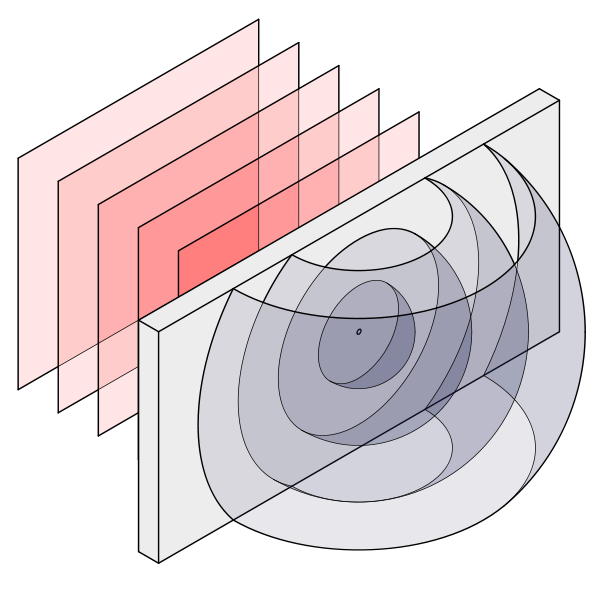
\includegraphics[width=150pt]{img/600px-Diffraction_through_Pinhole.png}
	\caption{A visualization of a wavefront diffracting through a pinhole much smaller than it's wavelength.}\cite{Diffraction}\label{fig:Diff}
\end{figure}
\subsection{Quantum Diffraction}
One of the fundamental concepts in quantum mechanics is that of wave-particle duality. This concept first originated with Einstein's idea that like, an electromagnetic wave, could also be propagated by discrete quantum particles, photons. From this de Broglie theorised the converse, if light has properties of both a wave and a particle, then all particles have properties of waves. The de Broglie wavelength of a particle was derived from rearranging the formulae for the Planck-Einstein relation, \[E=hf\] and momentum, \[p=\frac{E}{c}=\frac{h}{\lambda}\] where $f$ and $\lambda$ represent the frequency and wavelength, $c$ the speed of light, $h$ Planck's constant, into \[\lambda=\frac{h}{p}\] which relates momentum to the wavelength through Planck's constant. This relation holds true for particles, and this was experimentally proven using electrons. The Davisson-Germer experiment in 1927 involved firing electrons at a nickel target and measuring the intensity at the target. The intensity varied as the predicted diffraction pattern suggested, thus confirming de Broglie's hypothesis. Just as light diffracts when it interacts with physical objects, so can quantum particles.
A crystal lattice structure exhibits characteristic diffraction patterns when it interacts with waves, and de Broglie's ideas allow one to extend this idea to quantum particles as well. Huygen's principle means that each atom that interacts with a particle, becomes the source of it's own wave and this effect compounding with a fixed wavelength leads to diffraction patterns that can be used to infer details of the crystal lattice structure. The diffraction peaks of these patterns occur at certain angles relative to the planes in the crystal lattice and this relationship expresses itself as Bragg's Law: \[n\lambda=2d\sin{\theta}\]. In the case of crystal diffractometry, $d$ represents the spacing between lattice planes.\cite{Handout}\cite{Diffraction_Xray}
\subsection{Residual Stress}
When a material experiences a loading and subsequent unloading, there are some stresses left in the material. These stresses are known as residual stresses. Residual stresses are commonly left behind after various manufacturing techniques, sometimes they are a desired result, and sometimes they are a detrimental by-product. They can improve the strength and performance of materials, or weaken a material leading to undesired failure. A very common example of residual stresses being utilized to improve the performance of a material is tempered or toughened glass. 
Tempered glass is annealed glass (all residual stresses are relaxed prior to the tempering process) which undergoes either a chemical or thermal toughening procedure \cite{ToughGlass}. The thermal toughening procedure involves taking the annealed glass and heating it well above its transition temperature, approximately \SI{564}{\celsius}, before rapidly quenching. The glass is not completely cooled as the desired result is a solidified outer layer and an inner volume that is still above the transition temperature. Once the glass has fully cooled, the outer layers which experienced the quench are under a great deal of residual compressive stress and the inner volume, which was allowed to slowly cool, experiences a residual tensile stress. These residual stresses greatly improve the strength of the glass by allowing the outer surfaces to experience a much higher tensile load before failure.
\begin{figure}
	\centering
	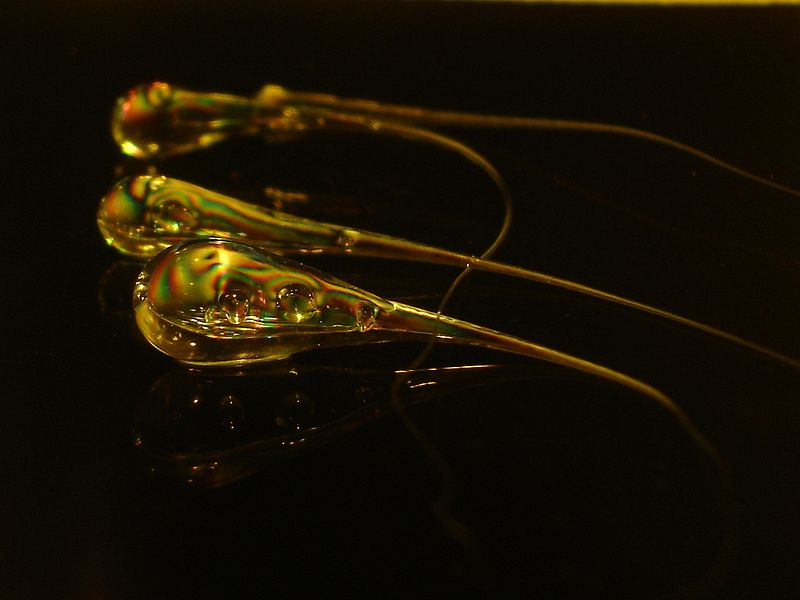
\includegraphics[width=250pt]{img/prince_rupert.jpg}
	\caption{Prince Rupert's drops are an extreme example of residual stresses in toughened glass}\cite{RupertDrop} \label{fig:RupertDrop}
\end{figure}
\subsection{Strain Measurement}
A strain diffractometer is a device that uses the principles of quantum mechanics and diffraction to provide insight into the behaviour of of material at the nano-scale. A material behaving elastically under an applied stress will have a corresponding strain in accordance with Hooke's Law. This strain manifests itself physically as an elongation but on the nano-scale it can be measured as a change in the atomic spacing of the material. This change in atomic spacing can be observed by comparing the positions of a diffraction peak, caused by the lattice structure in the material, before and after a stress is applied. This measurement technique is both non-destructive and non-contact, making it ideal for use in many engineering situations.
The output of the strain diffractometer will be two angles, those of the diffraction peak before, and while, the strain is applied. These angles can be converted into spacings using Bragg's Law, and further converted into strain ($\epsilon$) using the following formula where $d$ is the control spacing and $d'$ is the strained spacing.
\[
\epsilon = \frac{d'-d}{d}
\]
The region of material that is tested is known as the "Gauge Volume", and the measured strain represents the average value over this region. The gauge volume is formed at the intersection of the incoming beam and the diffracted beam. The direction that the strain is measured in is also the direction that bisects the two beams, thus is is important to take two (or three) perpendicular measurements in order to get a complete strain state.
It is important to not that this measurement technique will not measure any plastic strain in the sample. Elastic strain is caused by the change in lattice spacings due to applied stress, whereas plastic strain is the result of the movement of defects and displacements in the lattice of the material. Plastic strain does not affect the lattice spacing, only the location of atoms in the lattice.
\section{Experimental Details}
\subsection{Preparation of Samples}
The samples to undergo residual stress testing were cut from sheets of aluminium from a supplier based in Sydney. The stress was applied using a four point bending device and displacement was measured with a steel ruler. The four point bending device applied a pure bending moment load on the central \SI{100}{\milli\meter} region of the sample. The material outside this region was removed and discarded. The remaining material was analysed for residual stresses in the strain diffractometer. The four point 
\subsection{Testing of Mechanical Properties}
In order to determine the residual stress in a material by the neutron diffraction method, it is critical to know some of the important mechanical properties of the material. Namely: the Young's Modulus ($E$), and Poisson's Ratio ($\nu$). The Young's Modulus (or Modulus of Elasticity) is the relationship between stress ($\sigma$) and strain ($\epsilon$) in accordance with Hooke's Law.
$$\sigma = E\epsilon$$
Poisson's Ratio is used for stress and strain in three dimensions:

The mechanical properties of the materials were determined by the use of the University's tensile testing facilities on small samples of each material. The samples used were small 'dog-bone' coupons, cut from the original stock plates of aluminium. A schematic of these 'dog-bones' is shown below.

These coupons were put through a standard tensile test, involving the application of an increasing tensile load until failure while simultaneously recording measurements with a load cell and a strain gauge. Once the sample had passed passed it's yield stress and begun plastic deformation the strain gauge was removed the and load was increased to the point of failure. The final load ($F_F$), and ultimate strain ($\sigma_U$) are recorded in Table \ref{tab:a}.
\begin{table}[h]
	\centering
	\caption{Final load and ultimate strain measured for the tensile test coupons}\label{tab:a}
	\begin{tabular}[c]{c | c c}
	Sample & $F_F$ (\si{\mega\pascal}) & $\sigma_U$ \\ \hline\
	6061-T6 & 18.1 & 0.2 \\
	7075-T6 & 34.7 & 0.18 \\
	\end{tabular}
\end{table}
\subsection{Strain Measurement}
The strain diffractometry measurements were carried out at the KOWARI diffractometer at Sydney's Bragg Institute. A neutron wavelength of \SI{1.73}{\angstrom} was used to obtain \SI{90}{\degree} measurement geometry and a gauge volume of \SI{2x2x20}{\milli\meter} was used. Reference spacings ($d_0$) were obtained from an un-deformed sample of each material. \cite{Handout}
\begin{table}[h]
	\centering
	\caption{Reference ($d_0$) spacings}\label{tab:reference}
	\begin{tabular}[c]{c c}
	Sample & $d_0$ (\si{\angstrom}) \\ \hline \
	6061-T6 & $1.2181161 \pm 8\times10^{-6}$\\
	7075-T6 & $1.2188861 \pm 5\times10^{-6}$\\
	\end{tabular}
\end{table}
\subsection{Data Processing}
\subsubsection{Software}
All data was processed using Python3, as part of the Anaconda Data Science distribution \cite{Anaconda}. The data was taken in as a Numpy array, which is a numerical array computing library included in the Anaconda distribution, before being processed. The plots were created in Matplotlib, a plotting library that mirrors MATLAB's plotting functionality. Uncertainties were handled by the python Uncertainties library \cite{Uncertainties}. All the libraries used are open source, and the data processing code is included in the appendices.
\subsubsection{Determination of Elastic Properties}
Once the raw data had been gathered from the experiments it needed to be processed and used in calculations to determine the residual stress.
The first data-set to be processed was the stress/strain data as that would allow for the determination of the elastic properties of the two metals, allowing further calculations. The data, which consisted of two columns, gauge length and applied force, was loaded from text files to a Numpy array, then sorted by displacement values before being transformed into stress and strain values.
In order to find an elastic modulus ($E$) from this sorted data, a linear regression fit was carried out on the first 20\% of the data. This 20\% was chosen as it contained a linear region of the elastic behaviour of the metal, while being minimally affected by the non-linearities caused by plastic deformation. The results of this fit are recorded in Table \ref{tab:LinReg} and Figure \ref{fig:StressStrain} show plots of the stress/strain curve and the calculated elastic modulus.
\begin{table}[h!]
	\centering
	\caption{Linear Regression results for the stress/strain datasets}\label{tab:LinReg}
	\begin{tabular}[c]{c | c c c c}
	Sample & $E$ (\si{\giga\pascal}) & R value\\ \hline\
	6061-T6 & 71.73 & 0.9995 \\
	7075-T6 & 71.69 & 0.9997 \\
	\end{tabular}
\end{table}
\begin{figure}
	\centering
	\caption{Stress/Strain curves for 6061-T6 and 7075-T6 Aluminium samples}\label{fig:StressStrain}
	\scalebox{0.75}{%% Creator: Matplotlib, PGF backend
%%
%% To include the figure in your LaTeX document, write
%%   \input{<filename>.pgf}
%%
%% Make sure the required packages are loaded in your preamble
%%   \usepackage{pgf}
%%
%% Figures using additional raster images can only be included by \input if
%% they are in the same directory as the main LaTeX file. For loading figures
%% from other directories you can use the `import` package
%%   \usepackage{import}
%% and then include the figures with
%%   \import{<path to file>}{<filename>.pgf}
%%
%% Matplotlib used the following preamble
%%   \usepackage{siunitx}
%%   \usepackage{fontspec}
%%   \setmainfont{Times New Roman}
%%   \setsansfont{Lucida Grande}
%%   \setmonofont{Andale Mono}
%%
\begingroup%
\makeatletter%
\begin{pgfpicture}%
\pgfpathrectangle{\pgfpointorigin}{\pgfqpoint{6.400000in}{4.800000in}}%
\pgfusepath{use as bounding box, clip}%
\begin{pgfscope}%
\pgfsetbuttcap%
\pgfsetmiterjoin%
\definecolor{currentfill}{rgb}{1.000000,1.000000,1.000000}%
\pgfsetfillcolor{currentfill}%
\pgfsetlinewidth{0.000000pt}%
\definecolor{currentstroke}{rgb}{1.000000,1.000000,1.000000}%
\pgfsetstrokecolor{currentstroke}%
\pgfsetdash{}{0pt}%
\pgfpathmoveto{\pgfqpoint{0.000000in}{0.000000in}}%
\pgfpathlineto{\pgfqpoint{6.400000in}{0.000000in}}%
\pgfpathlineto{\pgfqpoint{6.400000in}{4.800000in}}%
\pgfpathlineto{\pgfqpoint{0.000000in}{4.800000in}}%
\pgfpathclose%
\pgfusepath{fill}%
\end{pgfscope}%
\begin{pgfscope}%
\pgfsetbuttcap%
\pgfsetmiterjoin%
\definecolor{currentfill}{rgb}{1.000000,1.000000,1.000000}%
\pgfsetfillcolor{currentfill}%
\pgfsetlinewidth{0.000000pt}%
\definecolor{currentstroke}{rgb}{0.000000,0.000000,0.000000}%
\pgfsetstrokecolor{currentstroke}%
\pgfsetstrokeopacity{0.000000}%
\pgfsetdash{}{0pt}%
\pgfpathmoveto{\pgfqpoint{0.800000in}{0.528000in}}%
\pgfpathlineto{\pgfqpoint{5.760000in}{0.528000in}}%
\pgfpathlineto{\pgfqpoint{5.760000in}{4.224000in}}%
\pgfpathlineto{\pgfqpoint{0.800000in}{4.224000in}}%
\pgfpathclose%
\pgfusepath{fill}%
\end{pgfscope}%
\begin{pgfscope}%
\pgfsetbuttcap%
\pgfsetroundjoin%
\definecolor{currentfill}{rgb}{0.000000,0.000000,0.000000}%
\pgfsetfillcolor{currentfill}%
\pgfsetlinewidth{0.803000pt}%
\definecolor{currentstroke}{rgb}{0.000000,0.000000,0.000000}%
\pgfsetstrokecolor{currentstroke}%
\pgfsetdash{}{0pt}%
\pgfsys@defobject{currentmarker}{\pgfqpoint{0.000000in}{-0.048611in}}{\pgfqpoint{0.000000in}{0.000000in}}{%
\pgfpathmoveto{\pgfqpoint{0.000000in}{0.000000in}}%
\pgfpathlineto{\pgfqpoint{0.000000in}{-0.048611in}}%
\pgfusepath{stroke,fill}%
}%
\begin{pgfscope}%
\pgfsys@transformshift{1.025455in}{0.528000in}%
\pgfsys@useobject{currentmarker}{}%
\end{pgfscope}%
\end{pgfscope}%
\begin{pgfscope}%
\pgftext[x=1.025455in,y=0.430778in,,top]{\sffamily\fontsize{10.000000}{12.000000}\selectfont 0.00}%
\end{pgfscope}%
\begin{pgfscope}%
\pgfsetbuttcap%
\pgfsetroundjoin%
\definecolor{currentfill}{rgb}{0.000000,0.000000,0.000000}%
\pgfsetfillcolor{currentfill}%
\pgfsetlinewidth{0.803000pt}%
\definecolor{currentstroke}{rgb}{0.000000,0.000000,0.000000}%
\pgfsetstrokecolor{currentstroke}%
\pgfsetdash{}{0pt}%
\pgfsys@defobject{currentmarker}{\pgfqpoint{0.000000in}{-0.048611in}}{\pgfqpoint{0.000000in}{0.000000in}}{%
\pgfpathmoveto{\pgfqpoint{0.000000in}{0.000000in}}%
\pgfpathlineto{\pgfqpoint{0.000000in}{-0.048611in}}%
\pgfusepath{stroke,fill}%
}%
\begin{pgfscope}%
\pgfsys@transformshift{1.959081in}{0.528000in}%
\pgfsys@useobject{currentmarker}{}%
\end{pgfscope}%
\end{pgfscope}%
\begin{pgfscope}%
\pgftext[x=1.959081in,y=0.430778in,,top]{\sffamily\fontsize{10.000000}{12.000000}\selectfont 0.01}%
\end{pgfscope}%
\begin{pgfscope}%
\pgfsetbuttcap%
\pgfsetroundjoin%
\definecolor{currentfill}{rgb}{0.000000,0.000000,0.000000}%
\pgfsetfillcolor{currentfill}%
\pgfsetlinewidth{0.803000pt}%
\definecolor{currentstroke}{rgb}{0.000000,0.000000,0.000000}%
\pgfsetstrokecolor{currentstroke}%
\pgfsetdash{}{0pt}%
\pgfsys@defobject{currentmarker}{\pgfqpoint{0.000000in}{-0.048611in}}{\pgfqpoint{0.000000in}{0.000000in}}{%
\pgfpathmoveto{\pgfqpoint{0.000000in}{0.000000in}}%
\pgfpathlineto{\pgfqpoint{0.000000in}{-0.048611in}}%
\pgfusepath{stroke,fill}%
}%
\begin{pgfscope}%
\pgfsys@transformshift{2.892708in}{0.528000in}%
\pgfsys@useobject{currentmarker}{}%
\end{pgfscope}%
\end{pgfscope}%
\begin{pgfscope}%
\pgftext[x=2.892708in,y=0.430778in,,top]{\sffamily\fontsize{10.000000}{12.000000}\selectfont 0.02}%
\end{pgfscope}%
\begin{pgfscope}%
\pgfsetbuttcap%
\pgfsetroundjoin%
\definecolor{currentfill}{rgb}{0.000000,0.000000,0.000000}%
\pgfsetfillcolor{currentfill}%
\pgfsetlinewidth{0.803000pt}%
\definecolor{currentstroke}{rgb}{0.000000,0.000000,0.000000}%
\pgfsetstrokecolor{currentstroke}%
\pgfsetdash{}{0pt}%
\pgfsys@defobject{currentmarker}{\pgfqpoint{0.000000in}{-0.048611in}}{\pgfqpoint{0.000000in}{0.000000in}}{%
\pgfpathmoveto{\pgfqpoint{0.000000in}{0.000000in}}%
\pgfpathlineto{\pgfqpoint{0.000000in}{-0.048611in}}%
\pgfusepath{stroke,fill}%
}%
\begin{pgfscope}%
\pgfsys@transformshift{3.826335in}{0.528000in}%
\pgfsys@useobject{currentmarker}{}%
\end{pgfscope}%
\end{pgfscope}%
\begin{pgfscope}%
\pgftext[x=3.826335in,y=0.430778in,,top]{\sffamily\fontsize{10.000000}{12.000000}\selectfont 0.03}%
\end{pgfscope}%
\begin{pgfscope}%
\pgfsetbuttcap%
\pgfsetroundjoin%
\definecolor{currentfill}{rgb}{0.000000,0.000000,0.000000}%
\pgfsetfillcolor{currentfill}%
\pgfsetlinewidth{0.803000pt}%
\definecolor{currentstroke}{rgb}{0.000000,0.000000,0.000000}%
\pgfsetstrokecolor{currentstroke}%
\pgfsetdash{}{0pt}%
\pgfsys@defobject{currentmarker}{\pgfqpoint{0.000000in}{-0.048611in}}{\pgfqpoint{0.000000in}{0.000000in}}{%
\pgfpathmoveto{\pgfqpoint{0.000000in}{0.000000in}}%
\pgfpathlineto{\pgfqpoint{0.000000in}{-0.048611in}}%
\pgfusepath{stroke,fill}%
}%
\begin{pgfscope}%
\pgfsys@transformshift{4.759961in}{0.528000in}%
\pgfsys@useobject{currentmarker}{}%
\end{pgfscope}%
\end{pgfscope}%
\begin{pgfscope}%
\pgftext[x=4.759961in,y=0.430778in,,top]{\sffamily\fontsize{10.000000}{12.000000}\selectfont 0.04}%
\end{pgfscope}%
\begin{pgfscope}%
\pgfsetbuttcap%
\pgfsetroundjoin%
\definecolor{currentfill}{rgb}{0.000000,0.000000,0.000000}%
\pgfsetfillcolor{currentfill}%
\pgfsetlinewidth{0.803000pt}%
\definecolor{currentstroke}{rgb}{0.000000,0.000000,0.000000}%
\pgfsetstrokecolor{currentstroke}%
\pgfsetdash{}{0pt}%
\pgfsys@defobject{currentmarker}{\pgfqpoint{0.000000in}{-0.048611in}}{\pgfqpoint{0.000000in}{0.000000in}}{%
\pgfpathmoveto{\pgfqpoint{0.000000in}{0.000000in}}%
\pgfpathlineto{\pgfqpoint{0.000000in}{-0.048611in}}%
\pgfusepath{stroke,fill}%
}%
\begin{pgfscope}%
\pgfsys@transformshift{5.693588in}{0.528000in}%
\pgfsys@useobject{currentmarker}{}%
\end{pgfscope}%
\end{pgfscope}%
\begin{pgfscope}%
\pgftext[x=5.693588in,y=0.430778in,,top]{\sffamily\fontsize{10.000000}{12.000000}\selectfont 0.05}%
\end{pgfscope}%
\begin{pgfscope}%
\pgftext[x=3.280000in,y=0.241352in,,top]{\sffamily\fontsize{10.000000}{12.000000}\selectfont \(\displaystyle \epsilon\)}%
\end{pgfscope}%
\begin{pgfscope}%
\pgfsetbuttcap%
\pgfsetroundjoin%
\definecolor{currentfill}{rgb}{0.000000,0.000000,0.000000}%
\pgfsetfillcolor{currentfill}%
\pgfsetlinewidth{0.803000pt}%
\definecolor{currentstroke}{rgb}{0.000000,0.000000,0.000000}%
\pgfsetstrokecolor{currentstroke}%
\pgfsetdash{}{0pt}%
\pgfsys@defobject{currentmarker}{\pgfqpoint{-0.048611in}{0.000000in}}{\pgfqpoint{0.000000in}{0.000000in}}{%
\pgfpathmoveto{\pgfqpoint{0.000000in}{0.000000in}}%
\pgfpathlineto{\pgfqpoint{-0.048611in}{0.000000in}}%
\pgfusepath{stroke,fill}%
}%
\begin{pgfscope}%
\pgfsys@transformshift{0.800000in}{0.670776in}%
\pgfsys@useobject{currentmarker}{}%
\end{pgfscope}%
\end{pgfscope}%
\begin{pgfscope}%
\pgftext[x=0.483187in,y=0.617235in,left,base]{\sffamily\fontsize{10.000000}{12.000000}\selectfont 0.0}%
\end{pgfscope}%
\begin{pgfscope}%
\pgfsetbuttcap%
\pgfsetroundjoin%
\definecolor{currentfill}{rgb}{0.000000,0.000000,0.000000}%
\pgfsetfillcolor{currentfill}%
\pgfsetlinewidth{0.803000pt}%
\definecolor{currentstroke}{rgb}{0.000000,0.000000,0.000000}%
\pgfsetstrokecolor{currentstroke}%
\pgfsetdash{}{0pt}%
\pgfsys@defobject{currentmarker}{\pgfqpoint{-0.048611in}{0.000000in}}{\pgfqpoint{0.000000in}{0.000000in}}{%
\pgfpathmoveto{\pgfqpoint{0.000000in}{0.000000in}}%
\pgfpathlineto{\pgfqpoint{-0.048611in}{0.000000in}}%
\pgfusepath{stroke,fill}%
}%
\begin{pgfscope}%
\pgfsys@transformshift{0.800000in}{1.229066in}%
\pgfsys@useobject{currentmarker}{}%
\end{pgfscope}%
\end{pgfscope}%
\begin{pgfscope}%
\pgftext[x=0.483187in,y=1.175524in,left,base]{\sffamily\fontsize{10.000000}{12.000000}\selectfont 0.5}%
\end{pgfscope}%
\begin{pgfscope}%
\pgfsetbuttcap%
\pgfsetroundjoin%
\definecolor{currentfill}{rgb}{0.000000,0.000000,0.000000}%
\pgfsetfillcolor{currentfill}%
\pgfsetlinewidth{0.803000pt}%
\definecolor{currentstroke}{rgb}{0.000000,0.000000,0.000000}%
\pgfsetstrokecolor{currentstroke}%
\pgfsetdash{}{0pt}%
\pgfsys@defobject{currentmarker}{\pgfqpoint{-0.048611in}{0.000000in}}{\pgfqpoint{0.000000in}{0.000000in}}{%
\pgfpathmoveto{\pgfqpoint{0.000000in}{0.000000in}}%
\pgfpathlineto{\pgfqpoint{-0.048611in}{0.000000in}}%
\pgfusepath{stroke,fill}%
}%
\begin{pgfscope}%
\pgfsys@transformshift{0.800000in}{1.787355in}%
\pgfsys@useobject{currentmarker}{}%
\end{pgfscope}%
\end{pgfscope}%
\begin{pgfscope}%
\pgftext[x=0.483187in,y=1.733814in,left,base]{\sffamily\fontsize{10.000000}{12.000000}\selectfont 1.0}%
\end{pgfscope}%
\begin{pgfscope}%
\pgfsetbuttcap%
\pgfsetroundjoin%
\definecolor{currentfill}{rgb}{0.000000,0.000000,0.000000}%
\pgfsetfillcolor{currentfill}%
\pgfsetlinewidth{0.803000pt}%
\definecolor{currentstroke}{rgb}{0.000000,0.000000,0.000000}%
\pgfsetstrokecolor{currentstroke}%
\pgfsetdash{}{0pt}%
\pgfsys@defobject{currentmarker}{\pgfqpoint{-0.048611in}{0.000000in}}{\pgfqpoint{0.000000in}{0.000000in}}{%
\pgfpathmoveto{\pgfqpoint{0.000000in}{0.000000in}}%
\pgfpathlineto{\pgfqpoint{-0.048611in}{0.000000in}}%
\pgfusepath{stroke,fill}%
}%
\begin{pgfscope}%
\pgfsys@transformshift{0.800000in}{2.345645in}%
\pgfsys@useobject{currentmarker}{}%
\end{pgfscope}%
\end{pgfscope}%
\begin{pgfscope}%
\pgftext[x=0.483187in,y=2.292103in,left,base]{\sffamily\fontsize{10.000000}{12.000000}\selectfont 1.5}%
\end{pgfscope}%
\begin{pgfscope}%
\pgfsetbuttcap%
\pgfsetroundjoin%
\definecolor{currentfill}{rgb}{0.000000,0.000000,0.000000}%
\pgfsetfillcolor{currentfill}%
\pgfsetlinewidth{0.803000pt}%
\definecolor{currentstroke}{rgb}{0.000000,0.000000,0.000000}%
\pgfsetstrokecolor{currentstroke}%
\pgfsetdash{}{0pt}%
\pgfsys@defobject{currentmarker}{\pgfqpoint{-0.048611in}{0.000000in}}{\pgfqpoint{0.000000in}{0.000000in}}{%
\pgfpathmoveto{\pgfqpoint{0.000000in}{0.000000in}}%
\pgfpathlineto{\pgfqpoint{-0.048611in}{0.000000in}}%
\pgfusepath{stroke,fill}%
}%
\begin{pgfscope}%
\pgfsys@transformshift{0.800000in}{2.903934in}%
\pgfsys@useobject{currentmarker}{}%
\end{pgfscope}%
\end{pgfscope}%
\begin{pgfscope}%
\pgftext[x=0.483187in,y=2.850393in,left,base]{\sffamily\fontsize{10.000000}{12.000000}\selectfont 2.0}%
\end{pgfscope}%
\begin{pgfscope}%
\pgfsetbuttcap%
\pgfsetroundjoin%
\definecolor{currentfill}{rgb}{0.000000,0.000000,0.000000}%
\pgfsetfillcolor{currentfill}%
\pgfsetlinewidth{0.803000pt}%
\definecolor{currentstroke}{rgb}{0.000000,0.000000,0.000000}%
\pgfsetstrokecolor{currentstroke}%
\pgfsetdash{}{0pt}%
\pgfsys@defobject{currentmarker}{\pgfqpoint{-0.048611in}{0.000000in}}{\pgfqpoint{0.000000in}{0.000000in}}{%
\pgfpathmoveto{\pgfqpoint{0.000000in}{0.000000in}}%
\pgfpathlineto{\pgfqpoint{-0.048611in}{0.000000in}}%
\pgfusepath{stroke,fill}%
}%
\begin{pgfscope}%
\pgfsys@transformshift{0.800000in}{3.462224in}%
\pgfsys@useobject{currentmarker}{}%
\end{pgfscope}%
\end{pgfscope}%
\begin{pgfscope}%
\pgftext[x=0.483187in,y=3.408682in,left,base]{\sffamily\fontsize{10.000000}{12.000000}\selectfont 2.5}%
\end{pgfscope}%
\begin{pgfscope}%
\pgfsetbuttcap%
\pgfsetroundjoin%
\definecolor{currentfill}{rgb}{0.000000,0.000000,0.000000}%
\pgfsetfillcolor{currentfill}%
\pgfsetlinewidth{0.803000pt}%
\definecolor{currentstroke}{rgb}{0.000000,0.000000,0.000000}%
\pgfsetstrokecolor{currentstroke}%
\pgfsetdash{}{0pt}%
\pgfsys@defobject{currentmarker}{\pgfqpoint{-0.048611in}{0.000000in}}{\pgfqpoint{0.000000in}{0.000000in}}{%
\pgfpathmoveto{\pgfqpoint{0.000000in}{0.000000in}}%
\pgfpathlineto{\pgfqpoint{-0.048611in}{0.000000in}}%
\pgfusepath{stroke,fill}%
}%
\begin{pgfscope}%
\pgfsys@transformshift{0.800000in}{4.020513in}%
\pgfsys@useobject{currentmarker}{}%
\end{pgfscope}%
\end{pgfscope}%
\begin{pgfscope}%
\pgftext[x=0.483187in,y=3.966972in,left,base]{\sffamily\fontsize{10.000000}{12.000000}\selectfont 3.0}%
\end{pgfscope}%
\begin{pgfscope}%
\pgftext[x=0.427631in,y=2.376000in,,bottom,rotate=90.000000]{\sffamily\fontsize{10.000000}{12.000000}\selectfont \(\displaystyle \sigma (\si{\pascal})\)}%
\end{pgfscope}%
\begin{pgfscope}%
\pgftext[x=0.800000in,y=4.265667in,left,base]{\sffamily\fontsize{10.000000}{12.000000}\selectfont 1e8}%
\end{pgfscope}%
\begin{pgfscope}%
\pgfpathrectangle{\pgfqpoint{0.800000in}{0.528000in}}{\pgfqpoint{4.960000in}{3.696000in}} %
\pgfusepath{clip}%
\pgfsetrectcap%
\pgfsetroundjoin%
\pgfsetlinewidth{1.505625pt}%
\definecolor{currentstroke}{rgb}{0.121569,0.466667,0.705882}%
\pgfsetstrokecolor{currentstroke}%
\pgfsetdash{}{0pt}%
\pgfpathmoveto{\pgfqpoint{1.025455in}{0.696000in}}%
\pgfpathlineto{\pgfqpoint{1.038995in}{0.796947in}}%
\pgfpathlineto{\pgfqpoint{1.048023in}{0.831734in}}%
\pgfpathlineto{\pgfqpoint{1.057050in}{0.893241in}}%
\pgfpathlineto{\pgfqpoint{1.079618in}{1.093082in}}%
\pgfpathlineto{\pgfqpoint{1.115727in}{1.400687in}}%
\pgfpathlineto{\pgfqpoint{1.129267in}{1.525789in}}%
\pgfpathlineto{\pgfqpoint{1.169890in}{1.874179in}}%
\pgfpathlineto{\pgfqpoint{1.368488in}{3.665164in}}%
\pgfpathlineto{\pgfqpoint{1.382029in}{3.756865in}}%
\pgfpathlineto{\pgfqpoint{1.386543in}{3.784576in}}%
\pgfpathlineto{\pgfqpoint{1.395570in}{3.823853in}}%
\pgfpathlineto{\pgfqpoint{1.404597in}{3.853881in}}%
\pgfpathlineto{\pgfqpoint{1.409111in}{3.861280in}}%
\pgfpathlineto{\pgfqpoint{1.418138in}{3.881065in}}%
\pgfpathlineto{\pgfqpoint{1.436193in}{3.904456in}}%
\pgfpathlineto{\pgfqpoint{1.440706in}{3.907026in}}%
\pgfpathlineto{\pgfqpoint{1.454247in}{3.919122in}}%
\pgfpathlineto{\pgfqpoint{1.467788in}{3.924733in}}%
\pgfpathlineto{\pgfqpoint{1.476815in}{3.931066in}}%
\pgfpathlineto{\pgfqpoint{1.481329in}{3.931794in}}%
\pgfpathlineto{\pgfqpoint{1.499383in}{3.939233in}}%
\pgfpathlineto{\pgfqpoint{1.503897in}{3.940286in}}%
\pgfpathlineto{\pgfqpoint{1.508410in}{3.943207in}}%
\pgfpathlineto{\pgfqpoint{1.517437in}{3.946106in}}%
\pgfpathlineto{\pgfqpoint{1.521951in}{3.944865in}}%
\pgfpathlineto{\pgfqpoint{1.526465in}{3.947914in}}%
\pgfpathlineto{\pgfqpoint{1.540005in}{3.950176in}}%
\pgfpathlineto{\pgfqpoint{1.567087in}{3.956056in}}%
\pgfpathlineto{\pgfqpoint{1.571601in}{3.954809in}}%
\pgfpathlineto{\pgfqpoint{1.585142in}{3.957701in}}%
\pgfpathlineto{\pgfqpoint{1.594169in}{3.958639in}}%
\pgfpathlineto{\pgfqpoint{1.598682in}{3.962584in}}%
\pgfpathlineto{\pgfqpoint{1.603196in}{3.962349in}}%
\pgfpathlineto{\pgfqpoint{1.607710in}{3.960254in}}%
\pgfpathlineto{\pgfqpoint{1.612223in}{3.960269in}}%
\pgfpathlineto{\pgfqpoint{1.621250in}{3.963719in}}%
\pgfpathlineto{\pgfqpoint{1.625764in}{3.964964in}}%
\pgfpathlineto{\pgfqpoint{1.630278in}{3.964269in}}%
\pgfpathlineto{\pgfqpoint{1.634791in}{3.966626in}}%
\pgfpathlineto{\pgfqpoint{1.648332in}{3.965429in}}%
\pgfpathlineto{\pgfqpoint{1.661873in}{3.967705in}}%
\pgfpathlineto{\pgfqpoint{1.666386in}{3.967895in}}%
\pgfpathlineto{\pgfqpoint{1.675414in}{3.969723in}}%
\pgfpathlineto{\pgfqpoint{1.684441in}{3.970525in}}%
\pgfpathlineto{\pgfqpoint{1.688954in}{3.969650in}}%
\pgfpathlineto{\pgfqpoint{1.693468in}{3.970403in}}%
\pgfpathlineto{\pgfqpoint{1.697982in}{3.969001in}}%
\pgfpathlineto{\pgfqpoint{1.716036in}{3.971874in}}%
\pgfpathlineto{\pgfqpoint{1.729577in}{3.972174in}}%
\pgfpathlineto{\pgfqpoint{1.738604in}{3.974788in}}%
\pgfpathlineto{\pgfqpoint{1.743118in}{3.974835in}}%
\pgfpathlineto{\pgfqpoint{1.747631in}{3.973525in}}%
\pgfpathlineto{\pgfqpoint{1.761172in}{3.975034in}}%
\pgfpathlineto{\pgfqpoint{1.765686in}{3.973847in}}%
\pgfpathlineto{\pgfqpoint{1.770199in}{3.974706in}}%
\pgfpathlineto{\pgfqpoint{1.774713in}{3.974117in}}%
\pgfpathlineto{\pgfqpoint{1.779226in}{3.975183in}}%
\pgfpathlineto{\pgfqpoint{1.783740in}{3.974831in}}%
\pgfpathlineto{\pgfqpoint{1.788254in}{3.977088in}}%
\pgfpathlineto{\pgfqpoint{1.792767in}{3.976862in}}%
\pgfpathlineto{\pgfqpoint{1.797281in}{3.978484in}}%
\pgfpathlineto{\pgfqpoint{1.824363in}{3.975366in}}%
\pgfpathlineto{\pgfqpoint{1.833390in}{3.978274in}}%
\pgfpathlineto{\pgfqpoint{1.842417in}{3.977308in}}%
\pgfpathlineto{\pgfqpoint{1.846931in}{3.977614in}}%
\pgfpathlineto{\pgfqpoint{1.851444in}{3.979809in}}%
\pgfpathlineto{\pgfqpoint{1.860471in}{3.980893in}}%
\pgfpathlineto{\pgfqpoint{1.878526in}{3.978950in}}%
\pgfpathlineto{\pgfqpoint{1.883039in}{3.980957in}}%
\pgfpathlineto{\pgfqpoint{1.892067in}{3.979586in}}%
\pgfpathlineto{\pgfqpoint{1.905607in}{3.981060in}}%
\pgfpathlineto{\pgfqpoint{1.914635in}{3.979096in}}%
\pgfpathlineto{\pgfqpoint{1.919148in}{3.979273in}}%
\pgfpathlineto{\pgfqpoint{1.923662in}{3.981040in}}%
\pgfpathlineto{\pgfqpoint{1.941716in}{3.982200in}}%
\pgfpathlineto{\pgfqpoint{1.946230in}{3.982231in}}%
\pgfpathlineto{\pgfqpoint{1.950743in}{3.980509in}}%
\pgfpathlineto{\pgfqpoint{1.955257in}{3.982924in}}%
\pgfpathlineto{\pgfqpoint{1.959771in}{3.982507in}}%
\pgfpathlineto{\pgfqpoint{1.964284in}{3.980601in}}%
\pgfpathlineto{\pgfqpoint{1.968798in}{3.982718in}}%
\pgfpathlineto{\pgfqpoint{2.004907in}{3.985554in}}%
\pgfpathlineto{\pgfqpoint{2.009420in}{3.983409in}}%
\pgfpathlineto{\pgfqpoint{2.013934in}{3.984149in}}%
\pgfpathlineto{\pgfqpoint{2.027475in}{3.982700in}}%
\pgfpathlineto{\pgfqpoint{2.036502in}{3.984109in}}%
\pgfpathlineto{\pgfqpoint{2.041016in}{3.984830in}}%
\pgfpathlineto{\pgfqpoint{2.045529in}{3.987211in}}%
\pgfpathlineto{\pgfqpoint{2.054556in}{3.985492in}}%
\pgfpathlineto{\pgfqpoint{2.068097in}{3.985800in}}%
\pgfpathlineto{\pgfqpoint{2.077124in}{3.984287in}}%
\pgfpathlineto{\pgfqpoint{2.086152in}{3.986115in}}%
\pgfpathlineto{\pgfqpoint{2.090665in}{3.985183in}}%
\pgfpathlineto{\pgfqpoint{2.104206in}{3.987316in}}%
\pgfpathlineto{\pgfqpoint{2.108720in}{3.985599in}}%
\pgfpathlineto{\pgfqpoint{2.117747in}{3.987153in}}%
\pgfpathlineto{\pgfqpoint{2.126774in}{3.985342in}}%
\pgfpathlineto{\pgfqpoint{2.140315in}{3.987783in}}%
\pgfpathlineto{\pgfqpoint{2.144828in}{3.988856in}}%
\pgfpathlineto{\pgfqpoint{2.158369in}{3.986499in}}%
\pgfpathlineto{\pgfqpoint{2.162883in}{3.987348in}}%
\pgfpathlineto{\pgfqpoint{2.176424in}{3.987150in}}%
\pgfpathlineto{\pgfqpoint{2.185451in}{3.989488in}}%
\pgfpathlineto{\pgfqpoint{2.194478in}{3.987781in}}%
\pgfpathlineto{\pgfqpoint{2.217046in}{3.989258in}}%
\pgfpathlineto{\pgfqpoint{2.226073in}{3.988498in}}%
\pgfpathlineto{\pgfqpoint{2.230587in}{3.988112in}}%
\pgfpathlineto{\pgfqpoint{2.235101in}{3.989512in}}%
\pgfpathlineto{\pgfqpoint{2.239614in}{3.988859in}}%
\pgfpathlineto{\pgfqpoint{2.244128in}{3.990830in}}%
\pgfpathlineto{\pgfqpoint{2.253155in}{3.990386in}}%
\pgfpathlineto{\pgfqpoint{2.257669in}{3.988061in}}%
\pgfpathlineto{\pgfqpoint{2.262182in}{3.988774in}}%
\pgfpathlineto{\pgfqpoint{2.266696in}{3.990720in}}%
\pgfpathlineto{\pgfqpoint{2.284750in}{3.989595in}}%
\pgfpathlineto{\pgfqpoint{2.298291in}{3.991412in}}%
\pgfpathlineto{\pgfqpoint{2.302805in}{3.989895in}}%
\pgfpathlineto{\pgfqpoint{2.307318in}{3.991797in}}%
\pgfpathlineto{\pgfqpoint{2.311832in}{3.990266in}}%
\pgfpathlineto{\pgfqpoint{2.316345in}{3.991743in}}%
\pgfpathlineto{\pgfqpoint{2.325373in}{3.991582in}}%
\pgfpathlineto{\pgfqpoint{2.338913in}{3.991256in}}%
\pgfpathlineto{\pgfqpoint{2.343427in}{3.989436in}}%
\pgfpathlineto{\pgfqpoint{2.347941in}{3.991204in}}%
\pgfpathlineto{\pgfqpoint{2.361481in}{3.990064in}}%
\pgfpathlineto{\pgfqpoint{2.365995in}{3.991422in}}%
\pgfpathlineto{\pgfqpoint{2.393077in}{3.990941in}}%
\pgfpathlineto{\pgfqpoint{2.397590in}{3.993131in}}%
\pgfpathlineto{\pgfqpoint{2.402104in}{3.993974in}}%
\pgfpathlineto{\pgfqpoint{2.406618in}{3.992956in}}%
\pgfpathlineto{\pgfqpoint{2.411131in}{3.993271in}}%
\pgfpathlineto{\pgfqpoint{2.415645in}{3.992466in}}%
\pgfpathlineto{\pgfqpoint{2.420158in}{3.993068in}}%
\pgfpathlineto{\pgfqpoint{2.424672in}{3.991983in}}%
\pgfpathlineto{\pgfqpoint{2.433699in}{3.994328in}}%
\pgfpathlineto{\pgfqpoint{2.456267in}{3.993846in}}%
\pgfpathlineto{\pgfqpoint{2.460781in}{3.995159in}}%
\pgfpathlineto{\pgfqpoint{2.469808in}{3.993602in}}%
\pgfpathlineto{\pgfqpoint{2.478835in}{3.992927in}}%
\pgfpathlineto{\pgfqpoint{2.483349in}{3.993219in}}%
\pgfpathlineto{\pgfqpoint{2.487862in}{3.995009in}}%
\pgfpathlineto{\pgfqpoint{2.496890in}{3.994832in}}%
\pgfpathlineto{\pgfqpoint{2.501403in}{3.996136in}}%
\pgfpathlineto{\pgfqpoint{2.505917in}{3.994154in}}%
\pgfpathlineto{\pgfqpoint{2.519458in}{3.994640in}}%
\pgfpathlineto{\pgfqpoint{2.528485in}{3.995747in}}%
\pgfpathlineto{\pgfqpoint{2.532998in}{3.994447in}}%
\pgfpathlineto{\pgfqpoint{2.537512in}{3.995185in}}%
\pgfpathlineto{\pgfqpoint{2.542026in}{3.994128in}}%
\pgfpathlineto{\pgfqpoint{2.551053in}{3.995011in}}%
\pgfpathlineto{\pgfqpoint{2.560080in}{3.993682in}}%
\pgfpathlineto{\pgfqpoint{2.564594in}{3.995809in}}%
\pgfpathlineto{\pgfqpoint{2.573621in}{3.995515in}}%
\pgfpathlineto{\pgfqpoint{2.582648in}{3.996722in}}%
\pgfpathlineto{\pgfqpoint{2.587162in}{3.995637in}}%
\pgfpathlineto{\pgfqpoint{2.591675in}{3.996319in}}%
\pgfpathlineto{\pgfqpoint{2.596189in}{3.994343in}}%
\pgfpathlineto{\pgfqpoint{2.605216in}{3.997275in}}%
\pgfpathlineto{\pgfqpoint{2.609730in}{3.995786in}}%
\pgfpathlineto{\pgfqpoint{2.627784in}{3.996607in}}%
\pgfpathlineto{\pgfqpoint{2.632298in}{3.994617in}}%
\pgfpathlineto{\pgfqpoint{2.636811in}{3.994623in}}%
\pgfpathlineto{\pgfqpoint{2.641325in}{3.997007in}}%
\pgfpathlineto{\pgfqpoint{2.645839in}{3.996613in}}%
\pgfpathlineto{\pgfqpoint{2.650352in}{3.998127in}}%
\pgfpathlineto{\pgfqpoint{2.659379in}{3.997490in}}%
\pgfpathlineto{\pgfqpoint{2.668407in}{3.997282in}}%
\pgfpathlineto{\pgfqpoint{2.677434in}{3.997540in}}%
\pgfpathlineto{\pgfqpoint{2.681947in}{3.996060in}}%
\pgfpathlineto{\pgfqpoint{2.686461in}{3.997497in}}%
\pgfpathlineto{\pgfqpoint{2.695488in}{3.996714in}}%
\pgfpathlineto{\pgfqpoint{2.700002in}{3.998686in}}%
\pgfpathlineto{\pgfqpoint{2.709029in}{4.000126in}}%
\pgfpathlineto{\pgfqpoint{2.718056in}{3.996219in}}%
\pgfpathlineto{\pgfqpoint{2.731597in}{3.997608in}}%
\pgfpathlineto{\pgfqpoint{2.763192in}{3.998707in}}%
\pgfpathlineto{\pgfqpoint{2.767706in}{4.000819in}}%
\pgfpathlineto{\pgfqpoint{2.781247in}{3.998986in}}%
\pgfpathlineto{\pgfqpoint{2.785760in}{3.999208in}}%
\pgfpathlineto{\pgfqpoint{2.790274in}{4.001125in}}%
\pgfpathlineto{\pgfqpoint{2.803815in}{3.998805in}}%
\pgfpathlineto{\pgfqpoint{2.808328in}{4.000766in}}%
\pgfpathlineto{\pgfqpoint{2.812842in}{3.999687in}}%
\pgfpathlineto{\pgfqpoint{2.817356in}{4.000648in}}%
\pgfpathlineto{\pgfqpoint{2.821869in}{4.000404in}}%
\pgfpathlineto{\pgfqpoint{2.826383in}{3.998945in}}%
\pgfpathlineto{\pgfqpoint{2.830896in}{3.999577in}}%
\pgfpathlineto{\pgfqpoint{2.835410in}{3.998862in}}%
\pgfpathlineto{\pgfqpoint{2.844437in}{4.000522in}}%
\pgfpathlineto{\pgfqpoint{2.848951in}{3.999597in}}%
\pgfpathlineto{\pgfqpoint{2.853464in}{4.000699in}}%
\pgfpathlineto{\pgfqpoint{2.857978in}{3.999785in}}%
\pgfpathlineto{\pgfqpoint{2.862492in}{4.001772in}}%
\pgfpathlineto{\pgfqpoint{2.876032in}{4.000265in}}%
\pgfpathlineto{\pgfqpoint{2.880546in}{4.002999in}}%
\pgfpathlineto{\pgfqpoint{2.885060in}{4.000813in}}%
\pgfpathlineto{\pgfqpoint{2.894087in}{3.999191in}}%
\pgfpathlineto{\pgfqpoint{2.898600in}{4.000498in}}%
\pgfpathlineto{\pgfqpoint{2.907628in}{3.998261in}}%
\pgfpathlineto{\pgfqpoint{2.939223in}{4.003844in}}%
\pgfpathlineto{\pgfqpoint{2.948250in}{4.002883in}}%
\pgfpathlineto{\pgfqpoint{2.952764in}{4.002395in}}%
\pgfpathlineto{\pgfqpoint{2.961791in}{4.003836in}}%
\pgfpathlineto{\pgfqpoint{2.970818in}{4.002441in}}%
\pgfpathlineto{\pgfqpoint{2.979845in}{4.003325in}}%
\pgfpathlineto{\pgfqpoint{2.984359in}{4.001719in}}%
\pgfpathlineto{\pgfqpoint{2.988873in}{4.003431in}}%
\pgfpathlineto{\pgfqpoint{2.993386in}{4.002882in}}%
\pgfpathlineto{\pgfqpoint{2.997900in}{4.004207in}}%
\pgfpathlineto{\pgfqpoint{3.002413in}{4.003870in}}%
\pgfpathlineto{\pgfqpoint{3.006927in}{4.005630in}}%
\pgfpathlineto{\pgfqpoint{3.011441in}{4.003914in}}%
\pgfpathlineto{\pgfqpoint{3.015954in}{4.004674in}}%
\pgfpathlineto{\pgfqpoint{3.024981in}{4.002425in}}%
\pgfpathlineto{\pgfqpoint{3.038522in}{4.004586in}}%
\pgfpathlineto{\pgfqpoint{3.047549in}{4.003917in}}%
\pgfpathlineto{\pgfqpoint{3.052063in}{4.005362in}}%
\pgfpathlineto{\pgfqpoint{3.056577in}{4.002763in}}%
\pgfpathlineto{\pgfqpoint{3.061090in}{4.004770in}}%
\pgfpathlineto{\pgfqpoint{3.070117in}{4.003756in}}%
\pgfpathlineto{\pgfqpoint{3.079145in}{4.004194in}}%
\pgfpathlineto{\pgfqpoint{3.169417in}{4.006015in}}%
\pgfpathlineto{\pgfqpoint{3.173930in}{4.005436in}}%
\pgfpathlineto{\pgfqpoint{3.182958in}{4.008196in}}%
\pgfpathlineto{\pgfqpoint{3.187471in}{4.006526in}}%
\pgfpathlineto{\pgfqpoint{3.196498in}{4.006207in}}%
\pgfpathlineto{\pgfqpoint{3.210039in}{4.004686in}}%
\pgfpathlineto{\pgfqpoint{3.214553in}{4.003918in}}%
\pgfpathlineto{\pgfqpoint{3.223580in}{4.007156in}}%
\pgfpathlineto{\pgfqpoint{3.232607in}{4.007568in}}%
\pgfpathlineto{\pgfqpoint{3.246148in}{4.006866in}}%
\pgfpathlineto{\pgfqpoint{3.250662in}{4.005248in}}%
\pgfpathlineto{\pgfqpoint{3.259689in}{4.006073in}}%
\pgfpathlineto{\pgfqpoint{3.264202in}{4.007862in}}%
\pgfpathlineto{\pgfqpoint{3.268716in}{4.007904in}}%
\pgfpathlineto{\pgfqpoint{3.273230in}{4.009203in}}%
\pgfpathlineto{\pgfqpoint{3.277743in}{4.009140in}}%
\pgfpathlineto{\pgfqpoint{3.282257in}{4.010326in}}%
\pgfpathlineto{\pgfqpoint{3.304825in}{4.008869in}}%
\pgfpathlineto{\pgfqpoint{3.309338in}{4.010050in}}%
\pgfpathlineto{\pgfqpoint{3.313852in}{4.009528in}}%
\pgfpathlineto{\pgfqpoint{3.318366in}{4.010368in}}%
\pgfpathlineto{\pgfqpoint{3.327393in}{4.008692in}}%
\pgfpathlineto{\pgfqpoint{3.331906in}{4.010415in}}%
\pgfpathlineto{\pgfqpoint{3.336420in}{4.009283in}}%
\pgfpathlineto{\pgfqpoint{3.340934in}{4.009672in}}%
\pgfpathlineto{\pgfqpoint{3.345447in}{4.007705in}}%
\pgfpathlineto{\pgfqpoint{3.368015in}{4.009404in}}%
\pgfpathlineto{\pgfqpoint{3.381556in}{4.008667in}}%
\pgfpathlineto{\pgfqpoint{3.386070in}{4.011388in}}%
\pgfpathlineto{\pgfqpoint{3.395097in}{4.011481in}}%
\pgfpathlineto{\pgfqpoint{3.404124in}{4.009981in}}%
\pgfpathlineto{\pgfqpoint{3.408638in}{4.007652in}}%
\pgfpathlineto{\pgfqpoint{3.413151in}{4.010356in}}%
\pgfpathlineto{\pgfqpoint{3.422179in}{4.009766in}}%
\pgfpathlineto{\pgfqpoint{3.431206in}{4.009239in}}%
\pgfpathlineto{\pgfqpoint{3.435719in}{4.011127in}}%
\pgfpathlineto{\pgfqpoint{3.440233in}{4.009575in}}%
\pgfpathlineto{\pgfqpoint{3.453774in}{4.013485in}}%
\pgfpathlineto{\pgfqpoint{3.458287in}{4.012324in}}%
\pgfpathlineto{\pgfqpoint{3.462801in}{4.014048in}}%
\pgfpathlineto{\pgfqpoint{3.471828in}{4.014348in}}%
\pgfpathlineto{\pgfqpoint{3.476342in}{4.012467in}}%
\pgfpathlineto{\pgfqpoint{3.489883in}{4.011872in}}%
\pgfpathlineto{\pgfqpoint{3.498910in}{4.011768in}}%
\pgfpathlineto{\pgfqpoint{3.503423in}{4.013945in}}%
\pgfpathlineto{\pgfqpoint{3.512451in}{4.013727in}}%
\pgfpathlineto{\pgfqpoint{3.521478in}{4.012481in}}%
\pgfpathlineto{\pgfqpoint{3.525991in}{4.013589in}}%
\pgfpathlineto{\pgfqpoint{3.535019in}{4.011957in}}%
\pgfpathlineto{\pgfqpoint{3.539532in}{4.010766in}}%
\pgfpathlineto{\pgfqpoint{3.544046in}{4.013536in}}%
\pgfpathlineto{\pgfqpoint{3.548559in}{4.013078in}}%
\pgfpathlineto{\pgfqpoint{3.553073in}{4.014333in}}%
\pgfpathlineto{\pgfqpoint{3.571127in}{4.013989in}}%
\pgfpathlineto{\pgfqpoint{3.575641in}{4.016086in}}%
\pgfpathlineto{\pgfqpoint{3.580155in}{4.014364in}}%
\pgfpathlineto{\pgfqpoint{3.602723in}{4.013496in}}%
\pgfpathlineto{\pgfqpoint{3.607236in}{4.014482in}}%
\pgfpathlineto{\pgfqpoint{3.611750in}{4.014250in}}%
\pgfpathlineto{\pgfqpoint{3.616264in}{4.015824in}}%
\pgfpathlineto{\pgfqpoint{3.629804in}{4.014514in}}%
\pgfpathlineto{\pgfqpoint{3.634318in}{4.015643in}}%
\pgfpathlineto{\pgfqpoint{3.661400in}{4.015802in}}%
\pgfpathlineto{\pgfqpoint{3.665913in}{4.016739in}}%
\pgfpathlineto{\pgfqpoint{3.674940in}{4.016434in}}%
\pgfpathlineto{\pgfqpoint{3.679454in}{4.017160in}}%
\pgfpathlineto{\pgfqpoint{3.683968in}{4.015805in}}%
\pgfpathlineto{\pgfqpoint{3.688481in}{4.016980in}}%
\pgfpathlineto{\pgfqpoint{3.697508in}{4.015518in}}%
\pgfpathlineto{\pgfqpoint{3.702022in}{4.017335in}}%
\pgfpathlineto{\pgfqpoint{3.720076in}{4.014636in}}%
\pgfpathlineto{\pgfqpoint{3.738131in}{4.017986in}}%
\pgfpathlineto{\pgfqpoint{3.742644in}{4.017251in}}%
\pgfpathlineto{\pgfqpoint{3.747158in}{4.019378in}}%
\pgfpathlineto{\pgfqpoint{3.756185in}{4.017025in}}%
\pgfpathlineto{\pgfqpoint{3.765212in}{4.014619in}}%
\pgfpathlineto{\pgfqpoint{3.769726in}{4.016490in}}%
\pgfpathlineto{\pgfqpoint{3.774240in}{4.016840in}}%
\pgfpathlineto{\pgfqpoint{3.778753in}{4.018659in}}%
\pgfpathlineto{\pgfqpoint{3.796808in}{4.018074in}}%
\pgfpathlineto{\pgfqpoint{3.810349in}{4.017604in}}%
\pgfpathlineto{\pgfqpoint{3.814862in}{4.018912in}}%
\pgfpathlineto{\pgfqpoint{3.819376in}{4.018893in}}%
\pgfpathlineto{\pgfqpoint{3.823889in}{4.017505in}}%
\pgfpathlineto{\pgfqpoint{3.828403in}{4.017843in}}%
\pgfpathlineto{\pgfqpoint{3.832917in}{4.019701in}}%
\pgfpathlineto{\pgfqpoint{3.841944in}{4.019651in}}%
\pgfpathlineto{\pgfqpoint{3.855485in}{4.021593in}}%
\pgfpathlineto{\pgfqpoint{3.864512in}{4.020127in}}%
\pgfpathlineto{\pgfqpoint{3.869025in}{4.020627in}}%
\pgfpathlineto{\pgfqpoint{3.882566in}{4.017611in}}%
\pgfpathlineto{\pgfqpoint{3.887080in}{4.019437in}}%
\pgfpathlineto{\pgfqpoint{3.914161in}{4.018496in}}%
\pgfpathlineto{\pgfqpoint{3.918675in}{4.020689in}}%
\pgfpathlineto{\pgfqpoint{3.936729in}{4.021119in}}%
\pgfpathlineto{\pgfqpoint{3.950270in}{4.022377in}}%
\pgfpathlineto{\pgfqpoint{3.954784in}{4.021501in}}%
\pgfpathlineto{\pgfqpoint{3.959297in}{4.022919in}}%
\pgfpathlineto{\pgfqpoint{3.977352in}{4.022147in}}%
\pgfpathlineto{\pgfqpoint{3.986379in}{4.021982in}}%
\pgfpathlineto{\pgfqpoint{3.990893in}{4.022008in}}%
\pgfpathlineto{\pgfqpoint{3.999920in}{4.023796in}}%
\pgfpathlineto{\pgfqpoint{4.008947in}{4.022050in}}%
\pgfpathlineto{\pgfqpoint{4.013461in}{4.023358in}}%
\pgfpathlineto{\pgfqpoint{4.040542in}{4.022479in}}%
\pgfpathlineto{\pgfqpoint{4.045056in}{4.024169in}}%
\pgfpathlineto{\pgfqpoint{4.058597in}{4.022981in}}%
\pgfpathlineto{\pgfqpoint{4.063110in}{4.022608in}}%
\pgfpathlineto{\pgfqpoint{4.067624in}{4.024501in}}%
\pgfpathlineto{\pgfqpoint{4.099219in}{4.023378in}}%
\pgfpathlineto{\pgfqpoint{4.121787in}{4.025695in}}%
\pgfpathlineto{\pgfqpoint{4.126301in}{4.023982in}}%
\pgfpathlineto{\pgfqpoint{4.144355in}{4.025993in}}%
\pgfpathlineto{\pgfqpoint{4.148869in}{4.025663in}}%
\pgfpathlineto{\pgfqpoint{4.153382in}{4.026748in}}%
\pgfpathlineto{\pgfqpoint{4.207546in}{4.026313in}}%
\pgfpathlineto{\pgfqpoint{4.212059in}{4.027086in}}%
\pgfpathlineto{\pgfqpoint{4.216573in}{4.025798in}}%
\pgfpathlineto{\pgfqpoint{4.221087in}{4.026710in}}%
\pgfpathlineto{\pgfqpoint{4.225600in}{4.025018in}}%
\pgfpathlineto{\pgfqpoint{4.239141in}{4.027629in}}%
\pgfpathlineto{\pgfqpoint{4.243655in}{4.026080in}}%
\pgfpathlineto{\pgfqpoint{4.248168in}{4.027123in}}%
\pgfpathlineto{\pgfqpoint{4.279763in}{4.026802in}}%
\pgfpathlineto{\pgfqpoint{4.288791in}{4.029628in}}%
\pgfpathlineto{\pgfqpoint{4.306845in}{4.029358in}}%
\pgfpathlineto{\pgfqpoint{4.320386in}{4.028915in}}%
\pgfpathlineto{\pgfqpoint{4.347467in}{4.029762in}}%
\pgfpathlineto{\pgfqpoint{4.351981in}{4.030981in}}%
\pgfpathlineto{\pgfqpoint{4.365522in}{4.028972in}}%
\pgfpathlineto{\pgfqpoint{4.370035in}{4.030454in}}%
\pgfpathlineto{\pgfqpoint{4.379063in}{4.028883in}}%
\pgfpathlineto{\pgfqpoint{4.383576in}{4.029244in}}%
\pgfpathlineto{\pgfqpoint{4.388090in}{4.028425in}}%
\pgfpathlineto{\pgfqpoint{4.392604in}{4.031288in}}%
\pgfpathlineto{\pgfqpoint{4.397117in}{4.030750in}}%
\pgfpathlineto{\pgfqpoint{4.401631in}{4.031743in}}%
\pgfpathlineto{\pgfqpoint{4.406144in}{4.030082in}}%
\pgfpathlineto{\pgfqpoint{4.419685in}{4.032610in}}%
\pgfpathlineto{\pgfqpoint{4.424199in}{4.030542in}}%
\pgfpathlineto{\pgfqpoint{4.428712in}{4.031679in}}%
\pgfpathlineto{\pgfqpoint{4.433226in}{4.031144in}}%
\pgfpathlineto{\pgfqpoint{4.446767in}{4.033239in}}%
\pgfpathlineto{\pgfqpoint{4.451280in}{4.032122in}}%
\pgfpathlineto{\pgfqpoint{4.455794in}{4.032191in}}%
\pgfpathlineto{\pgfqpoint{4.464821in}{4.034939in}}%
\pgfpathlineto{\pgfqpoint{4.469335in}{4.034893in}}%
\pgfpathlineto{\pgfqpoint{4.473848in}{4.031314in}}%
\pgfpathlineto{\pgfqpoint{4.482876in}{4.031320in}}%
\pgfpathlineto{\pgfqpoint{4.487389in}{4.032836in}}%
\pgfpathlineto{\pgfqpoint{4.496416in}{4.032964in}}%
\pgfpathlineto{\pgfqpoint{4.500930in}{4.034988in}}%
\pgfpathlineto{\pgfqpoint{4.514471in}{4.032548in}}%
\pgfpathlineto{\pgfqpoint{4.518984in}{4.034733in}}%
\pgfpathlineto{\pgfqpoint{4.528012in}{4.035588in}}%
\pgfpathlineto{\pgfqpoint{4.532525in}{4.033691in}}%
\pgfpathlineto{\pgfqpoint{4.546066in}{4.033690in}}%
\pgfpathlineto{\pgfqpoint{4.555093in}{4.034013in}}%
\pgfpathlineto{\pgfqpoint{4.559607in}{4.035966in}}%
\pgfpathlineto{\pgfqpoint{4.564120in}{4.034154in}}%
\pgfpathlineto{\pgfqpoint{4.613770in}{4.035861in}}%
\pgfpathlineto{\pgfqpoint{4.627311in}{4.036299in}}%
\pgfpathlineto{\pgfqpoint{4.631825in}{4.034371in}}%
\pgfpathlineto{\pgfqpoint{4.640852in}{4.035811in}}%
\pgfpathlineto{\pgfqpoint{4.649879in}{4.035614in}}%
\pgfpathlineto{\pgfqpoint{4.658906in}{4.037239in}}%
\pgfpathlineto{\pgfqpoint{4.672447in}{4.038312in}}%
\pgfpathlineto{\pgfqpoint{4.676961in}{4.037709in}}%
\pgfpathlineto{\pgfqpoint{4.681474in}{4.038256in}}%
\pgfpathlineto{\pgfqpoint{4.695015in}{4.035520in}}%
\pgfpathlineto{\pgfqpoint{4.699529in}{4.036534in}}%
\pgfpathlineto{\pgfqpoint{4.704042in}{4.035892in}}%
\pgfpathlineto{\pgfqpoint{4.708556in}{4.037472in}}%
\pgfpathlineto{\pgfqpoint{4.713069in}{4.037418in}}%
\pgfpathlineto{\pgfqpoint{4.717583in}{4.039156in}}%
\pgfpathlineto{\pgfqpoint{4.722097in}{4.039001in}}%
\pgfpathlineto{\pgfqpoint{4.726610in}{4.037425in}}%
\pgfpathlineto{\pgfqpoint{4.731124in}{4.037720in}}%
\pgfpathlineto{\pgfqpoint{4.735637in}{4.035904in}}%
\pgfpathlineto{\pgfqpoint{4.744665in}{4.037827in}}%
\pgfpathlineto{\pgfqpoint{4.749178in}{4.036730in}}%
\pgfpathlineto{\pgfqpoint{4.753692in}{4.038972in}}%
\pgfpathlineto{\pgfqpoint{4.789801in}{4.039963in}}%
\pgfpathlineto{\pgfqpoint{4.794314in}{4.038551in}}%
\pgfpathlineto{\pgfqpoint{4.798828in}{4.039314in}}%
\pgfpathlineto{\pgfqpoint{4.803342in}{4.036779in}}%
\pgfpathlineto{\pgfqpoint{4.825910in}{4.041658in}}%
\pgfpathlineto{\pgfqpoint{4.830423in}{4.039706in}}%
\pgfpathlineto{\pgfqpoint{4.839450in}{4.040064in}}%
\pgfpathlineto{\pgfqpoint{4.843964in}{4.039009in}}%
\pgfpathlineto{\pgfqpoint{4.848478in}{4.040127in}}%
\pgfpathlineto{\pgfqpoint{4.852991in}{4.039387in}}%
\pgfpathlineto{\pgfqpoint{4.862018in}{4.042811in}}%
\pgfpathlineto{\pgfqpoint{4.866532in}{4.041734in}}%
\pgfpathlineto{\pgfqpoint{4.889100in}{4.043263in}}%
\pgfpathlineto{\pgfqpoint{4.893614in}{4.041551in}}%
\pgfpathlineto{\pgfqpoint{4.898127in}{4.042880in}}%
\pgfpathlineto{\pgfqpoint{4.902641in}{4.042203in}}%
\pgfpathlineto{\pgfqpoint{4.907154in}{4.043546in}}%
\pgfpathlineto{\pgfqpoint{4.920695in}{4.041224in}}%
\pgfpathlineto{\pgfqpoint{4.929722in}{4.042606in}}%
\pgfpathlineto{\pgfqpoint{4.934236in}{4.043422in}}%
\pgfpathlineto{\pgfqpoint{4.938750in}{4.041368in}}%
\pgfpathlineto{\pgfqpoint{4.943263in}{4.043437in}}%
\pgfpathlineto{\pgfqpoint{4.952290in}{4.042762in}}%
\pgfpathlineto{\pgfqpoint{4.965831in}{4.043309in}}%
\pgfpathlineto{\pgfqpoint{4.983886in}{4.042934in}}%
\pgfpathlineto{\pgfqpoint{5.047076in}{4.044352in}}%
\pgfpathlineto{\pgfqpoint{5.051590in}{4.043170in}}%
\pgfpathlineto{\pgfqpoint{5.056103in}{4.044835in}}%
\pgfpathlineto{\pgfqpoint{5.060617in}{4.043669in}}%
\pgfpathlineto{\pgfqpoint{5.065131in}{4.044842in}}%
\pgfpathlineto{\pgfqpoint{5.069644in}{4.043654in}}%
\pgfpathlineto{\pgfqpoint{5.074158in}{4.044742in}}%
\pgfpathlineto{\pgfqpoint{5.078671in}{4.044101in}}%
\pgfpathlineto{\pgfqpoint{5.083185in}{4.046339in}}%
\pgfpathlineto{\pgfqpoint{5.087699in}{4.047287in}}%
\pgfpathlineto{\pgfqpoint{5.092212in}{4.045540in}}%
\pgfpathlineto{\pgfqpoint{5.096726in}{4.046650in}}%
\pgfpathlineto{\pgfqpoint{5.101239in}{4.045152in}}%
\pgfpathlineto{\pgfqpoint{5.105753in}{4.046170in}}%
\pgfpathlineto{\pgfqpoint{5.128321in}{4.044768in}}%
\pgfpathlineto{\pgfqpoint{5.150889in}{4.047198in}}%
\pgfpathlineto{\pgfqpoint{5.155403in}{4.045542in}}%
\pgfpathlineto{\pgfqpoint{5.164430in}{4.045201in}}%
\pgfpathlineto{\pgfqpoint{5.173457in}{4.044649in}}%
\pgfpathlineto{\pgfqpoint{5.182484in}{4.046050in}}%
\pgfpathlineto{\pgfqpoint{5.196025in}{4.047725in}}%
\pgfpathlineto{\pgfqpoint{5.205052in}{4.047304in}}%
\pgfpathlineto{\pgfqpoint{5.209566in}{4.047936in}}%
\pgfpathlineto{\pgfqpoint{5.218593in}{4.046781in}}%
\pgfpathlineto{\pgfqpoint{5.223107in}{4.047505in}}%
\pgfpathlineto{\pgfqpoint{5.227620in}{4.046756in}}%
\pgfpathlineto{\pgfqpoint{5.236648in}{4.048624in}}%
\pgfpathlineto{\pgfqpoint{5.250188in}{4.049446in}}%
\pgfpathlineto{\pgfqpoint{5.254702in}{4.051815in}}%
\pgfpathlineto{\pgfqpoint{5.263729in}{4.047961in}}%
\pgfpathlineto{\pgfqpoint{5.268243in}{4.048543in}}%
\pgfpathlineto{\pgfqpoint{5.277270in}{4.046373in}}%
\pgfpathlineto{\pgfqpoint{5.286297in}{4.047586in}}%
\pgfpathlineto{\pgfqpoint{5.290811in}{4.049237in}}%
\pgfpathlineto{\pgfqpoint{5.295324in}{4.047805in}}%
\pgfpathlineto{\pgfqpoint{5.299838in}{4.048434in}}%
\pgfpathlineto{\pgfqpoint{5.304352in}{4.046730in}}%
\pgfpathlineto{\pgfqpoint{5.317892in}{4.051745in}}%
\pgfpathlineto{\pgfqpoint{5.322406in}{4.050487in}}%
\pgfpathlineto{\pgfqpoint{5.326920in}{4.051245in}}%
\pgfpathlineto{\pgfqpoint{5.335947in}{4.049419in}}%
\pgfpathlineto{\pgfqpoint{5.344974in}{4.052471in}}%
\pgfpathlineto{\pgfqpoint{5.354001in}{4.052082in}}%
\pgfpathlineto{\pgfqpoint{5.358515in}{4.052306in}}%
\pgfpathlineto{\pgfqpoint{5.367542in}{4.050904in}}%
\pgfpathlineto{\pgfqpoint{5.372056in}{4.051496in}}%
\pgfpathlineto{\pgfqpoint{5.381083in}{4.050498in}}%
\pgfpathlineto{\pgfqpoint{5.390110in}{4.051387in}}%
\pgfpathlineto{\pgfqpoint{5.408165in}{4.051549in}}%
\pgfpathlineto{\pgfqpoint{5.412678in}{4.051483in}}%
\pgfpathlineto{\pgfqpoint{5.421705in}{4.052705in}}%
\pgfpathlineto{\pgfqpoint{5.426219in}{4.053174in}}%
\pgfpathlineto{\pgfqpoint{5.430733in}{4.051236in}}%
\pgfpathlineto{\pgfqpoint{5.448787in}{4.051744in}}%
\pgfpathlineto{\pgfqpoint{5.457814in}{4.053353in}}%
\pgfpathlineto{\pgfqpoint{5.484896in}{4.052268in}}%
\pgfpathlineto{\pgfqpoint{5.489409in}{4.053129in}}%
\pgfpathlineto{\pgfqpoint{5.516491in}{4.051947in}}%
\pgfpathlineto{\pgfqpoint{5.521005in}{4.053166in}}%
\pgfpathlineto{\pgfqpoint{5.525518in}{4.052347in}}%
\pgfpathlineto{\pgfqpoint{5.530032in}{4.055346in}}%
\pgfpathlineto{\pgfqpoint{5.534545in}{4.056000in}}%
\pgfpathlineto{\pgfqpoint{5.534545in}{4.056000in}}%
\pgfusepath{stroke}%
\end{pgfscope}%
\begin{pgfscope}%
\pgfpathrectangle{\pgfqpoint{0.800000in}{0.528000in}}{\pgfqpoint{4.960000in}{3.696000in}} %
\pgfusepath{clip}%
\pgfsetrectcap%
\pgfsetroundjoin%
\pgfsetlinewidth{1.505625pt}%
\definecolor{currentstroke}{rgb}{1.000000,0.498039,0.054902}%
\pgfsetstrokecolor{currentstroke}%
\pgfsetdash{}{0pt}%
\pgfpathmoveto{\pgfqpoint{1.212180in}{0.696000in}}%
\pgfpathlineto{\pgfqpoint{1.603854in}{4.056000in}}%
\pgfpathlineto{\pgfqpoint{1.603854in}{4.056000in}}%
\pgfusepath{stroke}%
\end{pgfscope}%
\begin{pgfscope}%
\pgfpathrectangle{\pgfqpoint{0.800000in}{0.528000in}}{\pgfqpoint{4.960000in}{3.696000in}} %
\pgfusepath{clip}%
\pgfsetbuttcap%
\pgfsetroundjoin%
\definecolor{currentfill}{rgb}{0.000000,0.000000,0.000000}%
\pgfsetfillcolor{currentfill}%
\pgfsetlinewidth{1.003750pt}%
\definecolor{currentstroke}{rgb}{0.000000,0.000000,0.000000}%
\pgfsetstrokecolor{currentstroke}%
\pgfsetdash{}{0pt}%
\pgfsys@defobject{currentmarker}{\pgfqpoint{-0.041667in}{-0.041667in}}{\pgfqpoint{0.041667in}{0.041667in}}{%
\pgfpathmoveto{\pgfqpoint{-0.041667in}{-0.041667in}}%
\pgfpathlineto{\pgfqpoint{0.041667in}{0.041667in}}%
\pgfpathmoveto{\pgfqpoint{-0.041667in}{0.041667in}}%
\pgfpathlineto{\pgfqpoint{0.041667in}{-0.041667in}}%
\pgfusepath{stroke,fill}%
}%
\begin{pgfscope}%
\pgfsys@transformshift{1.597734in}{3.960532in}%
\pgfsys@useobject{currentmarker}{}%
\end{pgfscope}%
\end{pgfscope}%
\begin{pgfscope}%
\pgfsetrectcap%
\pgfsetmiterjoin%
\pgfsetlinewidth{0.803000pt}%
\definecolor{currentstroke}{rgb}{0.000000,0.000000,0.000000}%
\pgfsetstrokecolor{currentstroke}%
\pgfsetdash{}{0pt}%
\pgfpathmoveto{\pgfqpoint{0.800000in}{0.528000in}}%
\pgfpathlineto{\pgfqpoint{0.800000in}{4.224000in}}%
\pgfusepath{stroke}%
\end{pgfscope}%
\begin{pgfscope}%
\pgfsetrectcap%
\pgfsetmiterjoin%
\pgfsetlinewidth{0.803000pt}%
\definecolor{currentstroke}{rgb}{0.000000,0.000000,0.000000}%
\pgfsetstrokecolor{currentstroke}%
\pgfsetdash{}{0pt}%
\pgfpathmoveto{\pgfqpoint{5.760000in}{0.528000in}}%
\pgfpathlineto{\pgfqpoint{5.760000in}{4.224000in}}%
\pgfusepath{stroke}%
\end{pgfscope}%
\begin{pgfscope}%
\pgfsetrectcap%
\pgfsetmiterjoin%
\pgfsetlinewidth{0.803000pt}%
\definecolor{currentstroke}{rgb}{0.000000,0.000000,0.000000}%
\pgfsetstrokecolor{currentstroke}%
\pgfsetdash{}{0pt}%
\pgfpathmoveto{\pgfqpoint{0.800000in}{0.528000in}}%
\pgfpathlineto{\pgfqpoint{5.760000in}{0.528000in}}%
\pgfusepath{stroke}%
\end{pgfscope}%
\begin{pgfscope}%
\pgfsetrectcap%
\pgfsetmiterjoin%
\pgfsetlinewidth{0.803000pt}%
\definecolor{currentstroke}{rgb}{0.000000,0.000000,0.000000}%
\pgfsetstrokecolor{currentstroke}%
\pgfsetdash{}{0pt}%
\pgfpathmoveto{\pgfqpoint{0.800000in}{4.224000in}}%
\pgfpathlineto{\pgfqpoint{5.760000in}{4.224000in}}%
\pgfusepath{stroke}%
\end{pgfscope}%
\begin{pgfscope}%
\pgftext[x=1.667178in,y=4.029976in,left,base]{\sffamily\fontsize{10.000000}{12.000000}\selectfont \(\displaystyle \sigma_{0.02}\)}%
\end{pgfscope}%
\begin{pgfscope}%
\pgftext[x=3.280000in,y=4.307333in,,base]{\sffamily\fontsize{12.000000}{14.400000}\selectfont Stress Strain relationship for Aluminium 6061 T-6}%
\end{pgfscope}%
\end{pgfpicture}%
\makeatother%
\endgroup%
}
	\scalebox{0.75}{%% Creator: Matplotlib, PGF backend
%%
%% To include the figure in your LaTeX document, write
%%   \input{<filename>.pgf}
%%
%% Make sure the required packages are loaded in your preamble
%%   \usepackage{pgf}
%%
%% Figures using additional raster images can only be included by \input if
%% they are in the same directory as the main LaTeX file. For loading figures
%% from other directories you can use the `import` package
%%   \usepackage{import}
%% and then include the figures with
%%   \import{<path to file>}{<filename>.pgf}
%%
%% Matplotlib used the following preamble
%%   \usepackage{siunitx}
%%   \usepackage{fontspec}
%%   \setmainfont{Times New Roman}
%%   \setsansfont{Lucida Grande}
%%   \setmonofont{Andale Mono}
%%
\begingroup%
\makeatletter%
\begin{pgfpicture}%
\pgfpathrectangle{\pgfpointorigin}{\pgfqpoint{6.400000in}{4.800000in}}%
\pgfusepath{use as bounding box, clip}%
\begin{pgfscope}%
\pgfsetbuttcap%
\pgfsetmiterjoin%
\definecolor{currentfill}{rgb}{1.000000,1.000000,1.000000}%
\pgfsetfillcolor{currentfill}%
\pgfsetlinewidth{0.000000pt}%
\definecolor{currentstroke}{rgb}{1.000000,1.000000,1.000000}%
\pgfsetstrokecolor{currentstroke}%
\pgfsetdash{}{0pt}%
\pgfpathmoveto{\pgfqpoint{0.000000in}{0.000000in}}%
\pgfpathlineto{\pgfqpoint{6.400000in}{0.000000in}}%
\pgfpathlineto{\pgfqpoint{6.400000in}{4.800000in}}%
\pgfpathlineto{\pgfqpoint{0.000000in}{4.800000in}}%
\pgfpathclose%
\pgfusepath{fill}%
\end{pgfscope}%
\begin{pgfscope}%
\pgfsetbuttcap%
\pgfsetmiterjoin%
\definecolor{currentfill}{rgb}{1.000000,1.000000,1.000000}%
\pgfsetfillcolor{currentfill}%
\pgfsetlinewidth{0.000000pt}%
\definecolor{currentstroke}{rgb}{0.000000,0.000000,0.000000}%
\pgfsetstrokecolor{currentstroke}%
\pgfsetstrokeopacity{0.000000}%
\pgfsetdash{}{0pt}%
\pgfpathmoveto{\pgfqpoint{0.800000in}{0.528000in}}%
\pgfpathlineto{\pgfqpoint{5.760000in}{0.528000in}}%
\pgfpathlineto{\pgfqpoint{5.760000in}{4.224000in}}%
\pgfpathlineto{\pgfqpoint{0.800000in}{4.224000in}}%
\pgfpathclose%
\pgfusepath{fill}%
\end{pgfscope}%
\begin{pgfscope}%
\pgfsetbuttcap%
\pgfsetroundjoin%
\definecolor{currentfill}{rgb}{0.000000,0.000000,0.000000}%
\pgfsetfillcolor{currentfill}%
\pgfsetlinewidth{0.803000pt}%
\definecolor{currentstroke}{rgb}{0.000000,0.000000,0.000000}%
\pgfsetstrokecolor{currentstroke}%
\pgfsetdash{}{0pt}%
\pgfsys@defobject{currentmarker}{\pgfqpoint{0.000000in}{-0.048611in}}{\pgfqpoint{0.000000in}{0.000000in}}{%
\pgfpathmoveto{\pgfqpoint{0.000000in}{0.000000in}}%
\pgfpathlineto{\pgfqpoint{0.000000in}{-0.048611in}}%
\pgfusepath{stroke,fill}%
}%
\begin{pgfscope}%
\pgfsys@transformshift{1.025455in}{0.528000in}%
\pgfsys@useobject{currentmarker}{}%
\end{pgfscope}%
\end{pgfscope}%
\begin{pgfscope}%
\pgftext[x=1.025455in,y=0.430778in,,top]{\sffamily\fontsize{10.000000}{12.000000}\selectfont 0.00}%
\end{pgfscope}%
\begin{pgfscope}%
\pgfsetbuttcap%
\pgfsetroundjoin%
\definecolor{currentfill}{rgb}{0.000000,0.000000,0.000000}%
\pgfsetfillcolor{currentfill}%
\pgfsetlinewidth{0.803000pt}%
\definecolor{currentstroke}{rgb}{0.000000,0.000000,0.000000}%
\pgfsetstrokecolor{currentstroke}%
\pgfsetdash{}{0pt}%
\pgfsys@defobject{currentmarker}{\pgfqpoint{0.000000in}{-0.048611in}}{\pgfqpoint{0.000000in}{0.000000in}}{%
\pgfpathmoveto{\pgfqpoint{0.000000in}{0.000000in}}%
\pgfpathlineto{\pgfqpoint{0.000000in}{-0.048611in}}%
\pgfusepath{stroke,fill}%
}%
\begin{pgfscope}%
\pgfsys@transformshift{2.072884in}{0.528000in}%
\pgfsys@useobject{currentmarker}{}%
\end{pgfscope}%
\end{pgfscope}%
\begin{pgfscope}%
\pgftext[x=2.072884in,y=0.430778in,,top]{\sffamily\fontsize{10.000000}{12.000000}\selectfont 0.01}%
\end{pgfscope}%
\begin{pgfscope}%
\pgfsetbuttcap%
\pgfsetroundjoin%
\definecolor{currentfill}{rgb}{0.000000,0.000000,0.000000}%
\pgfsetfillcolor{currentfill}%
\pgfsetlinewidth{0.803000pt}%
\definecolor{currentstroke}{rgb}{0.000000,0.000000,0.000000}%
\pgfsetstrokecolor{currentstroke}%
\pgfsetdash{}{0pt}%
\pgfsys@defobject{currentmarker}{\pgfqpoint{0.000000in}{-0.048611in}}{\pgfqpoint{0.000000in}{0.000000in}}{%
\pgfpathmoveto{\pgfqpoint{0.000000in}{0.000000in}}%
\pgfpathlineto{\pgfqpoint{0.000000in}{-0.048611in}}%
\pgfusepath{stroke,fill}%
}%
\begin{pgfscope}%
\pgfsys@transformshift{3.120314in}{0.528000in}%
\pgfsys@useobject{currentmarker}{}%
\end{pgfscope}%
\end{pgfscope}%
\begin{pgfscope}%
\pgftext[x=3.120314in,y=0.430778in,,top]{\sffamily\fontsize{10.000000}{12.000000}\selectfont 0.02}%
\end{pgfscope}%
\begin{pgfscope}%
\pgfsetbuttcap%
\pgfsetroundjoin%
\definecolor{currentfill}{rgb}{0.000000,0.000000,0.000000}%
\pgfsetfillcolor{currentfill}%
\pgfsetlinewidth{0.803000pt}%
\definecolor{currentstroke}{rgb}{0.000000,0.000000,0.000000}%
\pgfsetstrokecolor{currentstroke}%
\pgfsetdash{}{0pt}%
\pgfsys@defobject{currentmarker}{\pgfqpoint{0.000000in}{-0.048611in}}{\pgfqpoint{0.000000in}{0.000000in}}{%
\pgfpathmoveto{\pgfqpoint{0.000000in}{0.000000in}}%
\pgfpathlineto{\pgfqpoint{0.000000in}{-0.048611in}}%
\pgfusepath{stroke,fill}%
}%
\begin{pgfscope}%
\pgfsys@transformshift{4.167743in}{0.528000in}%
\pgfsys@useobject{currentmarker}{}%
\end{pgfscope}%
\end{pgfscope}%
\begin{pgfscope}%
\pgftext[x=4.167743in,y=0.430778in,,top]{\sffamily\fontsize{10.000000}{12.000000}\selectfont 0.03}%
\end{pgfscope}%
\begin{pgfscope}%
\pgfsetbuttcap%
\pgfsetroundjoin%
\definecolor{currentfill}{rgb}{0.000000,0.000000,0.000000}%
\pgfsetfillcolor{currentfill}%
\pgfsetlinewidth{0.803000pt}%
\definecolor{currentstroke}{rgb}{0.000000,0.000000,0.000000}%
\pgfsetstrokecolor{currentstroke}%
\pgfsetdash{}{0pt}%
\pgfsys@defobject{currentmarker}{\pgfqpoint{0.000000in}{-0.048611in}}{\pgfqpoint{0.000000in}{0.000000in}}{%
\pgfpathmoveto{\pgfqpoint{0.000000in}{0.000000in}}%
\pgfpathlineto{\pgfqpoint{0.000000in}{-0.048611in}}%
\pgfusepath{stroke,fill}%
}%
\begin{pgfscope}%
\pgfsys@transformshift{5.215173in}{0.528000in}%
\pgfsys@useobject{currentmarker}{}%
\end{pgfscope}%
\end{pgfscope}%
\begin{pgfscope}%
\pgftext[x=5.215173in,y=0.430778in,,top]{\sffamily\fontsize{10.000000}{12.000000}\selectfont 0.04}%
\end{pgfscope}%
\begin{pgfscope}%
\pgftext[x=3.280000in,y=0.241352in,,top]{\sffamily\fontsize{10.000000}{12.000000}\selectfont \(\displaystyle \epsilon\)}%
\end{pgfscope}%
\begin{pgfscope}%
\pgfsetbuttcap%
\pgfsetroundjoin%
\definecolor{currentfill}{rgb}{0.000000,0.000000,0.000000}%
\pgfsetfillcolor{currentfill}%
\pgfsetlinewidth{0.803000pt}%
\definecolor{currentstroke}{rgb}{0.000000,0.000000,0.000000}%
\pgfsetstrokecolor{currentstroke}%
\pgfsetdash{}{0pt}%
\pgfsys@defobject{currentmarker}{\pgfqpoint{-0.048611in}{0.000000in}}{\pgfqpoint{0.000000in}{0.000000in}}{%
\pgfpathmoveto{\pgfqpoint{0.000000in}{0.000000in}}%
\pgfpathlineto{\pgfqpoint{-0.048611in}{0.000000in}}%
\pgfusepath{stroke,fill}%
}%
\begin{pgfscope}%
\pgfsys@transformshift{0.800000in}{0.687848in}%
\pgfsys@useobject{currentmarker}{}%
\end{pgfscope}%
\end{pgfscope}%
\begin{pgfscope}%
\pgftext[x=0.614955in,y=0.634307in,left,base]{\sffamily\fontsize{10.000000}{12.000000}\selectfont 0}%
\end{pgfscope}%
\begin{pgfscope}%
\pgfsetbuttcap%
\pgfsetroundjoin%
\definecolor{currentfill}{rgb}{0.000000,0.000000,0.000000}%
\pgfsetfillcolor{currentfill}%
\pgfsetlinewidth{0.803000pt}%
\definecolor{currentstroke}{rgb}{0.000000,0.000000,0.000000}%
\pgfsetstrokecolor{currentstroke}%
\pgfsetdash{}{0pt}%
\pgfsys@defobject{currentmarker}{\pgfqpoint{-0.048611in}{0.000000in}}{\pgfqpoint{0.000000in}{0.000000in}}{%
\pgfpathmoveto{\pgfqpoint{0.000000in}{0.000000in}}%
\pgfpathlineto{\pgfqpoint{-0.048611in}{0.000000in}}%
\pgfusepath{stroke,fill}%
}%
\begin{pgfscope}%
\pgfsys@transformshift{0.800000in}{1.275936in}%
\pgfsys@useobject{currentmarker}{}%
\end{pgfscope}%
\end{pgfscope}%
\begin{pgfscope}%
\pgftext[x=0.614955in,y=1.222394in,left,base]{\sffamily\fontsize{10.000000}{12.000000}\selectfont 1}%
\end{pgfscope}%
\begin{pgfscope}%
\pgfsetbuttcap%
\pgfsetroundjoin%
\definecolor{currentfill}{rgb}{0.000000,0.000000,0.000000}%
\pgfsetfillcolor{currentfill}%
\pgfsetlinewidth{0.803000pt}%
\definecolor{currentstroke}{rgb}{0.000000,0.000000,0.000000}%
\pgfsetstrokecolor{currentstroke}%
\pgfsetdash{}{0pt}%
\pgfsys@defobject{currentmarker}{\pgfqpoint{-0.048611in}{0.000000in}}{\pgfqpoint{0.000000in}{0.000000in}}{%
\pgfpathmoveto{\pgfqpoint{0.000000in}{0.000000in}}%
\pgfpathlineto{\pgfqpoint{-0.048611in}{0.000000in}}%
\pgfusepath{stroke,fill}%
}%
\begin{pgfscope}%
\pgfsys@transformshift{0.800000in}{1.864024in}%
\pgfsys@useobject{currentmarker}{}%
\end{pgfscope}%
\end{pgfscope}%
\begin{pgfscope}%
\pgftext[x=0.614955in,y=1.810482in,left,base]{\sffamily\fontsize{10.000000}{12.000000}\selectfont 2}%
\end{pgfscope}%
\begin{pgfscope}%
\pgfsetbuttcap%
\pgfsetroundjoin%
\definecolor{currentfill}{rgb}{0.000000,0.000000,0.000000}%
\pgfsetfillcolor{currentfill}%
\pgfsetlinewidth{0.803000pt}%
\definecolor{currentstroke}{rgb}{0.000000,0.000000,0.000000}%
\pgfsetstrokecolor{currentstroke}%
\pgfsetdash{}{0pt}%
\pgfsys@defobject{currentmarker}{\pgfqpoint{-0.048611in}{0.000000in}}{\pgfqpoint{0.000000in}{0.000000in}}{%
\pgfpathmoveto{\pgfqpoint{0.000000in}{0.000000in}}%
\pgfpathlineto{\pgfqpoint{-0.048611in}{0.000000in}}%
\pgfusepath{stroke,fill}%
}%
\begin{pgfscope}%
\pgfsys@transformshift{0.800000in}{2.452111in}%
\pgfsys@useobject{currentmarker}{}%
\end{pgfscope}%
\end{pgfscope}%
\begin{pgfscope}%
\pgftext[x=0.614955in,y=2.398570in,left,base]{\sffamily\fontsize{10.000000}{12.000000}\selectfont 3}%
\end{pgfscope}%
\begin{pgfscope}%
\pgfsetbuttcap%
\pgfsetroundjoin%
\definecolor{currentfill}{rgb}{0.000000,0.000000,0.000000}%
\pgfsetfillcolor{currentfill}%
\pgfsetlinewidth{0.803000pt}%
\definecolor{currentstroke}{rgb}{0.000000,0.000000,0.000000}%
\pgfsetstrokecolor{currentstroke}%
\pgfsetdash{}{0pt}%
\pgfsys@defobject{currentmarker}{\pgfqpoint{-0.048611in}{0.000000in}}{\pgfqpoint{0.000000in}{0.000000in}}{%
\pgfpathmoveto{\pgfqpoint{0.000000in}{0.000000in}}%
\pgfpathlineto{\pgfqpoint{-0.048611in}{0.000000in}}%
\pgfusepath{stroke,fill}%
}%
\begin{pgfscope}%
\pgfsys@transformshift{0.800000in}{3.040199in}%
\pgfsys@useobject{currentmarker}{}%
\end{pgfscope}%
\end{pgfscope}%
\begin{pgfscope}%
\pgftext[x=0.614955in,y=2.986658in,left,base]{\sffamily\fontsize{10.000000}{12.000000}\selectfont 4}%
\end{pgfscope}%
\begin{pgfscope}%
\pgfsetbuttcap%
\pgfsetroundjoin%
\definecolor{currentfill}{rgb}{0.000000,0.000000,0.000000}%
\pgfsetfillcolor{currentfill}%
\pgfsetlinewidth{0.803000pt}%
\definecolor{currentstroke}{rgb}{0.000000,0.000000,0.000000}%
\pgfsetstrokecolor{currentstroke}%
\pgfsetdash{}{0pt}%
\pgfsys@defobject{currentmarker}{\pgfqpoint{-0.048611in}{0.000000in}}{\pgfqpoint{0.000000in}{0.000000in}}{%
\pgfpathmoveto{\pgfqpoint{0.000000in}{0.000000in}}%
\pgfpathlineto{\pgfqpoint{-0.048611in}{0.000000in}}%
\pgfusepath{stroke,fill}%
}%
\begin{pgfscope}%
\pgfsys@transformshift{0.800000in}{3.628287in}%
\pgfsys@useobject{currentmarker}{}%
\end{pgfscope}%
\end{pgfscope}%
\begin{pgfscope}%
\pgftext[x=0.614955in,y=3.574745in,left,base]{\sffamily\fontsize{10.000000}{12.000000}\selectfont 5}%
\end{pgfscope}%
\begin{pgfscope}%
\pgfsetbuttcap%
\pgfsetroundjoin%
\definecolor{currentfill}{rgb}{0.000000,0.000000,0.000000}%
\pgfsetfillcolor{currentfill}%
\pgfsetlinewidth{0.803000pt}%
\definecolor{currentstroke}{rgb}{0.000000,0.000000,0.000000}%
\pgfsetstrokecolor{currentstroke}%
\pgfsetdash{}{0pt}%
\pgfsys@defobject{currentmarker}{\pgfqpoint{-0.048611in}{0.000000in}}{\pgfqpoint{0.000000in}{0.000000in}}{%
\pgfpathmoveto{\pgfqpoint{0.000000in}{0.000000in}}%
\pgfpathlineto{\pgfqpoint{-0.048611in}{0.000000in}}%
\pgfusepath{stroke,fill}%
}%
\begin{pgfscope}%
\pgfsys@transformshift{0.800000in}{4.216375in}%
\pgfsys@useobject{currentmarker}{}%
\end{pgfscope}%
\end{pgfscope}%
\begin{pgfscope}%
\pgftext[x=0.614955in,y=4.162833in,left,base]{\sffamily\fontsize{10.000000}{12.000000}\selectfont 6}%
\end{pgfscope}%
\begin{pgfscope}%
\pgftext[x=0.559399in,y=2.376000in,,bottom,rotate=90.000000]{\sffamily\fontsize{10.000000}{12.000000}\selectfont \(\displaystyle \sigma (\si{\pascal})\)}%
\end{pgfscope}%
\begin{pgfscope}%
\pgftext[x=0.800000in,y=4.265667in,left,base]{\sffamily\fontsize{10.000000}{12.000000}\selectfont 1e8}%
\end{pgfscope}%
\begin{pgfscope}%
\pgfpathrectangle{\pgfqpoint{0.800000in}{0.528000in}}{\pgfqpoint{4.960000in}{3.696000in}} %
\pgfusepath{clip}%
\pgfsetrectcap%
\pgfsetroundjoin%
\pgfsetlinewidth{1.505625pt}%
\definecolor{currentstroke}{rgb}{0.121569,0.466667,0.705882}%
\pgfsetstrokecolor{currentstroke}%
\pgfsetdash{}{0pt}%
\pgfpathmoveto{\pgfqpoint{1.025455in}{0.696000in}}%
\pgfpathlineto{\pgfqpoint{1.029968in}{0.715421in}}%
\pgfpathlineto{\pgfqpoint{1.043509in}{0.742139in}}%
\pgfpathlineto{\pgfqpoint{1.057050in}{0.784106in}}%
\pgfpathlineto{\pgfqpoint{1.070591in}{0.830903in}}%
\pgfpathlineto{\pgfqpoint{1.102186in}{0.960580in}}%
\pgfpathlineto{\pgfqpoint{1.115727in}{1.014410in}}%
\pgfpathlineto{\pgfqpoint{1.255648in}{1.586379in}}%
\pgfpathlineto{\pgfqpoint{1.282730in}{1.695392in}}%
\pgfpathlineto{\pgfqpoint{1.296271in}{1.750994in}}%
\pgfpathlineto{\pgfqpoint{1.309812in}{1.808255in}}%
\pgfpathlineto{\pgfqpoint{1.350434in}{1.971706in}}%
\pgfpathlineto{\pgfqpoint{1.391057in}{2.138071in}}%
\pgfpathlineto{\pgfqpoint{1.400084in}{2.175421in}}%
\pgfpathlineto{\pgfqpoint{1.440706in}{2.336481in}}%
\pgfpathlineto{\pgfqpoint{1.463274in}{2.427612in}}%
\pgfpathlineto{\pgfqpoint{1.503897in}{2.588944in}}%
\pgfpathlineto{\pgfqpoint{1.544519in}{2.751561in}}%
\pgfpathlineto{\pgfqpoint{1.589655in}{2.929647in}}%
\pgfpathlineto{\pgfqpoint{1.670900in}{3.243956in}}%
\pgfpathlineto{\pgfqpoint{1.684441in}{3.294535in}}%
\pgfpathlineto{\pgfqpoint{1.711522in}{3.394757in}}%
\pgfpathlineto{\pgfqpoint{1.743118in}{3.507826in}}%
\pgfpathlineto{\pgfqpoint{1.752145in}{3.541542in}}%
\pgfpathlineto{\pgfqpoint{1.774713in}{3.614877in}}%
\pgfpathlineto{\pgfqpoint{1.797281in}{3.680259in}}%
\pgfpathlineto{\pgfqpoint{1.815335in}{3.724583in}}%
\pgfpathlineto{\pgfqpoint{1.824363in}{3.744160in}}%
\pgfpathlineto{\pgfqpoint{1.855958in}{3.790890in}}%
\pgfpathlineto{\pgfqpoint{1.874012in}{3.808285in}}%
\pgfpathlineto{\pgfqpoint{1.883039in}{3.813450in}}%
\pgfpathlineto{\pgfqpoint{1.892067in}{3.819829in}}%
\pgfpathlineto{\pgfqpoint{1.901094in}{3.824756in}}%
\pgfpathlineto{\pgfqpoint{1.919148in}{3.833698in}}%
\pgfpathlineto{\pgfqpoint{1.923662in}{3.834490in}}%
\pgfpathlineto{\pgfqpoint{1.928175in}{3.836493in}}%
\pgfpathlineto{\pgfqpoint{1.937203in}{3.838726in}}%
\pgfpathlineto{\pgfqpoint{1.946230in}{3.841728in}}%
\pgfpathlineto{\pgfqpoint{1.968798in}{3.849807in}}%
\pgfpathlineto{\pgfqpoint{1.982339in}{3.851114in}}%
\pgfpathlineto{\pgfqpoint{1.991366in}{3.853989in}}%
\pgfpathlineto{\pgfqpoint{1.995880in}{3.853926in}}%
\pgfpathlineto{\pgfqpoint{2.009420in}{3.856813in}}%
\pgfpathlineto{\pgfqpoint{2.013934in}{3.856486in}}%
\pgfpathlineto{\pgfqpoint{2.036502in}{3.861981in}}%
\pgfpathlineto{\pgfqpoint{2.050043in}{3.865637in}}%
\pgfpathlineto{\pgfqpoint{2.059070in}{3.866535in}}%
\pgfpathlineto{\pgfqpoint{2.068097in}{3.867003in}}%
\pgfpathlineto{\pgfqpoint{2.072611in}{3.868902in}}%
\pgfpathlineto{\pgfqpoint{2.095179in}{3.870835in}}%
\pgfpathlineto{\pgfqpoint{2.108720in}{3.872295in}}%
\pgfpathlineto{\pgfqpoint{2.135801in}{3.875084in}}%
\pgfpathlineto{\pgfqpoint{2.144828in}{3.876907in}}%
\pgfpathlineto{\pgfqpoint{2.185451in}{3.879682in}}%
\pgfpathlineto{\pgfqpoint{2.194478in}{3.880092in}}%
\pgfpathlineto{\pgfqpoint{2.198992in}{3.881382in}}%
\pgfpathlineto{\pgfqpoint{2.212533in}{3.881976in}}%
\pgfpathlineto{\pgfqpoint{2.221560in}{3.882970in}}%
\pgfpathlineto{\pgfqpoint{2.226073in}{3.882835in}}%
\pgfpathlineto{\pgfqpoint{2.230587in}{3.883962in}}%
\pgfpathlineto{\pgfqpoint{2.239614in}{3.884148in}}%
\pgfpathlineto{\pgfqpoint{2.262182in}{3.886770in}}%
\pgfpathlineto{\pgfqpoint{2.325373in}{3.890145in}}%
\pgfpathlineto{\pgfqpoint{2.338913in}{3.892487in}}%
\pgfpathlineto{\pgfqpoint{2.356968in}{3.892592in}}%
\pgfpathlineto{\pgfqpoint{2.365995in}{3.894309in}}%
\pgfpathlineto{\pgfqpoint{2.375022in}{3.894352in}}%
\pgfpathlineto{\pgfqpoint{2.384050in}{3.894019in}}%
\pgfpathlineto{\pgfqpoint{2.393077in}{3.895720in}}%
\pgfpathlineto{\pgfqpoint{2.406618in}{3.897059in}}%
\pgfpathlineto{\pgfqpoint{2.429186in}{3.897918in}}%
\pgfpathlineto{\pgfqpoint{2.442726in}{3.899138in}}%
\pgfpathlineto{\pgfqpoint{2.447240in}{3.897639in}}%
\pgfpathlineto{\pgfqpoint{2.487862in}{3.899001in}}%
\pgfpathlineto{\pgfqpoint{2.510430in}{3.903028in}}%
\pgfpathlineto{\pgfqpoint{2.523971in}{3.903112in}}%
\pgfpathlineto{\pgfqpoint{2.564594in}{3.907084in}}%
\pgfpathlineto{\pgfqpoint{2.573621in}{3.906790in}}%
\pgfpathlineto{\pgfqpoint{2.591675in}{3.908648in}}%
\pgfpathlineto{\pgfqpoint{2.600703in}{3.910308in}}%
\pgfpathlineto{\pgfqpoint{2.645839in}{3.912177in}}%
\pgfpathlineto{\pgfqpoint{2.654866in}{3.913080in}}%
\pgfpathlineto{\pgfqpoint{2.718056in}{3.914975in}}%
\pgfpathlineto{\pgfqpoint{2.749651in}{3.917911in}}%
\pgfpathlineto{\pgfqpoint{2.754165in}{3.917524in}}%
\pgfpathlineto{\pgfqpoint{2.763192in}{3.919231in}}%
\pgfpathlineto{\pgfqpoint{2.772219in}{3.918468in}}%
\pgfpathlineto{\pgfqpoint{2.808328in}{3.920866in}}%
\pgfpathlineto{\pgfqpoint{2.826383in}{3.921495in}}%
\pgfpathlineto{\pgfqpoint{2.844437in}{3.921874in}}%
\pgfpathlineto{\pgfqpoint{2.862492in}{3.924981in}}%
\pgfpathlineto{\pgfqpoint{2.885060in}{3.924705in}}%
\pgfpathlineto{\pgfqpoint{2.894087in}{3.925606in}}%
\pgfpathlineto{\pgfqpoint{2.898600in}{3.925251in}}%
\pgfpathlineto{\pgfqpoint{2.907628in}{3.926863in}}%
\pgfpathlineto{\pgfqpoint{2.912141in}{3.926478in}}%
\pgfpathlineto{\pgfqpoint{2.921168in}{3.927529in}}%
\pgfpathlineto{\pgfqpoint{2.984359in}{3.931968in}}%
\pgfpathlineto{\pgfqpoint{2.988873in}{3.931080in}}%
\pgfpathlineto{\pgfqpoint{3.015954in}{3.933140in}}%
\pgfpathlineto{\pgfqpoint{3.065604in}{3.936354in}}%
\pgfpathlineto{\pgfqpoint{3.070117in}{3.937511in}}%
\pgfpathlineto{\pgfqpoint{3.092685in}{3.936859in}}%
\pgfpathlineto{\pgfqpoint{3.097199in}{3.937613in}}%
\pgfpathlineto{\pgfqpoint{3.101713in}{3.936266in}}%
\pgfpathlineto{\pgfqpoint{3.124281in}{3.937480in}}%
\pgfpathlineto{\pgfqpoint{3.146849in}{3.940515in}}%
\pgfpathlineto{\pgfqpoint{3.155876in}{3.939866in}}%
\pgfpathlineto{\pgfqpoint{3.173930in}{3.943860in}}%
\pgfpathlineto{\pgfqpoint{3.187471in}{3.943179in}}%
\pgfpathlineto{\pgfqpoint{3.201012in}{3.944116in}}%
\pgfpathlineto{\pgfqpoint{3.205526in}{3.944941in}}%
\pgfpathlineto{\pgfqpoint{3.219066in}{3.944567in}}%
\pgfpathlineto{\pgfqpoint{3.246148in}{3.946902in}}%
\pgfpathlineto{\pgfqpoint{3.259689in}{3.949889in}}%
\pgfpathlineto{\pgfqpoint{3.264202in}{3.949141in}}%
\pgfpathlineto{\pgfqpoint{3.268716in}{3.950145in}}%
\pgfpathlineto{\pgfqpoint{3.277743in}{3.949217in}}%
\pgfpathlineto{\pgfqpoint{3.295798in}{3.951219in}}%
\pgfpathlineto{\pgfqpoint{3.300311in}{3.949345in}}%
\pgfpathlineto{\pgfqpoint{3.322879in}{3.951743in}}%
\pgfpathlineto{\pgfqpoint{3.354474in}{3.952778in}}%
\pgfpathlineto{\pgfqpoint{3.390583in}{3.957295in}}%
\pgfpathlineto{\pgfqpoint{3.395097in}{3.956441in}}%
\pgfpathlineto{\pgfqpoint{3.413151in}{3.957474in}}%
\pgfpathlineto{\pgfqpoint{3.431206in}{3.957164in}}%
\pgfpathlineto{\pgfqpoint{3.512451in}{3.962548in}}%
\pgfpathlineto{\pgfqpoint{3.535019in}{3.963690in}}%
\pgfpathlineto{\pgfqpoint{3.544046in}{3.964737in}}%
\pgfpathlineto{\pgfqpoint{3.566614in}{3.965106in}}%
\pgfpathlineto{\pgfqpoint{3.593696in}{3.966682in}}%
\pgfpathlineto{\pgfqpoint{3.602723in}{3.966344in}}%
\pgfpathlineto{\pgfqpoint{3.611750in}{3.967860in}}%
\pgfpathlineto{\pgfqpoint{3.625291in}{3.968924in}}%
\pgfpathlineto{\pgfqpoint{3.634318in}{3.968114in}}%
\pgfpathlineto{\pgfqpoint{3.656886in}{3.970179in}}%
\pgfpathlineto{\pgfqpoint{3.711049in}{3.973048in}}%
\pgfpathlineto{\pgfqpoint{3.720076in}{3.971852in}}%
\pgfpathlineto{\pgfqpoint{3.738131in}{3.973886in}}%
\pgfpathlineto{\pgfqpoint{3.810349in}{3.979767in}}%
\pgfpathlineto{\pgfqpoint{3.823889in}{3.979105in}}%
\pgfpathlineto{\pgfqpoint{3.846457in}{3.978415in}}%
\pgfpathlineto{\pgfqpoint{3.850971in}{3.980005in}}%
\pgfpathlineto{\pgfqpoint{3.855485in}{3.978926in}}%
\pgfpathlineto{\pgfqpoint{3.914161in}{3.985802in}}%
\pgfpathlineto{\pgfqpoint{3.936729in}{3.985839in}}%
\pgfpathlineto{\pgfqpoint{3.972838in}{3.987959in}}%
\pgfpathlineto{\pgfqpoint{3.981866in}{3.987640in}}%
\pgfpathlineto{\pgfqpoint{4.054083in}{3.992177in}}%
\pgfpathlineto{\pgfqpoint{4.063110in}{3.991943in}}%
\pgfpathlineto{\pgfqpoint{4.076651in}{3.994414in}}%
\pgfpathlineto{\pgfqpoint{4.094706in}{3.993930in}}%
\pgfpathlineto{\pgfqpoint{4.144355in}{3.996212in}}%
\pgfpathlineto{\pgfqpoint{4.153382in}{3.996898in}}%
\pgfpathlineto{\pgfqpoint{4.171437in}{3.996982in}}%
\pgfpathlineto{\pgfqpoint{4.180464in}{3.998043in}}%
\pgfpathlineto{\pgfqpoint{4.194005in}{3.998709in}}%
\pgfpathlineto{\pgfqpoint{4.216573in}{3.999123in}}%
\pgfpathlineto{\pgfqpoint{4.221087in}{3.999921in}}%
\pgfpathlineto{\pgfqpoint{4.234627in}{3.999617in}}%
\pgfpathlineto{\pgfqpoint{4.239141in}{4.000683in}}%
\pgfpathlineto{\pgfqpoint{4.248168in}{4.000600in}}%
\pgfpathlineto{\pgfqpoint{4.261709in}{4.001599in}}%
\pgfpathlineto{\pgfqpoint{4.284277in}{4.003777in}}%
\pgfpathlineto{\pgfqpoint{4.293304in}{4.003357in}}%
\pgfpathlineto{\pgfqpoint{4.297818in}{4.002998in}}%
\pgfpathlineto{\pgfqpoint{4.302331in}{4.004265in}}%
\pgfpathlineto{\pgfqpoint{4.347467in}{4.002334in}}%
\pgfpathlineto{\pgfqpoint{4.356495in}{4.004711in}}%
\pgfpathlineto{\pgfqpoint{4.365522in}{4.005866in}}%
\pgfpathlineto{\pgfqpoint{4.379063in}{4.008125in}}%
\pgfpathlineto{\pgfqpoint{4.401631in}{4.008376in}}%
\pgfpathlineto{\pgfqpoint{4.410658in}{4.009376in}}%
\pgfpathlineto{\pgfqpoint{4.424199in}{4.010119in}}%
\pgfpathlineto{\pgfqpoint{4.451280in}{4.010614in}}%
\pgfpathlineto{\pgfqpoint{4.460308in}{4.011682in}}%
\pgfpathlineto{\pgfqpoint{4.473848in}{4.011932in}}%
\pgfpathlineto{\pgfqpoint{4.482876in}{4.012052in}}%
\pgfpathlineto{\pgfqpoint{4.505444in}{4.013833in}}%
\pgfpathlineto{\pgfqpoint{4.523498in}{4.013465in}}%
\pgfpathlineto{\pgfqpoint{4.528012in}{4.015332in}}%
\pgfpathlineto{\pgfqpoint{4.537039in}{4.015554in}}%
\pgfpathlineto{\pgfqpoint{4.555093in}{4.015504in}}%
\pgfpathlineto{\pgfqpoint{4.564120in}{4.015653in}}%
\pgfpathlineto{\pgfqpoint{4.577661in}{4.016545in}}%
\pgfpathlineto{\pgfqpoint{4.586689in}{4.017524in}}%
\pgfpathlineto{\pgfqpoint{4.685988in}{4.022075in}}%
\pgfpathlineto{\pgfqpoint{4.695015in}{4.021940in}}%
\pgfpathlineto{\pgfqpoint{4.740151in}{4.025056in}}%
\pgfpathlineto{\pgfqpoint{4.744665in}{4.024032in}}%
\pgfpathlineto{\pgfqpoint{4.753692in}{4.023802in}}%
\pgfpathlineto{\pgfqpoint{4.758205in}{4.023845in}}%
\pgfpathlineto{\pgfqpoint{4.762719in}{4.025278in}}%
\pgfpathlineto{\pgfqpoint{4.767233in}{4.025459in}}%
\pgfpathlineto{\pgfqpoint{4.771746in}{4.024484in}}%
\pgfpathlineto{\pgfqpoint{4.780774in}{4.025872in}}%
\pgfpathlineto{\pgfqpoint{4.785287in}{4.025221in}}%
\pgfpathlineto{\pgfqpoint{4.794314in}{4.026630in}}%
\pgfpathlineto{\pgfqpoint{4.803342in}{4.026409in}}%
\pgfpathlineto{\pgfqpoint{4.821396in}{4.028603in}}%
\pgfpathlineto{\pgfqpoint{4.830423in}{4.029434in}}%
\pgfpathlineto{\pgfqpoint{4.848478in}{4.029412in}}%
\pgfpathlineto{\pgfqpoint{4.862018in}{4.030787in}}%
\pgfpathlineto{\pgfqpoint{4.866532in}{4.030232in}}%
\pgfpathlineto{\pgfqpoint{4.875559in}{4.030779in}}%
\pgfpathlineto{\pgfqpoint{4.893614in}{4.031573in}}%
\pgfpathlineto{\pgfqpoint{4.898127in}{4.030710in}}%
\pgfpathlineto{\pgfqpoint{4.911668in}{4.031783in}}%
\pgfpathlineto{\pgfqpoint{4.920695in}{4.030196in}}%
\pgfpathlineto{\pgfqpoint{4.938750in}{4.031511in}}%
\pgfpathlineto{\pgfqpoint{4.956804in}{4.032327in}}%
\pgfpathlineto{\pgfqpoint{4.974858in}{4.033777in}}%
\pgfpathlineto{\pgfqpoint{5.015481in}{4.036633in}}%
\pgfpathlineto{\pgfqpoint{5.019995in}{4.036194in}}%
\pgfpathlineto{\pgfqpoint{5.024508in}{4.037885in}}%
\pgfpathlineto{\pgfqpoint{5.029022in}{4.036660in}}%
\pgfpathlineto{\pgfqpoint{5.033535in}{4.037776in}}%
\pgfpathlineto{\pgfqpoint{5.038049in}{4.037475in}}%
\pgfpathlineto{\pgfqpoint{5.042563in}{4.039193in}}%
\pgfpathlineto{\pgfqpoint{5.047076in}{4.037990in}}%
\pgfpathlineto{\pgfqpoint{5.078671in}{4.039330in}}%
\pgfpathlineto{\pgfqpoint{5.083185in}{4.040246in}}%
\pgfpathlineto{\pgfqpoint{5.105753in}{4.038104in}}%
\pgfpathlineto{\pgfqpoint{5.114780in}{4.040058in}}%
\pgfpathlineto{\pgfqpoint{5.119294in}{4.041184in}}%
\pgfpathlineto{\pgfqpoint{5.123807in}{4.040404in}}%
\pgfpathlineto{\pgfqpoint{5.132835in}{4.042202in}}%
\pgfpathlineto{\pgfqpoint{5.159916in}{4.043775in}}%
\pgfpathlineto{\pgfqpoint{5.168943in}{4.044608in}}%
\pgfpathlineto{\pgfqpoint{5.177971in}{4.043932in}}%
\pgfpathlineto{\pgfqpoint{5.200539in}{4.045660in}}%
\pgfpathlineto{\pgfqpoint{5.209566in}{4.046119in}}%
\pgfpathlineto{\pgfqpoint{5.245675in}{4.047905in}}%
\pgfpathlineto{\pgfqpoint{5.250188in}{4.046865in}}%
\pgfpathlineto{\pgfqpoint{5.281784in}{4.048793in}}%
\pgfpathlineto{\pgfqpoint{5.299838in}{4.048987in}}%
\pgfpathlineto{\pgfqpoint{5.304352in}{4.049767in}}%
\pgfpathlineto{\pgfqpoint{5.313379in}{4.049031in}}%
\pgfpathlineto{\pgfqpoint{5.335947in}{4.048633in}}%
\pgfpathlineto{\pgfqpoint{5.354001in}{4.051312in}}%
\pgfpathlineto{\pgfqpoint{5.372056in}{4.051472in}}%
\pgfpathlineto{\pgfqpoint{5.385597in}{4.051389in}}%
\pgfpathlineto{\pgfqpoint{5.394624in}{4.052457in}}%
\pgfpathlineto{\pgfqpoint{5.408165in}{4.053439in}}%
\pgfpathlineto{\pgfqpoint{5.417192in}{4.054535in}}%
\pgfpathlineto{\pgfqpoint{5.421705in}{4.053435in}}%
\pgfpathlineto{\pgfqpoint{5.435246in}{4.055426in}}%
\pgfpathlineto{\pgfqpoint{5.453301in}{4.054449in}}%
\pgfpathlineto{\pgfqpoint{5.484896in}{4.055741in}}%
\pgfpathlineto{\pgfqpoint{5.498437in}{4.055528in}}%
\pgfpathlineto{\pgfqpoint{5.530032in}{4.054513in}}%
\pgfpathlineto{\pgfqpoint{5.534545in}{4.055013in}}%
\pgfpathlineto{\pgfqpoint{5.534545in}{4.055013in}}%
\pgfusepath{stroke}%
\end{pgfscope}%
\begin{pgfscope}%
\pgfpathrectangle{\pgfqpoint{0.800000in}{0.528000in}}{\pgfqpoint{4.960000in}{3.696000in}} %
\pgfusepath{clip}%
\pgfsetrectcap%
\pgfsetroundjoin%
\pgfsetlinewidth{1.505625pt}%
\definecolor{currentstroke}{rgb}{1.000000,0.498039,0.054902}%
\pgfsetstrokecolor{currentstroke}%
\pgfsetdash{}{0pt}%
\pgfpathmoveto{\pgfqpoint{1.234940in}{0.696000in}}%
\pgfpathlineto{\pgfqpoint{2.069404in}{4.055013in}}%
\pgfpathlineto{\pgfqpoint{2.069404in}{4.055013in}}%
\pgfusepath{stroke}%
\end{pgfscope}%
\begin{pgfscope}%
\pgfpathrectangle{\pgfqpoint{0.800000in}{0.528000in}}{\pgfqpoint{4.960000in}{3.696000in}} %
\pgfusepath{clip}%
\pgfsetbuttcap%
\pgfsetroundjoin%
\definecolor{currentfill}{rgb}{0.000000,0.000000,0.000000}%
\pgfsetfillcolor{currentfill}%
\pgfsetlinewidth{1.003750pt}%
\definecolor{currentstroke}{rgb}{0.000000,0.000000,0.000000}%
\pgfsetstrokecolor{currentstroke}%
\pgfsetdash{}{0pt}%
\pgfsys@defobject{currentmarker}{\pgfqpoint{-0.041667in}{-0.041667in}}{\pgfqpoint{0.041667in}{0.041667in}}{%
\pgfpathmoveto{\pgfqpoint{-0.041667in}{-0.041667in}}%
\pgfpathlineto{\pgfqpoint{0.041667in}{0.041667in}}%
\pgfpathmoveto{\pgfqpoint{-0.041667in}{0.041667in}}%
\pgfpathlineto{\pgfqpoint{0.041667in}{-0.041667in}}%
\pgfusepath{stroke,fill}%
}%
\begin{pgfscope}%
\pgfsys@transformshift{2.023770in}{3.860125in}%
\pgfsys@useobject{currentmarker}{}%
\end{pgfscope}%
\end{pgfscope}%
\begin{pgfscope}%
\pgfsetrectcap%
\pgfsetmiterjoin%
\pgfsetlinewidth{0.803000pt}%
\definecolor{currentstroke}{rgb}{0.000000,0.000000,0.000000}%
\pgfsetstrokecolor{currentstroke}%
\pgfsetdash{}{0pt}%
\pgfpathmoveto{\pgfqpoint{0.800000in}{0.528000in}}%
\pgfpathlineto{\pgfqpoint{0.800000in}{4.224000in}}%
\pgfusepath{stroke}%
\end{pgfscope}%
\begin{pgfscope}%
\pgfsetrectcap%
\pgfsetmiterjoin%
\pgfsetlinewidth{0.803000pt}%
\definecolor{currentstroke}{rgb}{0.000000,0.000000,0.000000}%
\pgfsetstrokecolor{currentstroke}%
\pgfsetdash{}{0pt}%
\pgfpathmoveto{\pgfqpoint{5.760000in}{0.528000in}}%
\pgfpathlineto{\pgfqpoint{5.760000in}{4.224000in}}%
\pgfusepath{stroke}%
\end{pgfscope}%
\begin{pgfscope}%
\pgfsetrectcap%
\pgfsetmiterjoin%
\pgfsetlinewidth{0.803000pt}%
\definecolor{currentstroke}{rgb}{0.000000,0.000000,0.000000}%
\pgfsetstrokecolor{currentstroke}%
\pgfsetdash{}{0pt}%
\pgfpathmoveto{\pgfqpoint{0.800000in}{0.528000in}}%
\pgfpathlineto{\pgfqpoint{5.760000in}{0.528000in}}%
\pgfusepath{stroke}%
\end{pgfscope}%
\begin{pgfscope}%
\pgfsetrectcap%
\pgfsetmiterjoin%
\pgfsetlinewidth{0.803000pt}%
\definecolor{currentstroke}{rgb}{0.000000,0.000000,0.000000}%
\pgfsetstrokecolor{currentstroke}%
\pgfsetdash{}{0pt}%
\pgfpathmoveto{\pgfqpoint{0.800000in}{4.224000in}}%
\pgfpathlineto{\pgfqpoint{5.760000in}{4.224000in}}%
\pgfusepath{stroke}%
\end{pgfscope}%
\begin{pgfscope}%
\pgftext[x=2.093214in,y=3.929570in,left,base]{\sffamily\fontsize{10.000000}{12.000000}\selectfont \(\displaystyle \sigma_{0.02}\)}%
\end{pgfscope}%
\begin{pgfscope}%
\pgftext[x=3.280000in,y=4.307333in,,base]{\sffamily\fontsize{12.000000}{14.400000}\selectfont Stress Strain relationship for Aluminium 7075 T-6}%
\end{pgfscope}%
\end{pgfpicture}%
\makeatother%
\endgroup%
}
\end{figure}
\begin{figure}
\centering
\scalebox{0.75}{%% Creator: Matplotlib, PGF backend
%%
%% To include the figure in your LaTeX document, write
%%   \input{<filename>.pgf}
%%
%% Make sure the required packages are loaded in your preamble
%%   \usepackage{pgf}
%%
%% Figures using additional raster images can only be included by \input if
%% they are in the same directory as the main LaTeX file. For loading figures
%% from other directories you can use the `import` package
%%   \usepackage{import}
%% and then include the figures with
%%   \import{<path to file>}{<filename>.pgf}
%%
%% Matplotlib used the following preamble
%%   \usepackage{siunitx}
%%   \usepackage{fontspec}
%%   \setmainfont{Times New Roman}
%%   \setsansfont{Lucida Grande}
%%   \setmonofont{Andale Mono}
%%
\begingroup%
\makeatletter%
\begin{pgfpicture}%
\pgfpathrectangle{\pgfpointorigin}{\pgfqpoint{6.400000in}{4.800000in}}%
\pgfusepath{use as bounding box, clip}%
\begin{pgfscope}%
\pgfsetbuttcap%
\pgfsetmiterjoin%
\definecolor{currentfill}{rgb}{1.000000,1.000000,1.000000}%
\pgfsetfillcolor{currentfill}%
\pgfsetlinewidth{0.000000pt}%
\definecolor{currentstroke}{rgb}{1.000000,1.000000,1.000000}%
\pgfsetstrokecolor{currentstroke}%
\pgfsetdash{}{0pt}%
\pgfpathmoveto{\pgfqpoint{0.000000in}{0.000000in}}%
\pgfpathlineto{\pgfqpoint{6.400000in}{0.000000in}}%
\pgfpathlineto{\pgfqpoint{6.400000in}{4.800000in}}%
\pgfpathlineto{\pgfqpoint{0.000000in}{4.800000in}}%
\pgfpathclose%
\pgfusepath{fill}%
\end{pgfscope}%
\begin{pgfscope}%
\pgfsetbuttcap%
\pgfsetmiterjoin%
\definecolor{currentfill}{rgb}{1.000000,1.000000,1.000000}%
\pgfsetfillcolor{currentfill}%
\pgfsetlinewidth{0.000000pt}%
\definecolor{currentstroke}{rgb}{0.000000,0.000000,0.000000}%
\pgfsetstrokecolor{currentstroke}%
\pgfsetstrokeopacity{0.000000}%
\pgfsetdash{}{0pt}%
\pgfpathmoveto{\pgfqpoint{0.800000in}{0.528000in}}%
\pgfpathlineto{\pgfqpoint{3.054545in}{0.528000in}}%
\pgfpathlineto{\pgfqpoint{3.054545in}{4.224000in}}%
\pgfpathlineto{\pgfqpoint{0.800000in}{4.224000in}}%
\pgfpathclose%
\pgfusepath{fill}%
\end{pgfscope}%
\begin{pgfscope}%
\pgfsetbuttcap%
\pgfsetroundjoin%
\definecolor{currentfill}{rgb}{0.000000,0.000000,0.000000}%
\pgfsetfillcolor{currentfill}%
\pgfsetlinewidth{0.803000pt}%
\definecolor{currentstroke}{rgb}{0.000000,0.000000,0.000000}%
\pgfsetstrokecolor{currentstroke}%
\pgfsetdash{}{0pt}%
\pgfsys@defobject{currentmarker}{\pgfqpoint{0.000000in}{-0.048611in}}{\pgfqpoint{0.000000in}{0.000000in}}{%
\pgfpathmoveto{\pgfqpoint{0.000000in}{0.000000in}}%
\pgfpathlineto{\pgfqpoint{0.000000in}{-0.048611in}}%
\pgfusepath{stroke,fill}%
}%
\begin{pgfscope}%
\pgfsys@transformshift{0.903165in}{0.528000in}%
\pgfsys@useobject{currentmarker}{}%
\end{pgfscope}%
\end{pgfscope}%
\begin{pgfscope}%
\pgftext[x=0.903165in,y=0.430778in,,top]{\sffamily\fontsize{10.000000}{12.000000}\selectfont 0}%
\end{pgfscope}%
\begin{pgfscope}%
\pgfsetbuttcap%
\pgfsetroundjoin%
\definecolor{currentfill}{rgb}{0.000000,0.000000,0.000000}%
\pgfsetfillcolor{currentfill}%
\pgfsetlinewidth{0.803000pt}%
\definecolor{currentstroke}{rgb}{0.000000,0.000000,0.000000}%
\pgfsetstrokecolor{currentstroke}%
\pgfsetdash{}{0pt}%
\pgfsys@defobject{currentmarker}{\pgfqpoint{0.000000in}{-0.048611in}}{\pgfqpoint{0.000000in}{0.000000in}}{%
\pgfpathmoveto{\pgfqpoint{0.000000in}{0.000000in}}%
\pgfpathlineto{\pgfqpoint{0.000000in}{-0.048611in}}%
\pgfusepath{stroke,fill}%
}%
\begin{pgfscope}%
\pgfsys@transformshift{1.505783in}{0.528000in}%
\pgfsys@useobject{currentmarker}{}%
\end{pgfscope}%
\end{pgfscope}%
\begin{pgfscope}%
\pgftext[x=1.505783in,y=0.430778in,,top]{\sffamily\fontsize{10.000000}{12.000000}\selectfont 1}%
\end{pgfscope}%
\begin{pgfscope}%
\pgfsetbuttcap%
\pgfsetroundjoin%
\definecolor{currentfill}{rgb}{0.000000,0.000000,0.000000}%
\pgfsetfillcolor{currentfill}%
\pgfsetlinewidth{0.803000pt}%
\definecolor{currentstroke}{rgb}{0.000000,0.000000,0.000000}%
\pgfsetstrokecolor{currentstroke}%
\pgfsetdash{}{0pt}%
\pgfsys@defobject{currentmarker}{\pgfqpoint{0.000000in}{-0.048611in}}{\pgfqpoint{0.000000in}{0.000000in}}{%
\pgfpathmoveto{\pgfqpoint{0.000000in}{0.000000in}}%
\pgfpathlineto{\pgfqpoint{0.000000in}{-0.048611in}}%
\pgfusepath{stroke,fill}%
}%
\begin{pgfscope}%
\pgfsys@transformshift{2.108401in}{0.528000in}%
\pgfsys@useobject{currentmarker}{}%
\end{pgfscope}%
\end{pgfscope}%
\begin{pgfscope}%
\pgftext[x=2.108401in,y=0.430778in,,top]{\sffamily\fontsize{10.000000}{12.000000}\selectfont 2}%
\end{pgfscope}%
\begin{pgfscope}%
\pgfsetbuttcap%
\pgfsetroundjoin%
\definecolor{currentfill}{rgb}{0.000000,0.000000,0.000000}%
\pgfsetfillcolor{currentfill}%
\pgfsetlinewidth{0.803000pt}%
\definecolor{currentstroke}{rgb}{0.000000,0.000000,0.000000}%
\pgfsetstrokecolor{currentstroke}%
\pgfsetdash{}{0pt}%
\pgfsys@defobject{currentmarker}{\pgfqpoint{0.000000in}{-0.048611in}}{\pgfqpoint{0.000000in}{0.000000in}}{%
\pgfpathmoveto{\pgfqpoint{0.000000in}{0.000000in}}%
\pgfpathlineto{\pgfqpoint{0.000000in}{-0.048611in}}%
\pgfusepath{stroke,fill}%
}%
\begin{pgfscope}%
\pgfsys@transformshift{2.711019in}{0.528000in}%
\pgfsys@useobject{currentmarker}{}%
\end{pgfscope}%
\end{pgfscope}%
\begin{pgfscope}%
\pgftext[x=2.711019in,y=0.430778in,,top]{\sffamily\fontsize{10.000000}{12.000000}\selectfont 3}%
\end{pgfscope}%
\begin{pgfscope}%
\pgfsetbuttcap%
\pgfsetroundjoin%
\definecolor{currentfill}{rgb}{0.000000,0.000000,0.000000}%
\pgfsetfillcolor{currentfill}%
\pgfsetlinewidth{0.803000pt}%
\definecolor{currentstroke}{rgb}{0.000000,0.000000,0.000000}%
\pgfsetstrokecolor{currentstroke}%
\pgfsetdash{}{0pt}%
\pgfsys@defobject{currentmarker}{\pgfqpoint{-0.048611in}{0.000000in}}{\pgfqpoint{0.000000in}{0.000000in}}{%
\pgfpathmoveto{\pgfqpoint{0.000000in}{0.000000in}}%
\pgfpathlineto{\pgfqpoint{-0.048611in}{0.000000in}}%
\pgfusepath{stroke,fill}%
}%
\begin{pgfscope}%
\pgfsys@transformshift{0.800000in}{0.699405in}%
\pgfsys@useobject{currentmarker}{}%
\end{pgfscope}%
\end{pgfscope}%
\begin{pgfscope}%
\pgftext[x=0.483187in,y=0.645864in,left,base]{\sffamily\fontsize{10.000000}{12.000000}\selectfont 0.0}%
\end{pgfscope}%
\begin{pgfscope}%
\pgfsetbuttcap%
\pgfsetroundjoin%
\definecolor{currentfill}{rgb}{0.000000,0.000000,0.000000}%
\pgfsetfillcolor{currentfill}%
\pgfsetlinewidth{0.803000pt}%
\definecolor{currentstroke}{rgb}{0.000000,0.000000,0.000000}%
\pgfsetstrokecolor{currentstroke}%
\pgfsetdash{}{0pt}%
\pgfsys@defobject{currentmarker}{\pgfqpoint{-0.048611in}{0.000000in}}{\pgfqpoint{0.000000in}{0.000000in}}{%
\pgfpathmoveto{\pgfqpoint{0.000000in}{0.000000in}}%
\pgfpathlineto{\pgfqpoint{-0.048611in}{0.000000in}}%
\pgfusepath{stroke,fill}%
}%
\begin{pgfscope}%
\pgfsys@transformshift{0.800000in}{1.178919in}%
\pgfsys@useobject{currentmarker}{}%
\end{pgfscope}%
\end{pgfscope}%
\begin{pgfscope}%
\pgftext[x=0.483187in,y=1.125377in,left,base]{\sffamily\fontsize{10.000000}{12.000000}\selectfont 0.2}%
\end{pgfscope}%
\begin{pgfscope}%
\pgfsetbuttcap%
\pgfsetroundjoin%
\definecolor{currentfill}{rgb}{0.000000,0.000000,0.000000}%
\pgfsetfillcolor{currentfill}%
\pgfsetlinewidth{0.803000pt}%
\definecolor{currentstroke}{rgb}{0.000000,0.000000,0.000000}%
\pgfsetstrokecolor{currentstroke}%
\pgfsetdash{}{0pt}%
\pgfsys@defobject{currentmarker}{\pgfqpoint{-0.048611in}{0.000000in}}{\pgfqpoint{0.000000in}{0.000000in}}{%
\pgfpathmoveto{\pgfqpoint{0.000000in}{0.000000in}}%
\pgfpathlineto{\pgfqpoint{-0.048611in}{0.000000in}}%
\pgfusepath{stroke,fill}%
}%
\begin{pgfscope}%
\pgfsys@transformshift{0.800000in}{1.658432in}%
\pgfsys@useobject{currentmarker}{}%
\end{pgfscope}%
\end{pgfscope}%
\begin{pgfscope}%
\pgftext[x=0.483187in,y=1.604891in,left,base]{\sffamily\fontsize{10.000000}{12.000000}\selectfont 0.4}%
\end{pgfscope}%
\begin{pgfscope}%
\pgfsetbuttcap%
\pgfsetroundjoin%
\definecolor{currentfill}{rgb}{0.000000,0.000000,0.000000}%
\pgfsetfillcolor{currentfill}%
\pgfsetlinewidth{0.803000pt}%
\definecolor{currentstroke}{rgb}{0.000000,0.000000,0.000000}%
\pgfsetstrokecolor{currentstroke}%
\pgfsetdash{}{0pt}%
\pgfsys@defobject{currentmarker}{\pgfqpoint{-0.048611in}{0.000000in}}{\pgfqpoint{0.000000in}{0.000000in}}{%
\pgfpathmoveto{\pgfqpoint{0.000000in}{0.000000in}}%
\pgfpathlineto{\pgfqpoint{-0.048611in}{0.000000in}}%
\pgfusepath{stroke,fill}%
}%
\begin{pgfscope}%
\pgfsys@transformshift{0.800000in}{2.137946in}%
\pgfsys@useobject{currentmarker}{}%
\end{pgfscope}%
\end{pgfscope}%
\begin{pgfscope}%
\pgftext[x=0.483187in,y=2.084404in,left,base]{\sffamily\fontsize{10.000000}{12.000000}\selectfont 0.6}%
\end{pgfscope}%
\begin{pgfscope}%
\pgfsetbuttcap%
\pgfsetroundjoin%
\definecolor{currentfill}{rgb}{0.000000,0.000000,0.000000}%
\pgfsetfillcolor{currentfill}%
\pgfsetlinewidth{0.803000pt}%
\definecolor{currentstroke}{rgb}{0.000000,0.000000,0.000000}%
\pgfsetstrokecolor{currentstroke}%
\pgfsetdash{}{0pt}%
\pgfsys@defobject{currentmarker}{\pgfqpoint{-0.048611in}{0.000000in}}{\pgfqpoint{0.000000in}{0.000000in}}{%
\pgfpathmoveto{\pgfqpoint{0.000000in}{0.000000in}}%
\pgfpathlineto{\pgfqpoint{-0.048611in}{0.000000in}}%
\pgfusepath{stroke,fill}%
}%
\begin{pgfscope}%
\pgfsys@transformshift{0.800000in}{2.617459in}%
\pgfsys@useobject{currentmarker}{}%
\end{pgfscope}%
\end{pgfscope}%
\begin{pgfscope}%
\pgftext[x=0.483187in,y=2.563918in,left,base]{\sffamily\fontsize{10.000000}{12.000000}\selectfont 0.8}%
\end{pgfscope}%
\begin{pgfscope}%
\pgfsetbuttcap%
\pgfsetroundjoin%
\definecolor{currentfill}{rgb}{0.000000,0.000000,0.000000}%
\pgfsetfillcolor{currentfill}%
\pgfsetlinewidth{0.803000pt}%
\definecolor{currentstroke}{rgb}{0.000000,0.000000,0.000000}%
\pgfsetstrokecolor{currentstroke}%
\pgfsetdash{}{0pt}%
\pgfsys@defobject{currentmarker}{\pgfqpoint{-0.048611in}{0.000000in}}{\pgfqpoint{0.000000in}{0.000000in}}{%
\pgfpathmoveto{\pgfqpoint{0.000000in}{0.000000in}}%
\pgfpathlineto{\pgfqpoint{-0.048611in}{0.000000in}}%
\pgfusepath{stroke,fill}%
}%
\begin{pgfscope}%
\pgfsys@transformshift{0.800000in}{3.096973in}%
\pgfsys@useobject{currentmarker}{}%
\end{pgfscope}%
\end{pgfscope}%
\begin{pgfscope}%
\pgftext[x=0.483187in,y=3.043432in,left,base]{\sffamily\fontsize{10.000000}{12.000000}\selectfont 1.0}%
\end{pgfscope}%
\begin{pgfscope}%
\pgfsetbuttcap%
\pgfsetroundjoin%
\definecolor{currentfill}{rgb}{0.000000,0.000000,0.000000}%
\pgfsetfillcolor{currentfill}%
\pgfsetlinewidth{0.803000pt}%
\definecolor{currentstroke}{rgb}{0.000000,0.000000,0.000000}%
\pgfsetstrokecolor{currentstroke}%
\pgfsetdash{}{0pt}%
\pgfsys@defobject{currentmarker}{\pgfqpoint{-0.048611in}{0.000000in}}{\pgfqpoint{0.000000in}{0.000000in}}{%
\pgfpathmoveto{\pgfqpoint{0.000000in}{0.000000in}}%
\pgfpathlineto{\pgfqpoint{-0.048611in}{0.000000in}}%
\pgfusepath{stroke,fill}%
}%
\begin{pgfscope}%
\pgfsys@transformshift{0.800000in}{3.576486in}%
\pgfsys@useobject{currentmarker}{}%
\end{pgfscope}%
\end{pgfscope}%
\begin{pgfscope}%
\pgftext[x=0.483187in,y=3.522945in,left,base]{\sffamily\fontsize{10.000000}{12.000000}\selectfont 1.2}%
\end{pgfscope}%
\begin{pgfscope}%
\pgfsetbuttcap%
\pgfsetroundjoin%
\definecolor{currentfill}{rgb}{0.000000,0.000000,0.000000}%
\pgfsetfillcolor{currentfill}%
\pgfsetlinewidth{0.803000pt}%
\definecolor{currentstroke}{rgb}{0.000000,0.000000,0.000000}%
\pgfsetstrokecolor{currentstroke}%
\pgfsetdash{}{0pt}%
\pgfsys@defobject{currentmarker}{\pgfqpoint{-0.048611in}{0.000000in}}{\pgfqpoint{0.000000in}{0.000000in}}{%
\pgfpathmoveto{\pgfqpoint{0.000000in}{0.000000in}}%
\pgfpathlineto{\pgfqpoint{-0.048611in}{0.000000in}}%
\pgfusepath{stroke,fill}%
}%
\begin{pgfscope}%
\pgfsys@transformshift{0.800000in}{4.056000in}%
\pgfsys@useobject{currentmarker}{}%
\end{pgfscope}%
\end{pgfscope}%
\begin{pgfscope}%
\pgftext[x=0.483187in,y=4.002459in,left,base]{\sffamily\fontsize{10.000000}{12.000000}\selectfont 1.4}%
\end{pgfscope}%
\begin{pgfscope}%
\pgfpathrectangle{\pgfqpoint{0.800000in}{0.528000in}}{\pgfqpoint{2.254545in}{3.696000in}} %
\pgfusepath{clip}%
\pgfsetbuttcap%
\pgfsetroundjoin%
\pgfsetlinewidth{1.505625pt}%
\definecolor{currentstroke}{rgb}{0.121569,0.466667,0.705882}%
\pgfsetstrokecolor{currentstroke}%
\pgfsetdash{}{0pt}%
\pgfpathmoveto{\pgfqpoint{2.952066in}{4.056000in}}%
\pgfpathlineto{\pgfqpoint{2.952066in}{4.056000in}}%
\pgfusepath{stroke}%
\end{pgfscope}%
\begin{pgfscope}%
\pgfpathrectangle{\pgfqpoint{0.800000in}{0.528000in}}{\pgfqpoint{2.254545in}{3.696000in}} %
\pgfusepath{clip}%
\pgfsetbuttcap%
\pgfsetroundjoin%
\pgfsetlinewidth{1.505625pt}%
\definecolor{currentstroke}{rgb}{0.121569,0.466667,0.705882}%
\pgfsetstrokecolor{currentstroke}%
\pgfsetdash{}{0pt}%
\pgfpathmoveto{\pgfqpoint{0.902479in}{0.696000in}}%
\pgfpathlineto{\pgfqpoint{0.902533in}{0.696000in}}%
\pgfusepath{stroke}%
\end{pgfscope}%
\begin{pgfscope}%
\pgfpathrectangle{\pgfqpoint{0.800000in}{0.528000in}}{\pgfqpoint{2.254545in}{3.696000in}} %
\pgfusepath{clip}%
\pgfsetbuttcap%
\pgfsetroundjoin%
\pgfsetlinewidth{1.505625pt}%
\definecolor{currentstroke}{rgb}{0.121569,0.466667,0.705882}%
\pgfsetstrokecolor{currentstroke}%
\pgfsetdash{}{0pt}%
\pgfpathmoveto{\pgfqpoint{0.903350in}{0.699812in}}%
\pgfpathlineto{\pgfqpoint{0.903417in}{0.699812in}}%
\pgfusepath{stroke}%
\end{pgfscope}%
\begin{pgfscope}%
\pgfpathrectangle{\pgfqpoint{0.800000in}{0.528000in}}{\pgfqpoint{2.254545in}{3.696000in}} %
\pgfusepath{clip}%
\pgfsetrectcap%
\pgfsetroundjoin%
\pgfsetlinewidth{1.505625pt}%
\definecolor{currentstroke}{rgb}{0.121569,0.466667,0.705882}%
\pgfsetstrokecolor{currentstroke}%
\pgfsetdash{}{0pt}%
\pgfpathmoveto{\pgfqpoint{2.952066in}{4.056000in}}%
\pgfpathlineto{\pgfqpoint{0.902506in}{0.696000in}}%
\pgfpathlineto{\pgfqpoint{0.903383in}{0.699812in}}%
\pgfusepath{stroke}%
\end{pgfscope}%
\begin{pgfscope}%
\pgfsetrectcap%
\pgfsetmiterjoin%
\pgfsetlinewidth{0.803000pt}%
\definecolor{currentstroke}{rgb}{0.000000,0.000000,0.000000}%
\pgfsetstrokecolor{currentstroke}%
\pgfsetdash{}{0pt}%
\pgfpathmoveto{\pgfqpoint{0.800000in}{0.528000in}}%
\pgfpathlineto{\pgfqpoint{0.800000in}{4.224000in}}%
\pgfusepath{stroke}%
\end{pgfscope}%
\begin{pgfscope}%
\pgfsetrectcap%
\pgfsetmiterjoin%
\pgfsetlinewidth{0.803000pt}%
\definecolor{currentstroke}{rgb}{0.000000,0.000000,0.000000}%
\pgfsetstrokecolor{currentstroke}%
\pgfsetdash{}{0pt}%
\pgfpathmoveto{\pgfqpoint{3.054545in}{0.528000in}}%
\pgfpathlineto{\pgfqpoint{3.054545in}{4.224000in}}%
\pgfusepath{stroke}%
\end{pgfscope}%
\begin{pgfscope}%
\pgfsetrectcap%
\pgfsetmiterjoin%
\pgfsetlinewidth{0.803000pt}%
\definecolor{currentstroke}{rgb}{0.000000,0.000000,0.000000}%
\pgfsetstrokecolor{currentstroke}%
\pgfsetdash{}{0pt}%
\pgfpathmoveto{\pgfqpoint{0.800000in}{0.528000in}}%
\pgfpathlineto{\pgfqpoint{3.054545in}{0.528000in}}%
\pgfusepath{stroke}%
\end{pgfscope}%
\begin{pgfscope}%
\pgfsetrectcap%
\pgfsetmiterjoin%
\pgfsetlinewidth{0.803000pt}%
\definecolor{currentstroke}{rgb}{0.000000,0.000000,0.000000}%
\pgfsetstrokecolor{currentstroke}%
\pgfsetdash{}{0pt}%
\pgfpathmoveto{\pgfqpoint{0.800000in}{4.224000in}}%
\pgfpathlineto{\pgfqpoint{3.054545in}{4.224000in}}%
\pgfusepath{stroke}%
\end{pgfscope}%
\begin{pgfscope}%
\pgfsetbuttcap%
\pgfsetmiterjoin%
\definecolor{currentfill}{rgb}{1.000000,1.000000,1.000000}%
\pgfsetfillcolor{currentfill}%
\pgfsetlinewidth{0.000000pt}%
\definecolor{currentstroke}{rgb}{0.000000,0.000000,0.000000}%
\pgfsetstrokecolor{currentstroke}%
\pgfsetstrokeopacity{0.000000}%
\pgfsetdash{}{0pt}%
\pgfpathmoveto{\pgfqpoint{3.505455in}{0.528000in}}%
\pgfpathlineto{\pgfqpoint{5.760000in}{0.528000in}}%
\pgfpathlineto{\pgfqpoint{5.760000in}{4.224000in}}%
\pgfpathlineto{\pgfqpoint{3.505455in}{4.224000in}}%
\pgfpathclose%
\pgfusepath{fill}%
\end{pgfscope}%
\begin{pgfscope}%
\pgfsetbuttcap%
\pgfsetroundjoin%
\definecolor{currentfill}{rgb}{0.000000,0.000000,0.000000}%
\pgfsetfillcolor{currentfill}%
\pgfsetlinewidth{0.803000pt}%
\definecolor{currentstroke}{rgb}{0.000000,0.000000,0.000000}%
\pgfsetstrokecolor{currentstroke}%
\pgfsetdash{}{0pt}%
\pgfsys@defobject{currentmarker}{\pgfqpoint{0.000000in}{-0.048611in}}{\pgfqpoint{0.000000in}{0.000000in}}{%
\pgfpathmoveto{\pgfqpoint{0.000000in}{0.000000in}}%
\pgfpathlineto{\pgfqpoint{0.000000in}{-0.048611in}}%
\pgfusepath{stroke,fill}%
}%
\begin{pgfscope}%
\pgfsys@transformshift{3.608253in}{0.528000in}%
\pgfsys@useobject{currentmarker}{}%
\end{pgfscope}%
\end{pgfscope}%
\begin{pgfscope}%
\pgftext[x=3.608253in,y=0.430778in,,top]{\sffamily\fontsize{10.000000}{12.000000}\selectfont 0}%
\end{pgfscope}%
\begin{pgfscope}%
\pgfsetbuttcap%
\pgfsetroundjoin%
\definecolor{currentfill}{rgb}{0.000000,0.000000,0.000000}%
\pgfsetfillcolor{currentfill}%
\pgfsetlinewidth{0.803000pt}%
\definecolor{currentstroke}{rgb}{0.000000,0.000000,0.000000}%
\pgfsetstrokecolor{currentstroke}%
\pgfsetdash{}{0pt}%
\pgfsys@defobject{currentmarker}{\pgfqpoint{0.000000in}{-0.048611in}}{\pgfqpoint{0.000000in}{0.000000in}}{%
\pgfpathmoveto{\pgfqpoint{0.000000in}{0.000000in}}%
\pgfpathlineto{\pgfqpoint{0.000000in}{-0.048611in}}%
\pgfusepath{stroke,fill}%
}%
\begin{pgfscope}%
\pgfsys@transformshift{4.367241in}{0.528000in}%
\pgfsys@useobject{currentmarker}{}%
\end{pgfscope}%
\end{pgfscope}%
\begin{pgfscope}%
\pgftext[x=4.367241in,y=0.430778in,,top]{\sffamily\fontsize{10.000000}{12.000000}\selectfont 2}%
\end{pgfscope}%
\begin{pgfscope}%
\pgfsetbuttcap%
\pgfsetroundjoin%
\definecolor{currentfill}{rgb}{0.000000,0.000000,0.000000}%
\pgfsetfillcolor{currentfill}%
\pgfsetlinewidth{0.803000pt}%
\definecolor{currentstroke}{rgb}{0.000000,0.000000,0.000000}%
\pgfsetstrokecolor{currentstroke}%
\pgfsetdash{}{0pt}%
\pgfsys@defobject{currentmarker}{\pgfqpoint{0.000000in}{-0.048611in}}{\pgfqpoint{0.000000in}{0.000000in}}{%
\pgfpathmoveto{\pgfqpoint{0.000000in}{0.000000in}}%
\pgfpathlineto{\pgfqpoint{0.000000in}{-0.048611in}}%
\pgfusepath{stroke,fill}%
}%
\begin{pgfscope}%
\pgfsys@transformshift{5.126229in}{0.528000in}%
\pgfsys@useobject{currentmarker}{}%
\end{pgfscope}%
\end{pgfscope}%
\begin{pgfscope}%
\pgftext[x=5.126229in,y=0.430778in,,top]{\sffamily\fontsize{10.000000}{12.000000}\selectfont 4}%
\end{pgfscope}%
\begin{pgfscope}%
\pgfsetbuttcap%
\pgfsetroundjoin%
\definecolor{currentfill}{rgb}{0.000000,0.000000,0.000000}%
\pgfsetfillcolor{currentfill}%
\pgfsetlinewidth{0.803000pt}%
\definecolor{currentstroke}{rgb}{0.000000,0.000000,0.000000}%
\pgfsetstrokecolor{currentstroke}%
\pgfsetdash{}{0pt}%
\pgfsys@defobject{currentmarker}{\pgfqpoint{-0.048611in}{0.000000in}}{\pgfqpoint{0.000000in}{0.000000in}}{%
\pgfpathmoveto{\pgfqpoint{0.000000in}{0.000000in}}%
\pgfpathlineto{\pgfqpoint{-0.048611in}{0.000000in}}%
\pgfusepath{stroke,fill}%
}%
\begin{pgfscope}%
\pgfsys@transformshift{3.505455in}{0.699405in}%
\pgfsys@useobject{currentmarker}{}%
\end{pgfscope}%
\end{pgfscope}%
\begin{pgfscope}%
\pgfsetbuttcap%
\pgfsetroundjoin%
\definecolor{currentfill}{rgb}{0.000000,0.000000,0.000000}%
\pgfsetfillcolor{currentfill}%
\pgfsetlinewidth{0.803000pt}%
\definecolor{currentstroke}{rgb}{0.000000,0.000000,0.000000}%
\pgfsetstrokecolor{currentstroke}%
\pgfsetdash{}{0pt}%
\pgfsys@defobject{currentmarker}{\pgfqpoint{-0.048611in}{0.000000in}}{\pgfqpoint{0.000000in}{0.000000in}}{%
\pgfpathmoveto{\pgfqpoint{0.000000in}{0.000000in}}%
\pgfpathlineto{\pgfqpoint{-0.048611in}{0.000000in}}%
\pgfusepath{stroke,fill}%
}%
\begin{pgfscope}%
\pgfsys@transformshift{3.505455in}{1.178919in}%
\pgfsys@useobject{currentmarker}{}%
\end{pgfscope}%
\end{pgfscope}%
\begin{pgfscope}%
\pgfsetbuttcap%
\pgfsetroundjoin%
\definecolor{currentfill}{rgb}{0.000000,0.000000,0.000000}%
\pgfsetfillcolor{currentfill}%
\pgfsetlinewidth{0.803000pt}%
\definecolor{currentstroke}{rgb}{0.000000,0.000000,0.000000}%
\pgfsetstrokecolor{currentstroke}%
\pgfsetdash{}{0pt}%
\pgfsys@defobject{currentmarker}{\pgfqpoint{-0.048611in}{0.000000in}}{\pgfqpoint{0.000000in}{0.000000in}}{%
\pgfpathmoveto{\pgfqpoint{0.000000in}{0.000000in}}%
\pgfpathlineto{\pgfqpoint{-0.048611in}{0.000000in}}%
\pgfusepath{stroke,fill}%
}%
\begin{pgfscope}%
\pgfsys@transformshift{3.505455in}{1.658432in}%
\pgfsys@useobject{currentmarker}{}%
\end{pgfscope}%
\end{pgfscope}%
\begin{pgfscope}%
\pgfsetbuttcap%
\pgfsetroundjoin%
\definecolor{currentfill}{rgb}{0.000000,0.000000,0.000000}%
\pgfsetfillcolor{currentfill}%
\pgfsetlinewidth{0.803000pt}%
\definecolor{currentstroke}{rgb}{0.000000,0.000000,0.000000}%
\pgfsetstrokecolor{currentstroke}%
\pgfsetdash{}{0pt}%
\pgfsys@defobject{currentmarker}{\pgfqpoint{-0.048611in}{0.000000in}}{\pgfqpoint{0.000000in}{0.000000in}}{%
\pgfpathmoveto{\pgfqpoint{0.000000in}{0.000000in}}%
\pgfpathlineto{\pgfqpoint{-0.048611in}{0.000000in}}%
\pgfusepath{stroke,fill}%
}%
\begin{pgfscope}%
\pgfsys@transformshift{3.505455in}{2.137946in}%
\pgfsys@useobject{currentmarker}{}%
\end{pgfscope}%
\end{pgfscope}%
\begin{pgfscope}%
\pgfsetbuttcap%
\pgfsetroundjoin%
\definecolor{currentfill}{rgb}{0.000000,0.000000,0.000000}%
\pgfsetfillcolor{currentfill}%
\pgfsetlinewidth{0.803000pt}%
\definecolor{currentstroke}{rgb}{0.000000,0.000000,0.000000}%
\pgfsetstrokecolor{currentstroke}%
\pgfsetdash{}{0pt}%
\pgfsys@defobject{currentmarker}{\pgfqpoint{-0.048611in}{0.000000in}}{\pgfqpoint{0.000000in}{0.000000in}}{%
\pgfpathmoveto{\pgfqpoint{0.000000in}{0.000000in}}%
\pgfpathlineto{\pgfqpoint{-0.048611in}{0.000000in}}%
\pgfusepath{stroke,fill}%
}%
\begin{pgfscope}%
\pgfsys@transformshift{3.505455in}{2.617459in}%
\pgfsys@useobject{currentmarker}{}%
\end{pgfscope}%
\end{pgfscope}%
\begin{pgfscope}%
\pgfsetbuttcap%
\pgfsetroundjoin%
\definecolor{currentfill}{rgb}{0.000000,0.000000,0.000000}%
\pgfsetfillcolor{currentfill}%
\pgfsetlinewidth{0.803000pt}%
\definecolor{currentstroke}{rgb}{0.000000,0.000000,0.000000}%
\pgfsetstrokecolor{currentstroke}%
\pgfsetdash{}{0pt}%
\pgfsys@defobject{currentmarker}{\pgfqpoint{-0.048611in}{0.000000in}}{\pgfqpoint{0.000000in}{0.000000in}}{%
\pgfpathmoveto{\pgfqpoint{0.000000in}{0.000000in}}%
\pgfpathlineto{\pgfqpoint{-0.048611in}{0.000000in}}%
\pgfusepath{stroke,fill}%
}%
\begin{pgfscope}%
\pgfsys@transformshift{3.505455in}{3.096973in}%
\pgfsys@useobject{currentmarker}{}%
\end{pgfscope}%
\end{pgfscope}%
\begin{pgfscope}%
\pgfsetbuttcap%
\pgfsetroundjoin%
\definecolor{currentfill}{rgb}{0.000000,0.000000,0.000000}%
\pgfsetfillcolor{currentfill}%
\pgfsetlinewidth{0.803000pt}%
\definecolor{currentstroke}{rgb}{0.000000,0.000000,0.000000}%
\pgfsetstrokecolor{currentstroke}%
\pgfsetdash{}{0pt}%
\pgfsys@defobject{currentmarker}{\pgfqpoint{-0.048611in}{0.000000in}}{\pgfqpoint{0.000000in}{0.000000in}}{%
\pgfpathmoveto{\pgfqpoint{0.000000in}{0.000000in}}%
\pgfpathlineto{\pgfqpoint{-0.048611in}{0.000000in}}%
\pgfusepath{stroke,fill}%
}%
\begin{pgfscope}%
\pgfsys@transformshift{3.505455in}{3.576486in}%
\pgfsys@useobject{currentmarker}{}%
\end{pgfscope}%
\end{pgfscope}%
\begin{pgfscope}%
\pgfsetbuttcap%
\pgfsetroundjoin%
\definecolor{currentfill}{rgb}{0.000000,0.000000,0.000000}%
\pgfsetfillcolor{currentfill}%
\pgfsetlinewidth{0.803000pt}%
\definecolor{currentstroke}{rgb}{0.000000,0.000000,0.000000}%
\pgfsetstrokecolor{currentstroke}%
\pgfsetdash{}{0pt}%
\pgfsys@defobject{currentmarker}{\pgfqpoint{-0.048611in}{0.000000in}}{\pgfqpoint{0.000000in}{0.000000in}}{%
\pgfpathmoveto{\pgfqpoint{0.000000in}{0.000000in}}%
\pgfpathlineto{\pgfqpoint{-0.048611in}{0.000000in}}%
\pgfusepath{stroke,fill}%
}%
\begin{pgfscope}%
\pgfsys@transformshift{3.505455in}{4.056000in}%
\pgfsys@useobject{currentmarker}{}%
\end{pgfscope}%
\end{pgfscope}%
\begin{pgfscope}%
\pgfpathrectangle{\pgfqpoint{3.505455in}{0.528000in}}{\pgfqpoint{2.254545in}{3.696000in}} %
\pgfusepath{clip}%
\pgfsetbuttcap%
\pgfsetroundjoin%
\pgfsetlinewidth{1.505625pt}%
\definecolor{currentstroke}{rgb}{0.121569,0.466667,0.705882}%
\pgfsetstrokecolor{currentstroke}%
\pgfsetdash{}{0pt}%
\pgfpathmoveto{\pgfqpoint{5.657521in}{4.056000in}}%
\pgfpathlineto{\pgfqpoint{5.657521in}{4.056000in}}%
\pgfusepath{stroke}%
\end{pgfscope}%
\begin{pgfscope}%
\pgfpathrectangle{\pgfqpoint{3.505455in}{0.528000in}}{\pgfqpoint{2.254545in}{3.696000in}} %
\pgfusepath{clip}%
\pgfsetbuttcap%
\pgfsetroundjoin%
\pgfsetlinewidth{1.505625pt}%
\definecolor{currentstroke}{rgb}{0.121569,0.466667,0.705882}%
\pgfsetstrokecolor{currentstroke}%
\pgfsetdash{}{0pt}%
\pgfpathmoveto{\pgfqpoint{3.607934in}{0.696000in}}%
\pgfpathlineto{\pgfqpoint{3.607973in}{0.696000in}}%
\pgfusepath{stroke}%
\end{pgfscope}%
\begin{pgfscope}%
\pgfpathrectangle{\pgfqpoint{3.505455in}{0.528000in}}{\pgfqpoint{2.254545in}{3.696000in}} %
\pgfusepath{clip}%
\pgfsetbuttcap%
\pgfsetroundjoin%
\pgfsetlinewidth{1.505625pt}%
\definecolor{currentstroke}{rgb}{0.121569,0.466667,0.705882}%
\pgfsetstrokecolor{currentstroke}%
\pgfsetdash{}{0pt}%
\pgfpathmoveto{\pgfqpoint{3.608298in}{0.699812in}}%
\pgfpathlineto{\pgfqpoint{3.608335in}{0.699812in}}%
\pgfusepath{stroke}%
\end{pgfscope}%
\begin{pgfscope}%
\pgfpathrectangle{\pgfqpoint{3.505455in}{0.528000in}}{\pgfqpoint{2.254545in}{3.696000in}} %
\pgfusepath{clip}%
\pgfsetrectcap%
\pgfsetroundjoin%
\pgfsetlinewidth{1.505625pt}%
\definecolor{currentstroke}{rgb}{0.121569,0.466667,0.705882}%
\pgfsetstrokecolor{currentstroke}%
\pgfsetdash{}{0pt}%
\pgfpathmoveto{\pgfqpoint{5.657521in}{4.056000in}}%
\pgfpathlineto{\pgfqpoint{3.607954in}{0.696000in}}%
\pgfpathlineto{\pgfqpoint{3.608316in}{0.699812in}}%
\pgfusepath{stroke}%
\end{pgfscope}%
\begin{pgfscope}%
\pgfsetrectcap%
\pgfsetmiterjoin%
\pgfsetlinewidth{0.803000pt}%
\definecolor{currentstroke}{rgb}{0.000000,0.000000,0.000000}%
\pgfsetstrokecolor{currentstroke}%
\pgfsetdash{}{0pt}%
\pgfpathmoveto{\pgfqpoint{3.505455in}{0.528000in}}%
\pgfpathlineto{\pgfqpoint{3.505455in}{4.224000in}}%
\pgfusepath{stroke}%
\end{pgfscope}%
\begin{pgfscope}%
\pgfsetrectcap%
\pgfsetmiterjoin%
\pgfsetlinewidth{0.803000pt}%
\definecolor{currentstroke}{rgb}{0.000000,0.000000,0.000000}%
\pgfsetstrokecolor{currentstroke}%
\pgfsetdash{}{0pt}%
\pgfpathmoveto{\pgfqpoint{5.760000in}{0.528000in}}%
\pgfpathlineto{\pgfqpoint{5.760000in}{4.224000in}}%
\pgfusepath{stroke}%
\end{pgfscope}%
\begin{pgfscope}%
\pgfsetrectcap%
\pgfsetmiterjoin%
\pgfsetlinewidth{0.803000pt}%
\definecolor{currentstroke}{rgb}{0.000000,0.000000,0.000000}%
\pgfsetstrokecolor{currentstroke}%
\pgfsetdash{}{0pt}%
\pgfpathmoveto{\pgfqpoint{3.505455in}{0.528000in}}%
\pgfpathlineto{\pgfqpoint{5.760000in}{0.528000in}}%
\pgfusepath{stroke}%
\end{pgfscope}%
\begin{pgfscope}%
\pgfsetrectcap%
\pgfsetmiterjoin%
\pgfsetlinewidth{0.803000pt}%
\definecolor{currentstroke}{rgb}{0.000000,0.000000,0.000000}%
\pgfsetstrokecolor{currentstroke}%
\pgfsetdash{}{0pt}%
\pgfpathmoveto{\pgfqpoint{3.505455in}{4.224000in}}%
\pgfpathlineto{\pgfqpoint{5.760000in}{4.224000in}}%
\pgfusepath{stroke}%
\end{pgfscope}%
\begin{pgfscope}%
\pgftext[x=4.632727in,y=4.307333in,,base]{\sffamily\fontsize{12.000000}{14.400000}\selectfont Measured Strain Aluminium 6061 T-6}%
\end{pgfscope}%
\end{pgfpicture}%
\makeatother%
\endgroup%
}
\end{figure}
When the elastic modulus was determined, the 0.2\% proof stress was determined by finding the intersection of the line \[\sigma=E(\epsilon-0.002)\] with the curve given by the stress-strain relationship. Table \ref{tab:ElasticProperties} contains the results of the data analysis.
\subsubsection{Strain Diffractometry Data}
The data from the diffractometry measurements was also stored in a plain-text format. This data consisted of 5 columns: $y$-position along the sample, axial lattice spacing ($d_a$), axial error, transverse lattice spacing ($d_t$), and transverse error. All data was measured in Ångstroms (\si{\angstrom}), except the $y$-position which was measured in \si{\milli\meter}. The processing of this data was simple as it involved one operation performed on the columns of the data array.
\subsection{Results}
The results of the data analysis are included in tabular form below. Table \ref{tab:ElasticProperties} contains the elastic properties that were obtained through the analysis, and Table \ref{tab:StrainValues} contains the axial and transverse strain values.
\begin{table}[h!]
	\centering
	\caption{Elastic property results from data analysis}\label{tab:ElasticProperties}
	\begin{tabular}[c]{c | c c}{}
	Sample & Elastic Modulus ($E$) (\si{\giga\pascal}) & Proof Stress ($\sigma_{0.2}$) (\si{\mega\pascal}) \\ \hline\
	6061-T6 & 71.73 & 294.63 \\
	7075-T6 & 71.69 & 539.42 \\
	\end{tabular}
\end{table}
\begin{table}[h!]
	\centering
	\caption{Strain diffractometry results}\label{tab:StrainValues}
	\scalebox{0.75}{
	\begin{tabular}{c|c c}
	6061 T6 \\
	$y$-value & Axial Strain & Transverse Strain \\ \hline\
	%% Creator: Matplotlib, PGF backend
%%
%% To include the figure in your LaTeX document, write
%%   \input{<filename>.pgf}
%%
%% Make sure the required packages are loaded in your preamble
%%   \usepackage{pgf}
%%
%% Figures using additional raster images can only be included by \input if
%% they are in the same directory as the main LaTeX file. For loading figures
%% from other directories you can use the `import` package
%%   \usepackage{import}
%% and then include the figures with
%%   \import{<path to file>}{<filename>.pgf}
%%
%% Matplotlib used the following preamble
%%   \usepackage{siunitx}
%%   \usepackage{fontspec}
%%   \setmainfont{Times New Roman}
%%   \setsansfont{Lucida Grande}
%%   \setmonofont{Andale Mono}
%%
\begingroup%
\makeatletter%
\begin{pgfpicture}%
\pgfpathrectangle{\pgfpointorigin}{\pgfqpoint{6.400000in}{4.800000in}}%
\pgfusepath{use as bounding box, clip}%
\begin{pgfscope}%
\pgfsetbuttcap%
\pgfsetmiterjoin%
\definecolor{currentfill}{rgb}{1.000000,1.000000,1.000000}%
\pgfsetfillcolor{currentfill}%
\pgfsetlinewidth{0.000000pt}%
\definecolor{currentstroke}{rgb}{1.000000,1.000000,1.000000}%
\pgfsetstrokecolor{currentstroke}%
\pgfsetdash{}{0pt}%
\pgfpathmoveto{\pgfqpoint{0.000000in}{0.000000in}}%
\pgfpathlineto{\pgfqpoint{6.400000in}{0.000000in}}%
\pgfpathlineto{\pgfqpoint{6.400000in}{4.800000in}}%
\pgfpathlineto{\pgfqpoint{0.000000in}{4.800000in}}%
\pgfpathclose%
\pgfusepath{fill}%
\end{pgfscope}%
\begin{pgfscope}%
\pgfsetbuttcap%
\pgfsetmiterjoin%
\definecolor{currentfill}{rgb}{1.000000,1.000000,1.000000}%
\pgfsetfillcolor{currentfill}%
\pgfsetlinewidth{0.000000pt}%
\definecolor{currentstroke}{rgb}{0.000000,0.000000,0.000000}%
\pgfsetstrokecolor{currentstroke}%
\pgfsetstrokeopacity{0.000000}%
\pgfsetdash{}{0pt}%
\pgfpathmoveto{\pgfqpoint{0.800000in}{0.528000in}}%
\pgfpathlineto{\pgfqpoint{3.054545in}{0.528000in}}%
\pgfpathlineto{\pgfqpoint{3.054545in}{4.224000in}}%
\pgfpathlineto{\pgfqpoint{0.800000in}{4.224000in}}%
\pgfpathclose%
\pgfusepath{fill}%
\end{pgfscope}%
\begin{pgfscope}%
\pgfsetbuttcap%
\pgfsetroundjoin%
\definecolor{currentfill}{rgb}{0.000000,0.000000,0.000000}%
\pgfsetfillcolor{currentfill}%
\pgfsetlinewidth{0.803000pt}%
\definecolor{currentstroke}{rgb}{0.000000,0.000000,0.000000}%
\pgfsetstrokecolor{currentstroke}%
\pgfsetdash{}{0pt}%
\pgfsys@defobject{currentmarker}{\pgfqpoint{0.000000in}{-0.048611in}}{\pgfqpoint{0.000000in}{0.000000in}}{%
\pgfpathmoveto{\pgfqpoint{0.000000in}{0.000000in}}%
\pgfpathlineto{\pgfqpoint{0.000000in}{-0.048611in}}%
\pgfusepath{stroke,fill}%
}%
\begin{pgfscope}%
\pgfsys@transformshift{0.903165in}{0.528000in}%
\pgfsys@useobject{currentmarker}{}%
\end{pgfscope}%
\end{pgfscope}%
\begin{pgfscope}%
\pgftext[x=0.903165in,y=0.430778in,,top]{\sffamily\fontsize{10.000000}{12.000000}\selectfont 0}%
\end{pgfscope}%
\begin{pgfscope}%
\pgfsetbuttcap%
\pgfsetroundjoin%
\definecolor{currentfill}{rgb}{0.000000,0.000000,0.000000}%
\pgfsetfillcolor{currentfill}%
\pgfsetlinewidth{0.803000pt}%
\definecolor{currentstroke}{rgb}{0.000000,0.000000,0.000000}%
\pgfsetstrokecolor{currentstroke}%
\pgfsetdash{}{0pt}%
\pgfsys@defobject{currentmarker}{\pgfqpoint{0.000000in}{-0.048611in}}{\pgfqpoint{0.000000in}{0.000000in}}{%
\pgfpathmoveto{\pgfqpoint{0.000000in}{0.000000in}}%
\pgfpathlineto{\pgfqpoint{0.000000in}{-0.048611in}}%
\pgfusepath{stroke,fill}%
}%
\begin{pgfscope}%
\pgfsys@transformshift{1.505783in}{0.528000in}%
\pgfsys@useobject{currentmarker}{}%
\end{pgfscope}%
\end{pgfscope}%
\begin{pgfscope}%
\pgftext[x=1.505783in,y=0.430778in,,top]{\sffamily\fontsize{10.000000}{12.000000}\selectfont 1}%
\end{pgfscope}%
\begin{pgfscope}%
\pgfsetbuttcap%
\pgfsetroundjoin%
\definecolor{currentfill}{rgb}{0.000000,0.000000,0.000000}%
\pgfsetfillcolor{currentfill}%
\pgfsetlinewidth{0.803000pt}%
\definecolor{currentstroke}{rgb}{0.000000,0.000000,0.000000}%
\pgfsetstrokecolor{currentstroke}%
\pgfsetdash{}{0pt}%
\pgfsys@defobject{currentmarker}{\pgfqpoint{0.000000in}{-0.048611in}}{\pgfqpoint{0.000000in}{0.000000in}}{%
\pgfpathmoveto{\pgfqpoint{0.000000in}{0.000000in}}%
\pgfpathlineto{\pgfqpoint{0.000000in}{-0.048611in}}%
\pgfusepath{stroke,fill}%
}%
\begin{pgfscope}%
\pgfsys@transformshift{2.108401in}{0.528000in}%
\pgfsys@useobject{currentmarker}{}%
\end{pgfscope}%
\end{pgfscope}%
\begin{pgfscope}%
\pgftext[x=2.108401in,y=0.430778in,,top]{\sffamily\fontsize{10.000000}{12.000000}\selectfont 2}%
\end{pgfscope}%
\begin{pgfscope}%
\pgfsetbuttcap%
\pgfsetroundjoin%
\definecolor{currentfill}{rgb}{0.000000,0.000000,0.000000}%
\pgfsetfillcolor{currentfill}%
\pgfsetlinewidth{0.803000pt}%
\definecolor{currentstroke}{rgb}{0.000000,0.000000,0.000000}%
\pgfsetstrokecolor{currentstroke}%
\pgfsetdash{}{0pt}%
\pgfsys@defobject{currentmarker}{\pgfqpoint{0.000000in}{-0.048611in}}{\pgfqpoint{0.000000in}{0.000000in}}{%
\pgfpathmoveto{\pgfqpoint{0.000000in}{0.000000in}}%
\pgfpathlineto{\pgfqpoint{0.000000in}{-0.048611in}}%
\pgfusepath{stroke,fill}%
}%
\begin{pgfscope}%
\pgfsys@transformshift{2.711019in}{0.528000in}%
\pgfsys@useobject{currentmarker}{}%
\end{pgfscope}%
\end{pgfscope}%
\begin{pgfscope}%
\pgftext[x=2.711019in,y=0.430778in,,top]{\sffamily\fontsize{10.000000}{12.000000}\selectfont 3}%
\end{pgfscope}%
\begin{pgfscope}%
\pgfsetbuttcap%
\pgfsetroundjoin%
\definecolor{currentfill}{rgb}{0.000000,0.000000,0.000000}%
\pgfsetfillcolor{currentfill}%
\pgfsetlinewidth{0.803000pt}%
\definecolor{currentstroke}{rgb}{0.000000,0.000000,0.000000}%
\pgfsetstrokecolor{currentstroke}%
\pgfsetdash{}{0pt}%
\pgfsys@defobject{currentmarker}{\pgfqpoint{-0.048611in}{0.000000in}}{\pgfqpoint{0.000000in}{0.000000in}}{%
\pgfpathmoveto{\pgfqpoint{0.000000in}{0.000000in}}%
\pgfpathlineto{\pgfqpoint{-0.048611in}{0.000000in}}%
\pgfusepath{stroke,fill}%
}%
\begin{pgfscope}%
\pgfsys@transformshift{0.800000in}{0.699405in}%
\pgfsys@useobject{currentmarker}{}%
\end{pgfscope}%
\end{pgfscope}%
\begin{pgfscope}%
\pgftext[x=0.483187in,y=0.645864in,left,base]{\sffamily\fontsize{10.000000}{12.000000}\selectfont 0.0}%
\end{pgfscope}%
\begin{pgfscope}%
\pgfsetbuttcap%
\pgfsetroundjoin%
\definecolor{currentfill}{rgb}{0.000000,0.000000,0.000000}%
\pgfsetfillcolor{currentfill}%
\pgfsetlinewidth{0.803000pt}%
\definecolor{currentstroke}{rgb}{0.000000,0.000000,0.000000}%
\pgfsetstrokecolor{currentstroke}%
\pgfsetdash{}{0pt}%
\pgfsys@defobject{currentmarker}{\pgfqpoint{-0.048611in}{0.000000in}}{\pgfqpoint{0.000000in}{0.000000in}}{%
\pgfpathmoveto{\pgfqpoint{0.000000in}{0.000000in}}%
\pgfpathlineto{\pgfqpoint{-0.048611in}{0.000000in}}%
\pgfusepath{stroke,fill}%
}%
\begin{pgfscope}%
\pgfsys@transformshift{0.800000in}{1.178919in}%
\pgfsys@useobject{currentmarker}{}%
\end{pgfscope}%
\end{pgfscope}%
\begin{pgfscope}%
\pgftext[x=0.483187in,y=1.125377in,left,base]{\sffamily\fontsize{10.000000}{12.000000}\selectfont 0.2}%
\end{pgfscope}%
\begin{pgfscope}%
\pgfsetbuttcap%
\pgfsetroundjoin%
\definecolor{currentfill}{rgb}{0.000000,0.000000,0.000000}%
\pgfsetfillcolor{currentfill}%
\pgfsetlinewidth{0.803000pt}%
\definecolor{currentstroke}{rgb}{0.000000,0.000000,0.000000}%
\pgfsetstrokecolor{currentstroke}%
\pgfsetdash{}{0pt}%
\pgfsys@defobject{currentmarker}{\pgfqpoint{-0.048611in}{0.000000in}}{\pgfqpoint{0.000000in}{0.000000in}}{%
\pgfpathmoveto{\pgfqpoint{0.000000in}{0.000000in}}%
\pgfpathlineto{\pgfqpoint{-0.048611in}{0.000000in}}%
\pgfusepath{stroke,fill}%
}%
\begin{pgfscope}%
\pgfsys@transformshift{0.800000in}{1.658432in}%
\pgfsys@useobject{currentmarker}{}%
\end{pgfscope}%
\end{pgfscope}%
\begin{pgfscope}%
\pgftext[x=0.483187in,y=1.604891in,left,base]{\sffamily\fontsize{10.000000}{12.000000}\selectfont 0.4}%
\end{pgfscope}%
\begin{pgfscope}%
\pgfsetbuttcap%
\pgfsetroundjoin%
\definecolor{currentfill}{rgb}{0.000000,0.000000,0.000000}%
\pgfsetfillcolor{currentfill}%
\pgfsetlinewidth{0.803000pt}%
\definecolor{currentstroke}{rgb}{0.000000,0.000000,0.000000}%
\pgfsetstrokecolor{currentstroke}%
\pgfsetdash{}{0pt}%
\pgfsys@defobject{currentmarker}{\pgfqpoint{-0.048611in}{0.000000in}}{\pgfqpoint{0.000000in}{0.000000in}}{%
\pgfpathmoveto{\pgfqpoint{0.000000in}{0.000000in}}%
\pgfpathlineto{\pgfqpoint{-0.048611in}{0.000000in}}%
\pgfusepath{stroke,fill}%
}%
\begin{pgfscope}%
\pgfsys@transformshift{0.800000in}{2.137946in}%
\pgfsys@useobject{currentmarker}{}%
\end{pgfscope}%
\end{pgfscope}%
\begin{pgfscope}%
\pgftext[x=0.483187in,y=2.084404in,left,base]{\sffamily\fontsize{10.000000}{12.000000}\selectfont 0.6}%
\end{pgfscope}%
\begin{pgfscope}%
\pgfsetbuttcap%
\pgfsetroundjoin%
\definecolor{currentfill}{rgb}{0.000000,0.000000,0.000000}%
\pgfsetfillcolor{currentfill}%
\pgfsetlinewidth{0.803000pt}%
\definecolor{currentstroke}{rgb}{0.000000,0.000000,0.000000}%
\pgfsetstrokecolor{currentstroke}%
\pgfsetdash{}{0pt}%
\pgfsys@defobject{currentmarker}{\pgfqpoint{-0.048611in}{0.000000in}}{\pgfqpoint{0.000000in}{0.000000in}}{%
\pgfpathmoveto{\pgfqpoint{0.000000in}{0.000000in}}%
\pgfpathlineto{\pgfqpoint{-0.048611in}{0.000000in}}%
\pgfusepath{stroke,fill}%
}%
\begin{pgfscope}%
\pgfsys@transformshift{0.800000in}{2.617459in}%
\pgfsys@useobject{currentmarker}{}%
\end{pgfscope}%
\end{pgfscope}%
\begin{pgfscope}%
\pgftext[x=0.483187in,y=2.563918in,left,base]{\sffamily\fontsize{10.000000}{12.000000}\selectfont 0.8}%
\end{pgfscope}%
\begin{pgfscope}%
\pgfsetbuttcap%
\pgfsetroundjoin%
\definecolor{currentfill}{rgb}{0.000000,0.000000,0.000000}%
\pgfsetfillcolor{currentfill}%
\pgfsetlinewidth{0.803000pt}%
\definecolor{currentstroke}{rgb}{0.000000,0.000000,0.000000}%
\pgfsetstrokecolor{currentstroke}%
\pgfsetdash{}{0pt}%
\pgfsys@defobject{currentmarker}{\pgfqpoint{-0.048611in}{0.000000in}}{\pgfqpoint{0.000000in}{0.000000in}}{%
\pgfpathmoveto{\pgfqpoint{0.000000in}{0.000000in}}%
\pgfpathlineto{\pgfqpoint{-0.048611in}{0.000000in}}%
\pgfusepath{stroke,fill}%
}%
\begin{pgfscope}%
\pgfsys@transformshift{0.800000in}{3.096973in}%
\pgfsys@useobject{currentmarker}{}%
\end{pgfscope}%
\end{pgfscope}%
\begin{pgfscope}%
\pgftext[x=0.483187in,y=3.043432in,left,base]{\sffamily\fontsize{10.000000}{12.000000}\selectfont 1.0}%
\end{pgfscope}%
\begin{pgfscope}%
\pgfsetbuttcap%
\pgfsetroundjoin%
\definecolor{currentfill}{rgb}{0.000000,0.000000,0.000000}%
\pgfsetfillcolor{currentfill}%
\pgfsetlinewidth{0.803000pt}%
\definecolor{currentstroke}{rgb}{0.000000,0.000000,0.000000}%
\pgfsetstrokecolor{currentstroke}%
\pgfsetdash{}{0pt}%
\pgfsys@defobject{currentmarker}{\pgfqpoint{-0.048611in}{0.000000in}}{\pgfqpoint{0.000000in}{0.000000in}}{%
\pgfpathmoveto{\pgfqpoint{0.000000in}{0.000000in}}%
\pgfpathlineto{\pgfqpoint{-0.048611in}{0.000000in}}%
\pgfusepath{stroke,fill}%
}%
\begin{pgfscope}%
\pgfsys@transformshift{0.800000in}{3.576486in}%
\pgfsys@useobject{currentmarker}{}%
\end{pgfscope}%
\end{pgfscope}%
\begin{pgfscope}%
\pgftext[x=0.483187in,y=3.522945in,left,base]{\sffamily\fontsize{10.000000}{12.000000}\selectfont 1.2}%
\end{pgfscope}%
\begin{pgfscope}%
\pgfsetbuttcap%
\pgfsetroundjoin%
\definecolor{currentfill}{rgb}{0.000000,0.000000,0.000000}%
\pgfsetfillcolor{currentfill}%
\pgfsetlinewidth{0.803000pt}%
\definecolor{currentstroke}{rgb}{0.000000,0.000000,0.000000}%
\pgfsetstrokecolor{currentstroke}%
\pgfsetdash{}{0pt}%
\pgfsys@defobject{currentmarker}{\pgfqpoint{-0.048611in}{0.000000in}}{\pgfqpoint{0.000000in}{0.000000in}}{%
\pgfpathmoveto{\pgfqpoint{0.000000in}{0.000000in}}%
\pgfpathlineto{\pgfqpoint{-0.048611in}{0.000000in}}%
\pgfusepath{stroke,fill}%
}%
\begin{pgfscope}%
\pgfsys@transformshift{0.800000in}{4.056000in}%
\pgfsys@useobject{currentmarker}{}%
\end{pgfscope}%
\end{pgfscope}%
\begin{pgfscope}%
\pgftext[x=0.483187in,y=4.002459in,left,base]{\sffamily\fontsize{10.000000}{12.000000}\selectfont 1.4}%
\end{pgfscope}%
\begin{pgfscope}%
\pgfpathrectangle{\pgfqpoint{0.800000in}{0.528000in}}{\pgfqpoint{2.254545in}{3.696000in}} %
\pgfusepath{clip}%
\pgfsetbuttcap%
\pgfsetroundjoin%
\pgfsetlinewidth{1.505625pt}%
\definecolor{currentstroke}{rgb}{0.121569,0.466667,0.705882}%
\pgfsetstrokecolor{currentstroke}%
\pgfsetdash{}{0pt}%
\pgfpathmoveto{\pgfqpoint{2.952066in}{4.056000in}}%
\pgfpathlineto{\pgfqpoint{2.952066in}{4.056000in}}%
\pgfusepath{stroke}%
\end{pgfscope}%
\begin{pgfscope}%
\pgfpathrectangle{\pgfqpoint{0.800000in}{0.528000in}}{\pgfqpoint{2.254545in}{3.696000in}} %
\pgfusepath{clip}%
\pgfsetbuttcap%
\pgfsetroundjoin%
\pgfsetlinewidth{1.505625pt}%
\definecolor{currentstroke}{rgb}{0.121569,0.466667,0.705882}%
\pgfsetstrokecolor{currentstroke}%
\pgfsetdash{}{0pt}%
\pgfpathmoveto{\pgfqpoint{0.902479in}{0.696000in}}%
\pgfpathlineto{\pgfqpoint{0.902533in}{0.696000in}}%
\pgfusepath{stroke}%
\end{pgfscope}%
\begin{pgfscope}%
\pgfpathrectangle{\pgfqpoint{0.800000in}{0.528000in}}{\pgfqpoint{2.254545in}{3.696000in}} %
\pgfusepath{clip}%
\pgfsetbuttcap%
\pgfsetroundjoin%
\pgfsetlinewidth{1.505625pt}%
\definecolor{currentstroke}{rgb}{0.121569,0.466667,0.705882}%
\pgfsetstrokecolor{currentstroke}%
\pgfsetdash{}{0pt}%
\pgfpathmoveto{\pgfqpoint{0.903350in}{0.699812in}}%
\pgfpathlineto{\pgfqpoint{0.903417in}{0.699812in}}%
\pgfusepath{stroke}%
\end{pgfscope}%
\begin{pgfscope}%
\pgfpathrectangle{\pgfqpoint{0.800000in}{0.528000in}}{\pgfqpoint{2.254545in}{3.696000in}} %
\pgfusepath{clip}%
\pgfsetrectcap%
\pgfsetroundjoin%
\pgfsetlinewidth{1.505625pt}%
\definecolor{currentstroke}{rgb}{0.121569,0.466667,0.705882}%
\pgfsetstrokecolor{currentstroke}%
\pgfsetdash{}{0pt}%
\pgfpathmoveto{\pgfqpoint{2.952066in}{4.056000in}}%
\pgfpathlineto{\pgfqpoint{0.902506in}{0.696000in}}%
\pgfpathlineto{\pgfqpoint{0.903383in}{0.699812in}}%
\pgfusepath{stroke}%
\end{pgfscope}%
\begin{pgfscope}%
\pgfsetrectcap%
\pgfsetmiterjoin%
\pgfsetlinewidth{0.803000pt}%
\definecolor{currentstroke}{rgb}{0.000000,0.000000,0.000000}%
\pgfsetstrokecolor{currentstroke}%
\pgfsetdash{}{0pt}%
\pgfpathmoveto{\pgfqpoint{0.800000in}{0.528000in}}%
\pgfpathlineto{\pgfqpoint{0.800000in}{4.224000in}}%
\pgfusepath{stroke}%
\end{pgfscope}%
\begin{pgfscope}%
\pgfsetrectcap%
\pgfsetmiterjoin%
\pgfsetlinewidth{0.803000pt}%
\definecolor{currentstroke}{rgb}{0.000000,0.000000,0.000000}%
\pgfsetstrokecolor{currentstroke}%
\pgfsetdash{}{0pt}%
\pgfpathmoveto{\pgfqpoint{3.054545in}{0.528000in}}%
\pgfpathlineto{\pgfqpoint{3.054545in}{4.224000in}}%
\pgfusepath{stroke}%
\end{pgfscope}%
\begin{pgfscope}%
\pgfsetrectcap%
\pgfsetmiterjoin%
\pgfsetlinewidth{0.803000pt}%
\definecolor{currentstroke}{rgb}{0.000000,0.000000,0.000000}%
\pgfsetstrokecolor{currentstroke}%
\pgfsetdash{}{0pt}%
\pgfpathmoveto{\pgfqpoint{0.800000in}{0.528000in}}%
\pgfpathlineto{\pgfqpoint{3.054545in}{0.528000in}}%
\pgfusepath{stroke}%
\end{pgfscope}%
\begin{pgfscope}%
\pgfsetrectcap%
\pgfsetmiterjoin%
\pgfsetlinewidth{0.803000pt}%
\definecolor{currentstroke}{rgb}{0.000000,0.000000,0.000000}%
\pgfsetstrokecolor{currentstroke}%
\pgfsetdash{}{0pt}%
\pgfpathmoveto{\pgfqpoint{0.800000in}{4.224000in}}%
\pgfpathlineto{\pgfqpoint{3.054545in}{4.224000in}}%
\pgfusepath{stroke}%
\end{pgfscope}%
\begin{pgfscope}%
\pgfsetbuttcap%
\pgfsetmiterjoin%
\definecolor{currentfill}{rgb}{1.000000,1.000000,1.000000}%
\pgfsetfillcolor{currentfill}%
\pgfsetlinewidth{0.000000pt}%
\definecolor{currentstroke}{rgb}{0.000000,0.000000,0.000000}%
\pgfsetstrokecolor{currentstroke}%
\pgfsetstrokeopacity{0.000000}%
\pgfsetdash{}{0pt}%
\pgfpathmoveto{\pgfqpoint{3.505455in}{0.528000in}}%
\pgfpathlineto{\pgfqpoint{5.760000in}{0.528000in}}%
\pgfpathlineto{\pgfqpoint{5.760000in}{4.224000in}}%
\pgfpathlineto{\pgfqpoint{3.505455in}{4.224000in}}%
\pgfpathclose%
\pgfusepath{fill}%
\end{pgfscope}%
\begin{pgfscope}%
\pgfsetbuttcap%
\pgfsetroundjoin%
\definecolor{currentfill}{rgb}{0.000000,0.000000,0.000000}%
\pgfsetfillcolor{currentfill}%
\pgfsetlinewidth{0.803000pt}%
\definecolor{currentstroke}{rgb}{0.000000,0.000000,0.000000}%
\pgfsetstrokecolor{currentstroke}%
\pgfsetdash{}{0pt}%
\pgfsys@defobject{currentmarker}{\pgfqpoint{0.000000in}{-0.048611in}}{\pgfqpoint{0.000000in}{0.000000in}}{%
\pgfpathmoveto{\pgfqpoint{0.000000in}{0.000000in}}%
\pgfpathlineto{\pgfqpoint{0.000000in}{-0.048611in}}%
\pgfusepath{stroke,fill}%
}%
\begin{pgfscope}%
\pgfsys@transformshift{3.608253in}{0.528000in}%
\pgfsys@useobject{currentmarker}{}%
\end{pgfscope}%
\end{pgfscope}%
\begin{pgfscope}%
\pgftext[x=3.608253in,y=0.430778in,,top]{\sffamily\fontsize{10.000000}{12.000000}\selectfont 0}%
\end{pgfscope}%
\begin{pgfscope}%
\pgfsetbuttcap%
\pgfsetroundjoin%
\definecolor{currentfill}{rgb}{0.000000,0.000000,0.000000}%
\pgfsetfillcolor{currentfill}%
\pgfsetlinewidth{0.803000pt}%
\definecolor{currentstroke}{rgb}{0.000000,0.000000,0.000000}%
\pgfsetstrokecolor{currentstroke}%
\pgfsetdash{}{0pt}%
\pgfsys@defobject{currentmarker}{\pgfqpoint{0.000000in}{-0.048611in}}{\pgfqpoint{0.000000in}{0.000000in}}{%
\pgfpathmoveto{\pgfqpoint{0.000000in}{0.000000in}}%
\pgfpathlineto{\pgfqpoint{0.000000in}{-0.048611in}}%
\pgfusepath{stroke,fill}%
}%
\begin{pgfscope}%
\pgfsys@transformshift{4.367241in}{0.528000in}%
\pgfsys@useobject{currentmarker}{}%
\end{pgfscope}%
\end{pgfscope}%
\begin{pgfscope}%
\pgftext[x=4.367241in,y=0.430778in,,top]{\sffamily\fontsize{10.000000}{12.000000}\selectfont 2}%
\end{pgfscope}%
\begin{pgfscope}%
\pgfsetbuttcap%
\pgfsetroundjoin%
\definecolor{currentfill}{rgb}{0.000000,0.000000,0.000000}%
\pgfsetfillcolor{currentfill}%
\pgfsetlinewidth{0.803000pt}%
\definecolor{currentstroke}{rgb}{0.000000,0.000000,0.000000}%
\pgfsetstrokecolor{currentstroke}%
\pgfsetdash{}{0pt}%
\pgfsys@defobject{currentmarker}{\pgfqpoint{0.000000in}{-0.048611in}}{\pgfqpoint{0.000000in}{0.000000in}}{%
\pgfpathmoveto{\pgfqpoint{0.000000in}{0.000000in}}%
\pgfpathlineto{\pgfqpoint{0.000000in}{-0.048611in}}%
\pgfusepath{stroke,fill}%
}%
\begin{pgfscope}%
\pgfsys@transformshift{5.126229in}{0.528000in}%
\pgfsys@useobject{currentmarker}{}%
\end{pgfscope}%
\end{pgfscope}%
\begin{pgfscope}%
\pgftext[x=5.126229in,y=0.430778in,,top]{\sffamily\fontsize{10.000000}{12.000000}\selectfont 4}%
\end{pgfscope}%
\begin{pgfscope}%
\pgfsetbuttcap%
\pgfsetroundjoin%
\definecolor{currentfill}{rgb}{0.000000,0.000000,0.000000}%
\pgfsetfillcolor{currentfill}%
\pgfsetlinewidth{0.803000pt}%
\definecolor{currentstroke}{rgb}{0.000000,0.000000,0.000000}%
\pgfsetstrokecolor{currentstroke}%
\pgfsetdash{}{0pt}%
\pgfsys@defobject{currentmarker}{\pgfqpoint{-0.048611in}{0.000000in}}{\pgfqpoint{0.000000in}{0.000000in}}{%
\pgfpathmoveto{\pgfqpoint{0.000000in}{0.000000in}}%
\pgfpathlineto{\pgfqpoint{-0.048611in}{0.000000in}}%
\pgfusepath{stroke,fill}%
}%
\begin{pgfscope}%
\pgfsys@transformshift{3.505455in}{0.699405in}%
\pgfsys@useobject{currentmarker}{}%
\end{pgfscope}%
\end{pgfscope}%
\begin{pgfscope}%
\pgfsetbuttcap%
\pgfsetroundjoin%
\definecolor{currentfill}{rgb}{0.000000,0.000000,0.000000}%
\pgfsetfillcolor{currentfill}%
\pgfsetlinewidth{0.803000pt}%
\definecolor{currentstroke}{rgb}{0.000000,0.000000,0.000000}%
\pgfsetstrokecolor{currentstroke}%
\pgfsetdash{}{0pt}%
\pgfsys@defobject{currentmarker}{\pgfqpoint{-0.048611in}{0.000000in}}{\pgfqpoint{0.000000in}{0.000000in}}{%
\pgfpathmoveto{\pgfqpoint{0.000000in}{0.000000in}}%
\pgfpathlineto{\pgfqpoint{-0.048611in}{0.000000in}}%
\pgfusepath{stroke,fill}%
}%
\begin{pgfscope}%
\pgfsys@transformshift{3.505455in}{1.178919in}%
\pgfsys@useobject{currentmarker}{}%
\end{pgfscope}%
\end{pgfscope}%
\begin{pgfscope}%
\pgfsetbuttcap%
\pgfsetroundjoin%
\definecolor{currentfill}{rgb}{0.000000,0.000000,0.000000}%
\pgfsetfillcolor{currentfill}%
\pgfsetlinewidth{0.803000pt}%
\definecolor{currentstroke}{rgb}{0.000000,0.000000,0.000000}%
\pgfsetstrokecolor{currentstroke}%
\pgfsetdash{}{0pt}%
\pgfsys@defobject{currentmarker}{\pgfqpoint{-0.048611in}{0.000000in}}{\pgfqpoint{0.000000in}{0.000000in}}{%
\pgfpathmoveto{\pgfqpoint{0.000000in}{0.000000in}}%
\pgfpathlineto{\pgfqpoint{-0.048611in}{0.000000in}}%
\pgfusepath{stroke,fill}%
}%
\begin{pgfscope}%
\pgfsys@transformshift{3.505455in}{1.658432in}%
\pgfsys@useobject{currentmarker}{}%
\end{pgfscope}%
\end{pgfscope}%
\begin{pgfscope}%
\pgfsetbuttcap%
\pgfsetroundjoin%
\definecolor{currentfill}{rgb}{0.000000,0.000000,0.000000}%
\pgfsetfillcolor{currentfill}%
\pgfsetlinewidth{0.803000pt}%
\definecolor{currentstroke}{rgb}{0.000000,0.000000,0.000000}%
\pgfsetstrokecolor{currentstroke}%
\pgfsetdash{}{0pt}%
\pgfsys@defobject{currentmarker}{\pgfqpoint{-0.048611in}{0.000000in}}{\pgfqpoint{0.000000in}{0.000000in}}{%
\pgfpathmoveto{\pgfqpoint{0.000000in}{0.000000in}}%
\pgfpathlineto{\pgfqpoint{-0.048611in}{0.000000in}}%
\pgfusepath{stroke,fill}%
}%
\begin{pgfscope}%
\pgfsys@transformshift{3.505455in}{2.137946in}%
\pgfsys@useobject{currentmarker}{}%
\end{pgfscope}%
\end{pgfscope}%
\begin{pgfscope}%
\pgfsetbuttcap%
\pgfsetroundjoin%
\definecolor{currentfill}{rgb}{0.000000,0.000000,0.000000}%
\pgfsetfillcolor{currentfill}%
\pgfsetlinewidth{0.803000pt}%
\definecolor{currentstroke}{rgb}{0.000000,0.000000,0.000000}%
\pgfsetstrokecolor{currentstroke}%
\pgfsetdash{}{0pt}%
\pgfsys@defobject{currentmarker}{\pgfqpoint{-0.048611in}{0.000000in}}{\pgfqpoint{0.000000in}{0.000000in}}{%
\pgfpathmoveto{\pgfqpoint{0.000000in}{0.000000in}}%
\pgfpathlineto{\pgfqpoint{-0.048611in}{0.000000in}}%
\pgfusepath{stroke,fill}%
}%
\begin{pgfscope}%
\pgfsys@transformshift{3.505455in}{2.617459in}%
\pgfsys@useobject{currentmarker}{}%
\end{pgfscope}%
\end{pgfscope}%
\begin{pgfscope}%
\pgfsetbuttcap%
\pgfsetroundjoin%
\definecolor{currentfill}{rgb}{0.000000,0.000000,0.000000}%
\pgfsetfillcolor{currentfill}%
\pgfsetlinewidth{0.803000pt}%
\definecolor{currentstroke}{rgb}{0.000000,0.000000,0.000000}%
\pgfsetstrokecolor{currentstroke}%
\pgfsetdash{}{0pt}%
\pgfsys@defobject{currentmarker}{\pgfqpoint{-0.048611in}{0.000000in}}{\pgfqpoint{0.000000in}{0.000000in}}{%
\pgfpathmoveto{\pgfqpoint{0.000000in}{0.000000in}}%
\pgfpathlineto{\pgfqpoint{-0.048611in}{0.000000in}}%
\pgfusepath{stroke,fill}%
}%
\begin{pgfscope}%
\pgfsys@transformshift{3.505455in}{3.096973in}%
\pgfsys@useobject{currentmarker}{}%
\end{pgfscope}%
\end{pgfscope}%
\begin{pgfscope}%
\pgfsetbuttcap%
\pgfsetroundjoin%
\definecolor{currentfill}{rgb}{0.000000,0.000000,0.000000}%
\pgfsetfillcolor{currentfill}%
\pgfsetlinewidth{0.803000pt}%
\definecolor{currentstroke}{rgb}{0.000000,0.000000,0.000000}%
\pgfsetstrokecolor{currentstroke}%
\pgfsetdash{}{0pt}%
\pgfsys@defobject{currentmarker}{\pgfqpoint{-0.048611in}{0.000000in}}{\pgfqpoint{0.000000in}{0.000000in}}{%
\pgfpathmoveto{\pgfqpoint{0.000000in}{0.000000in}}%
\pgfpathlineto{\pgfqpoint{-0.048611in}{0.000000in}}%
\pgfusepath{stroke,fill}%
}%
\begin{pgfscope}%
\pgfsys@transformshift{3.505455in}{3.576486in}%
\pgfsys@useobject{currentmarker}{}%
\end{pgfscope}%
\end{pgfscope}%
\begin{pgfscope}%
\pgfsetbuttcap%
\pgfsetroundjoin%
\definecolor{currentfill}{rgb}{0.000000,0.000000,0.000000}%
\pgfsetfillcolor{currentfill}%
\pgfsetlinewidth{0.803000pt}%
\definecolor{currentstroke}{rgb}{0.000000,0.000000,0.000000}%
\pgfsetstrokecolor{currentstroke}%
\pgfsetdash{}{0pt}%
\pgfsys@defobject{currentmarker}{\pgfqpoint{-0.048611in}{0.000000in}}{\pgfqpoint{0.000000in}{0.000000in}}{%
\pgfpathmoveto{\pgfqpoint{0.000000in}{0.000000in}}%
\pgfpathlineto{\pgfqpoint{-0.048611in}{0.000000in}}%
\pgfusepath{stroke,fill}%
}%
\begin{pgfscope}%
\pgfsys@transformshift{3.505455in}{4.056000in}%
\pgfsys@useobject{currentmarker}{}%
\end{pgfscope}%
\end{pgfscope}%
\begin{pgfscope}%
\pgfpathrectangle{\pgfqpoint{3.505455in}{0.528000in}}{\pgfqpoint{2.254545in}{3.696000in}} %
\pgfusepath{clip}%
\pgfsetbuttcap%
\pgfsetroundjoin%
\pgfsetlinewidth{1.505625pt}%
\definecolor{currentstroke}{rgb}{0.121569,0.466667,0.705882}%
\pgfsetstrokecolor{currentstroke}%
\pgfsetdash{}{0pt}%
\pgfpathmoveto{\pgfqpoint{5.657521in}{4.056000in}}%
\pgfpathlineto{\pgfqpoint{5.657521in}{4.056000in}}%
\pgfusepath{stroke}%
\end{pgfscope}%
\begin{pgfscope}%
\pgfpathrectangle{\pgfqpoint{3.505455in}{0.528000in}}{\pgfqpoint{2.254545in}{3.696000in}} %
\pgfusepath{clip}%
\pgfsetbuttcap%
\pgfsetroundjoin%
\pgfsetlinewidth{1.505625pt}%
\definecolor{currentstroke}{rgb}{0.121569,0.466667,0.705882}%
\pgfsetstrokecolor{currentstroke}%
\pgfsetdash{}{0pt}%
\pgfpathmoveto{\pgfqpoint{3.607934in}{0.696000in}}%
\pgfpathlineto{\pgfqpoint{3.607973in}{0.696000in}}%
\pgfusepath{stroke}%
\end{pgfscope}%
\begin{pgfscope}%
\pgfpathrectangle{\pgfqpoint{3.505455in}{0.528000in}}{\pgfqpoint{2.254545in}{3.696000in}} %
\pgfusepath{clip}%
\pgfsetbuttcap%
\pgfsetroundjoin%
\pgfsetlinewidth{1.505625pt}%
\definecolor{currentstroke}{rgb}{0.121569,0.466667,0.705882}%
\pgfsetstrokecolor{currentstroke}%
\pgfsetdash{}{0pt}%
\pgfpathmoveto{\pgfqpoint{3.608298in}{0.699812in}}%
\pgfpathlineto{\pgfqpoint{3.608335in}{0.699812in}}%
\pgfusepath{stroke}%
\end{pgfscope}%
\begin{pgfscope}%
\pgfpathrectangle{\pgfqpoint{3.505455in}{0.528000in}}{\pgfqpoint{2.254545in}{3.696000in}} %
\pgfusepath{clip}%
\pgfsetrectcap%
\pgfsetroundjoin%
\pgfsetlinewidth{1.505625pt}%
\definecolor{currentstroke}{rgb}{0.121569,0.466667,0.705882}%
\pgfsetstrokecolor{currentstroke}%
\pgfsetdash{}{0pt}%
\pgfpathmoveto{\pgfqpoint{5.657521in}{4.056000in}}%
\pgfpathlineto{\pgfqpoint{3.607954in}{0.696000in}}%
\pgfpathlineto{\pgfqpoint{3.608316in}{0.699812in}}%
\pgfusepath{stroke}%
\end{pgfscope}%
\begin{pgfscope}%
\pgfsetrectcap%
\pgfsetmiterjoin%
\pgfsetlinewidth{0.803000pt}%
\definecolor{currentstroke}{rgb}{0.000000,0.000000,0.000000}%
\pgfsetstrokecolor{currentstroke}%
\pgfsetdash{}{0pt}%
\pgfpathmoveto{\pgfqpoint{3.505455in}{0.528000in}}%
\pgfpathlineto{\pgfqpoint{3.505455in}{4.224000in}}%
\pgfusepath{stroke}%
\end{pgfscope}%
\begin{pgfscope}%
\pgfsetrectcap%
\pgfsetmiterjoin%
\pgfsetlinewidth{0.803000pt}%
\definecolor{currentstroke}{rgb}{0.000000,0.000000,0.000000}%
\pgfsetstrokecolor{currentstroke}%
\pgfsetdash{}{0pt}%
\pgfpathmoveto{\pgfqpoint{5.760000in}{0.528000in}}%
\pgfpathlineto{\pgfqpoint{5.760000in}{4.224000in}}%
\pgfusepath{stroke}%
\end{pgfscope}%
\begin{pgfscope}%
\pgfsetrectcap%
\pgfsetmiterjoin%
\pgfsetlinewidth{0.803000pt}%
\definecolor{currentstroke}{rgb}{0.000000,0.000000,0.000000}%
\pgfsetstrokecolor{currentstroke}%
\pgfsetdash{}{0pt}%
\pgfpathmoveto{\pgfqpoint{3.505455in}{0.528000in}}%
\pgfpathlineto{\pgfqpoint{5.760000in}{0.528000in}}%
\pgfusepath{stroke}%
\end{pgfscope}%
\begin{pgfscope}%
\pgfsetrectcap%
\pgfsetmiterjoin%
\pgfsetlinewidth{0.803000pt}%
\definecolor{currentstroke}{rgb}{0.000000,0.000000,0.000000}%
\pgfsetstrokecolor{currentstroke}%
\pgfsetdash{}{0pt}%
\pgfpathmoveto{\pgfqpoint{3.505455in}{4.224000in}}%
\pgfpathlineto{\pgfqpoint{5.760000in}{4.224000in}}%
\pgfusepath{stroke}%
\end{pgfscope}%
\begin{pgfscope}%
\pgftext[x=4.632727in,y=4.307333in,,base]{\sffamily\fontsize{12.000000}{14.400000}\selectfont Measured Strain Aluminium 6061 T-6}%
\end{pgfscope}%
\end{pgfpicture}%
\makeatother%
\endgroup%

	\end{tabular}
	\begin{tabular}{c|c c}
	7075 T6\\
	$y$-value & Axial Strain & Transverse Strain \\ \hline\
	%% Creator: Matplotlib, PGF backend
%%
%% To include the figure in your LaTeX document, write
%%   \input{<filename>.pgf}
%%
%% Make sure the required packages are loaded in your preamble
%%   \usepackage{pgf}
%%
%% Figures using additional raster images can only be included by \input if
%% they are in the same directory as the main LaTeX file. For loading figures
%% from other directories you can use the `import` package
%%   \usepackage{import}
%% and then include the figures with
%%   \import{<path to file>}{<filename>.pgf}
%%
%% Matplotlib used the following preamble
%%   \usepackage{siunitx}
%%   \usepackage{fontspec}
%%   \setmainfont{Times New Roman}
%%   \setsansfont{Lucida Grande}
%%   \setmonofont{Andale Mono}
%%
\begingroup%
\makeatletter%
\begin{pgfpicture}%
\pgfpathrectangle{\pgfpointorigin}{\pgfqpoint{6.400000in}{4.800000in}}%
\pgfusepath{use as bounding box, clip}%
\begin{pgfscope}%
\pgfsetbuttcap%
\pgfsetmiterjoin%
\definecolor{currentfill}{rgb}{1.000000,1.000000,1.000000}%
\pgfsetfillcolor{currentfill}%
\pgfsetlinewidth{0.000000pt}%
\definecolor{currentstroke}{rgb}{1.000000,1.000000,1.000000}%
\pgfsetstrokecolor{currentstroke}%
\pgfsetdash{}{0pt}%
\pgfpathmoveto{\pgfqpoint{0.000000in}{0.000000in}}%
\pgfpathlineto{\pgfqpoint{6.400000in}{0.000000in}}%
\pgfpathlineto{\pgfqpoint{6.400000in}{4.800000in}}%
\pgfpathlineto{\pgfqpoint{0.000000in}{4.800000in}}%
\pgfpathclose%
\pgfusepath{fill}%
\end{pgfscope}%
\begin{pgfscope}%
\pgfsetbuttcap%
\pgfsetmiterjoin%
\definecolor{currentfill}{rgb}{1.000000,1.000000,1.000000}%
\pgfsetfillcolor{currentfill}%
\pgfsetlinewidth{0.000000pt}%
\definecolor{currentstroke}{rgb}{0.000000,0.000000,0.000000}%
\pgfsetstrokecolor{currentstroke}%
\pgfsetstrokeopacity{0.000000}%
\pgfsetdash{}{0pt}%
\pgfpathmoveto{\pgfqpoint{0.800000in}{0.528000in}}%
\pgfpathlineto{\pgfqpoint{3.054545in}{0.528000in}}%
\pgfpathlineto{\pgfqpoint{3.054545in}{4.224000in}}%
\pgfpathlineto{\pgfqpoint{0.800000in}{4.224000in}}%
\pgfpathclose%
\pgfusepath{fill}%
\end{pgfscope}%
\begin{pgfscope}%
\pgfsetbuttcap%
\pgfsetroundjoin%
\definecolor{currentfill}{rgb}{0.000000,0.000000,0.000000}%
\pgfsetfillcolor{currentfill}%
\pgfsetlinewidth{0.803000pt}%
\definecolor{currentstroke}{rgb}{0.000000,0.000000,0.000000}%
\pgfsetstrokecolor{currentstroke}%
\pgfsetdash{}{0pt}%
\pgfsys@defobject{currentmarker}{\pgfqpoint{0.000000in}{-0.048611in}}{\pgfqpoint{0.000000in}{0.000000in}}{%
\pgfpathmoveto{\pgfqpoint{0.000000in}{0.000000in}}%
\pgfpathlineto{\pgfqpoint{0.000000in}{-0.048611in}}%
\pgfusepath{stroke,fill}%
}%
\begin{pgfscope}%
\pgfsys@transformshift{0.903709in}{0.528000in}%
\pgfsys@useobject{currentmarker}{}%
\end{pgfscope}%
\end{pgfscope}%
\begin{pgfscope}%
\pgftext[x=0.903709in,y=0.430778in,,top]{\sffamily\fontsize{10.000000}{12.000000}\selectfont 0}%
\end{pgfscope}%
\begin{pgfscope}%
\pgfsetbuttcap%
\pgfsetroundjoin%
\definecolor{currentfill}{rgb}{0.000000,0.000000,0.000000}%
\pgfsetfillcolor{currentfill}%
\pgfsetlinewidth{0.803000pt}%
\definecolor{currentstroke}{rgb}{0.000000,0.000000,0.000000}%
\pgfsetstrokecolor{currentstroke}%
\pgfsetdash{}{0pt}%
\pgfsys@defobject{currentmarker}{\pgfqpoint{0.000000in}{-0.048611in}}{\pgfqpoint{0.000000in}{0.000000in}}{%
\pgfpathmoveto{\pgfqpoint{0.000000in}{0.000000in}}%
\pgfpathlineto{\pgfqpoint{0.000000in}{-0.048611in}}%
\pgfusepath{stroke,fill}%
}%
\begin{pgfscope}%
\pgfsys@transformshift{1.635265in}{0.528000in}%
\pgfsys@useobject{currentmarker}{}%
\end{pgfscope}%
\end{pgfscope}%
\begin{pgfscope}%
\pgftext[x=1.635265in,y=0.430778in,,top]{\sffamily\fontsize{10.000000}{12.000000}\selectfont 1}%
\end{pgfscope}%
\begin{pgfscope}%
\pgfsetbuttcap%
\pgfsetroundjoin%
\definecolor{currentfill}{rgb}{0.000000,0.000000,0.000000}%
\pgfsetfillcolor{currentfill}%
\pgfsetlinewidth{0.803000pt}%
\definecolor{currentstroke}{rgb}{0.000000,0.000000,0.000000}%
\pgfsetstrokecolor{currentstroke}%
\pgfsetdash{}{0pt}%
\pgfsys@defobject{currentmarker}{\pgfqpoint{0.000000in}{-0.048611in}}{\pgfqpoint{0.000000in}{0.000000in}}{%
\pgfpathmoveto{\pgfqpoint{0.000000in}{0.000000in}}%
\pgfpathlineto{\pgfqpoint{0.000000in}{-0.048611in}}%
\pgfusepath{stroke,fill}%
}%
\begin{pgfscope}%
\pgfsys@transformshift{2.366821in}{0.528000in}%
\pgfsys@useobject{currentmarker}{}%
\end{pgfscope}%
\end{pgfscope}%
\begin{pgfscope}%
\pgftext[x=2.366821in,y=0.430778in,,top]{\sffamily\fontsize{10.000000}{12.000000}\selectfont 2}%
\end{pgfscope}%
\begin{pgfscope}%
\pgfsetbuttcap%
\pgfsetroundjoin%
\definecolor{currentfill}{rgb}{0.000000,0.000000,0.000000}%
\pgfsetfillcolor{currentfill}%
\pgfsetlinewidth{0.803000pt}%
\definecolor{currentstroke}{rgb}{0.000000,0.000000,0.000000}%
\pgfsetstrokecolor{currentstroke}%
\pgfsetdash{}{0pt}%
\pgfsys@defobject{currentmarker}{\pgfqpoint{-0.048611in}{0.000000in}}{\pgfqpoint{0.000000in}{0.000000in}}{%
\pgfpathmoveto{\pgfqpoint{0.000000in}{0.000000in}}%
\pgfpathlineto{\pgfqpoint{-0.048611in}{0.000000in}}%
\pgfusepath{stroke,fill}%
}%
\begin{pgfscope}%
\pgfsys@transformshift{0.800000in}{0.705658in}%
\pgfsys@useobject{currentmarker}{}%
\end{pgfscope}%
\end{pgfscope}%
\begin{pgfscope}%
\pgftext[x=0.483187in,y=0.652116in,left,base]{\sffamily\fontsize{10.000000}{12.000000}\selectfont 0.0}%
\end{pgfscope}%
\begin{pgfscope}%
\pgfsetbuttcap%
\pgfsetroundjoin%
\definecolor{currentfill}{rgb}{0.000000,0.000000,0.000000}%
\pgfsetfillcolor{currentfill}%
\pgfsetlinewidth{0.803000pt}%
\definecolor{currentstroke}{rgb}{0.000000,0.000000,0.000000}%
\pgfsetstrokecolor{currentstroke}%
\pgfsetdash{}{0pt}%
\pgfsys@defobject{currentmarker}{\pgfqpoint{-0.048611in}{0.000000in}}{\pgfqpoint{0.000000in}{0.000000in}}{%
\pgfpathmoveto{\pgfqpoint{0.000000in}{0.000000in}}%
\pgfpathlineto{\pgfqpoint{-0.048611in}{0.000000in}}%
\pgfusepath{stroke,fill}%
}%
\begin{pgfscope}%
\pgfsys@transformshift{0.800000in}{1.124451in}%
\pgfsys@useobject{currentmarker}{}%
\end{pgfscope}%
\end{pgfscope}%
\begin{pgfscope}%
\pgftext[x=0.483187in,y=1.070909in,left,base]{\sffamily\fontsize{10.000000}{12.000000}\selectfont 0.1}%
\end{pgfscope}%
\begin{pgfscope}%
\pgfsetbuttcap%
\pgfsetroundjoin%
\definecolor{currentfill}{rgb}{0.000000,0.000000,0.000000}%
\pgfsetfillcolor{currentfill}%
\pgfsetlinewidth{0.803000pt}%
\definecolor{currentstroke}{rgb}{0.000000,0.000000,0.000000}%
\pgfsetstrokecolor{currentstroke}%
\pgfsetdash{}{0pt}%
\pgfsys@defobject{currentmarker}{\pgfqpoint{-0.048611in}{0.000000in}}{\pgfqpoint{0.000000in}{0.000000in}}{%
\pgfpathmoveto{\pgfqpoint{0.000000in}{0.000000in}}%
\pgfpathlineto{\pgfqpoint{-0.048611in}{0.000000in}}%
\pgfusepath{stroke,fill}%
}%
\begin{pgfscope}%
\pgfsys@transformshift{0.800000in}{1.543243in}%
\pgfsys@useobject{currentmarker}{}%
\end{pgfscope}%
\end{pgfscope}%
\begin{pgfscope}%
\pgftext[x=0.483187in,y=1.489702in,left,base]{\sffamily\fontsize{10.000000}{12.000000}\selectfont 0.2}%
\end{pgfscope}%
\begin{pgfscope}%
\pgfsetbuttcap%
\pgfsetroundjoin%
\definecolor{currentfill}{rgb}{0.000000,0.000000,0.000000}%
\pgfsetfillcolor{currentfill}%
\pgfsetlinewidth{0.803000pt}%
\definecolor{currentstroke}{rgb}{0.000000,0.000000,0.000000}%
\pgfsetstrokecolor{currentstroke}%
\pgfsetdash{}{0pt}%
\pgfsys@defobject{currentmarker}{\pgfqpoint{-0.048611in}{0.000000in}}{\pgfqpoint{0.000000in}{0.000000in}}{%
\pgfpathmoveto{\pgfqpoint{0.000000in}{0.000000in}}%
\pgfpathlineto{\pgfqpoint{-0.048611in}{0.000000in}}%
\pgfusepath{stroke,fill}%
}%
\begin{pgfscope}%
\pgfsys@transformshift{0.800000in}{1.962036in}%
\pgfsys@useobject{currentmarker}{}%
\end{pgfscope}%
\end{pgfscope}%
\begin{pgfscope}%
\pgftext[x=0.483187in,y=1.908495in,left,base]{\sffamily\fontsize{10.000000}{12.000000}\selectfont 0.3}%
\end{pgfscope}%
\begin{pgfscope}%
\pgfsetbuttcap%
\pgfsetroundjoin%
\definecolor{currentfill}{rgb}{0.000000,0.000000,0.000000}%
\pgfsetfillcolor{currentfill}%
\pgfsetlinewidth{0.803000pt}%
\definecolor{currentstroke}{rgb}{0.000000,0.000000,0.000000}%
\pgfsetstrokecolor{currentstroke}%
\pgfsetdash{}{0pt}%
\pgfsys@defobject{currentmarker}{\pgfqpoint{-0.048611in}{0.000000in}}{\pgfqpoint{0.000000in}{0.000000in}}{%
\pgfpathmoveto{\pgfqpoint{0.000000in}{0.000000in}}%
\pgfpathlineto{\pgfqpoint{-0.048611in}{0.000000in}}%
\pgfusepath{stroke,fill}%
}%
\begin{pgfscope}%
\pgfsys@transformshift{0.800000in}{2.380829in}%
\pgfsys@useobject{currentmarker}{}%
\end{pgfscope}%
\end{pgfscope}%
\begin{pgfscope}%
\pgftext[x=0.483187in,y=2.327288in,left,base]{\sffamily\fontsize{10.000000}{12.000000}\selectfont 0.4}%
\end{pgfscope}%
\begin{pgfscope}%
\pgfsetbuttcap%
\pgfsetroundjoin%
\definecolor{currentfill}{rgb}{0.000000,0.000000,0.000000}%
\pgfsetfillcolor{currentfill}%
\pgfsetlinewidth{0.803000pt}%
\definecolor{currentstroke}{rgb}{0.000000,0.000000,0.000000}%
\pgfsetstrokecolor{currentstroke}%
\pgfsetdash{}{0pt}%
\pgfsys@defobject{currentmarker}{\pgfqpoint{-0.048611in}{0.000000in}}{\pgfqpoint{0.000000in}{0.000000in}}{%
\pgfpathmoveto{\pgfqpoint{0.000000in}{0.000000in}}%
\pgfpathlineto{\pgfqpoint{-0.048611in}{0.000000in}}%
\pgfusepath{stroke,fill}%
}%
\begin{pgfscope}%
\pgfsys@transformshift{0.800000in}{2.799622in}%
\pgfsys@useobject{currentmarker}{}%
\end{pgfscope}%
\end{pgfscope}%
\begin{pgfscope}%
\pgftext[x=0.483187in,y=2.746080in,left,base]{\sffamily\fontsize{10.000000}{12.000000}\selectfont 0.5}%
\end{pgfscope}%
\begin{pgfscope}%
\pgfsetbuttcap%
\pgfsetroundjoin%
\definecolor{currentfill}{rgb}{0.000000,0.000000,0.000000}%
\pgfsetfillcolor{currentfill}%
\pgfsetlinewidth{0.803000pt}%
\definecolor{currentstroke}{rgb}{0.000000,0.000000,0.000000}%
\pgfsetstrokecolor{currentstroke}%
\pgfsetdash{}{0pt}%
\pgfsys@defobject{currentmarker}{\pgfqpoint{-0.048611in}{0.000000in}}{\pgfqpoint{0.000000in}{0.000000in}}{%
\pgfpathmoveto{\pgfqpoint{0.000000in}{0.000000in}}%
\pgfpathlineto{\pgfqpoint{-0.048611in}{0.000000in}}%
\pgfusepath{stroke,fill}%
}%
\begin{pgfscope}%
\pgfsys@transformshift{0.800000in}{3.218414in}%
\pgfsys@useobject{currentmarker}{}%
\end{pgfscope}%
\end{pgfscope}%
\begin{pgfscope}%
\pgftext[x=0.483187in,y=3.164873in,left,base]{\sffamily\fontsize{10.000000}{12.000000}\selectfont 0.6}%
\end{pgfscope}%
\begin{pgfscope}%
\pgfsetbuttcap%
\pgfsetroundjoin%
\definecolor{currentfill}{rgb}{0.000000,0.000000,0.000000}%
\pgfsetfillcolor{currentfill}%
\pgfsetlinewidth{0.803000pt}%
\definecolor{currentstroke}{rgb}{0.000000,0.000000,0.000000}%
\pgfsetstrokecolor{currentstroke}%
\pgfsetdash{}{0pt}%
\pgfsys@defobject{currentmarker}{\pgfqpoint{-0.048611in}{0.000000in}}{\pgfqpoint{0.000000in}{0.000000in}}{%
\pgfpathmoveto{\pgfqpoint{0.000000in}{0.000000in}}%
\pgfpathlineto{\pgfqpoint{-0.048611in}{0.000000in}}%
\pgfusepath{stroke,fill}%
}%
\begin{pgfscope}%
\pgfsys@transformshift{0.800000in}{3.637207in}%
\pgfsys@useobject{currentmarker}{}%
\end{pgfscope}%
\end{pgfscope}%
\begin{pgfscope}%
\pgftext[x=0.483187in,y=3.583666in,left,base]{\sffamily\fontsize{10.000000}{12.000000}\selectfont 0.7}%
\end{pgfscope}%
\begin{pgfscope}%
\pgfsetbuttcap%
\pgfsetroundjoin%
\definecolor{currentfill}{rgb}{0.000000,0.000000,0.000000}%
\pgfsetfillcolor{currentfill}%
\pgfsetlinewidth{0.803000pt}%
\definecolor{currentstroke}{rgb}{0.000000,0.000000,0.000000}%
\pgfsetstrokecolor{currentstroke}%
\pgfsetdash{}{0pt}%
\pgfsys@defobject{currentmarker}{\pgfqpoint{-0.048611in}{0.000000in}}{\pgfqpoint{0.000000in}{0.000000in}}{%
\pgfpathmoveto{\pgfqpoint{0.000000in}{0.000000in}}%
\pgfpathlineto{\pgfqpoint{-0.048611in}{0.000000in}}%
\pgfusepath{stroke,fill}%
}%
\begin{pgfscope}%
\pgfsys@transformshift{0.800000in}{4.056000in}%
\pgfsys@useobject{currentmarker}{}%
\end{pgfscope}%
\end{pgfscope}%
\begin{pgfscope}%
\pgftext[x=0.483187in,y=4.002459in,left,base]{\sffamily\fontsize{10.000000}{12.000000}\selectfont 0.8}%
\end{pgfscope}%
\begin{pgfscope}%
\pgfpathrectangle{\pgfqpoint{0.800000in}{0.528000in}}{\pgfqpoint{2.254545in}{3.696000in}} %
\pgfusepath{clip}%
\pgfsetbuttcap%
\pgfsetroundjoin%
\pgfsetlinewidth{1.505625pt}%
\definecolor{currentstroke}{rgb}{0.121569,0.466667,0.705882}%
\pgfsetstrokecolor{currentstroke}%
\pgfsetdash{}{0pt}%
\pgfpathmoveto{\pgfqpoint{2.952066in}{4.056000in}}%
\pgfpathlineto{\pgfqpoint{2.952066in}{4.056000in}}%
\pgfusepath{stroke}%
\end{pgfscope}%
\begin{pgfscope}%
\pgfpathrectangle{\pgfqpoint{0.800000in}{0.528000in}}{\pgfqpoint{2.254545in}{3.696000in}} %
\pgfusepath{clip}%
\pgfsetbuttcap%
\pgfsetroundjoin%
\pgfsetlinewidth{1.505625pt}%
\definecolor{currentstroke}{rgb}{0.121569,0.466667,0.705882}%
\pgfsetstrokecolor{currentstroke}%
\pgfsetdash{}{0pt}%
\pgfpathmoveto{\pgfqpoint{0.902479in}{0.696000in}}%
\pgfpathlineto{\pgfqpoint{0.902515in}{0.696000in}}%
\pgfusepath{stroke}%
\end{pgfscope}%
\begin{pgfscope}%
\pgfpathrectangle{\pgfqpoint{0.800000in}{0.528000in}}{\pgfqpoint{2.254545in}{3.696000in}} %
\pgfusepath{clip}%
\pgfsetbuttcap%
\pgfsetroundjoin%
\pgfsetlinewidth{1.505625pt}%
\definecolor{currentstroke}{rgb}{0.121569,0.466667,0.705882}%
\pgfsetstrokecolor{currentstroke}%
\pgfsetdash{}{0pt}%
\pgfpathmoveto{\pgfqpoint{0.904110in}{0.708754in}}%
\pgfpathlineto{\pgfqpoint{0.904148in}{0.708754in}}%
\pgfusepath{stroke}%
\end{pgfscope}%
\begin{pgfscope}%
\pgfpathrectangle{\pgfqpoint{0.800000in}{0.528000in}}{\pgfqpoint{2.254545in}{3.696000in}} %
\pgfusepath{clip}%
\pgfsetrectcap%
\pgfsetroundjoin%
\pgfsetlinewidth{1.505625pt}%
\definecolor{currentstroke}{rgb}{0.121569,0.466667,0.705882}%
\pgfsetstrokecolor{currentstroke}%
\pgfsetdash{}{0pt}%
\pgfpathmoveto{\pgfqpoint{2.952066in}{4.056000in}}%
\pgfpathlineto{\pgfqpoint{0.902497in}{0.696000in}}%
\pgfpathlineto{\pgfqpoint{0.904129in}{0.708754in}}%
\pgfusepath{stroke}%
\end{pgfscope}%
\begin{pgfscope}%
\pgfsetrectcap%
\pgfsetmiterjoin%
\pgfsetlinewidth{0.803000pt}%
\definecolor{currentstroke}{rgb}{0.000000,0.000000,0.000000}%
\pgfsetstrokecolor{currentstroke}%
\pgfsetdash{}{0pt}%
\pgfpathmoveto{\pgfqpoint{0.800000in}{0.528000in}}%
\pgfpathlineto{\pgfqpoint{0.800000in}{4.224000in}}%
\pgfusepath{stroke}%
\end{pgfscope}%
\begin{pgfscope}%
\pgfsetrectcap%
\pgfsetmiterjoin%
\pgfsetlinewidth{0.803000pt}%
\definecolor{currentstroke}{rgb}{0.000000,0.000000,0.000000}%
\pgfsetstrokecolor{currentstroke}%
\pgfsetdash{}{0pt}%
\pgfpathmoveto{\pgfqpoint{3.054545in}{0.528000in}}%
\pgfpathlineto{\pgfqpoint{3.054545in}{4.224000in}}%
\pgfusepath{stroke}%
\end{pgfscope}%
\begin{pgfscope}%
\pgfsetrectcap%
\pgfsetmiterjoin%
\pgfsetlinewidth{0.803000pt}%
\definecolor{currentstroke}{rgb}{0.000000,0.000000,0.000000}%
\pgfsetstrokecolor{currentstroke}%
\pgfsetdash{}{0pt}%
\pgfpathmoveto{\pgfqpoint{0.800000in}{0.528000in}}%
\pgfpathlineto{\pgfqpoint{3.054545in}{0.528000in}}%
\pgfusepath{stroke}%
\end{pgfscope}%
\begin{pgfscope}%
\pgfsetrectcap%
\pgfsetmiterjoin%
\pgfsetlinewidth{0.803000pt}%
\definecolor{currentstroke}{rgb}{0.000000,0.000000,0.000000}%
\pgfsetstrokecolor{currentstroke}%
\pgfsetdash{}{0pt}%
\pgfpathmoveto{\pgfqpoint{0.800000in}{4.224000in}}%
\pgfpathlineto{\pgfqpoint{3.054545in}{4.224000in}}%
\pgfusepath{stroke}%
\end{pgfscope}%
\begin{pgfscope}%
\pgfsetbuttcap%
\pgfsetmiterjoin%
\definecolor{currentfill}{rgb}{1.000000,1.000000,1.000000}%
\pgfsetfillcolor{currentfill}%
\pgfsetlinewidth{0.000000pt}%
\definecolor{currentstroke}{rgb}{0.000000,0.000000,0.000000}%
\pgfsetstrokecolor{currentstroke}%
\pgfsetstrokeopacity{0.000000}%
\pgfsetdash{}{0pt}%
\pgfpathmoveto{\pgfqpoint{3.505455in}{0.528000in}}%
\pgfpathlineto{\pgfqpoint{5.760000in}{0.528000in}}%
\pgfpathlineto{\pgfqpoint{5.760000in}{4.224000in}}%
\pgfpathlineto{\pgfqpoint{3.505455in}{4.224000in}}%
\pgfpathclose%
\pgfusepath{fill}%
\end{pgfscope}%
\begin{pgfscope}%
\pgfsetbuttcap%
\pgfsetroundjoin%
\definecolor{currentfill}{rgb}{0.000000,0.000000,0.000000}%
\pgfsetfillcolor{currentfill}%
\pgfsetlinewidth{0.803000pt}%
\definecolor{currentstroke}{rgb}{0.000000,0.000000,0.000000}%
\pgfsetstrokecolor{currentstroke}%
\pgfsetdash{}{0pt}%
\pgfsys@defobject{currentmarker}{\pgfqpoint{0.000000in}{-0.048611in}}{\pgfqpoint{0.000000in}{0.000000in}}{%
\pgfpathmoveto{\pgfqpoint{0.000000in}{0.000000in}}%
\pgfpathlineto{\pgfqpoint{0.000000in}{-0.048611in}}%
\pgfusepath{stroke,fill}%
}%
\begin{pgfscope}%
\pgfsys@transformshift{3.608268in}{0.528000in}%
\pgfsys@useobject{currentmarker}{}%
\end{pgfscope}%
\end{pgfscope}%
\begin{pgfscope}%
\pgftext[x=3.608268in,y=0.430778in,,top]{\sffamily\fontsize{10.000000}{12.000000}\selectfont 0}%
\end{pgfscope}%
\begin{pgfscope}%
\pgfsetbuttcap%
\pgfsetroundjoin%
\definecolor{currentfill}{rgb}{0.000000,0.000000,0.000000}%
\pgfsetfillcolor{currentfill}%
\pgfsetlinewidth{0.803000pt}%
\definecolor{currentstroke}{rgb}{0.000000,0.000000,0.000000}%
\pgfsetstrokecolor{currentstroke}%
\pgfsetdash{}{0pt}%
\pgfsys@defobject{currentmarker}{\pgfqpoint{0.000000in}{-0.048611in}}{\pgfqpoint{0.000000in}{0.000000in}}{%
\pgfpathmoveto{\pgfqpoint{0.000000in}{0.000000in}}%
\pgfpathlineto{\pgfqpoint{0.000000in}{-0.048611in}}%
\pgfusepath{stroke,fill}%
}%
\begin{pgfscope}%
\pgfsys@transformshift{4.462123in}{0.528000in}%
\pgfsys@useobject{currentmarker}{}%
\end{pgfscope}%
\end{pgfscope}%
\begin{pgfscope}%
\pgftext[x=4.462123in,y=0.430778in,,top]{\sffamily\fontsize{10.000000}{12.000000}\selectfont 2}%
\end{pgfscope}%
\begin{pgfscope}%
\pgfsetbuttcap%
\pgfsetroundjoin%
\definecolor{currentfill}{rgb}{0.000000,0.000000,0.000000}%
\pgfsetfillcolor{currentfill}%
\pgfsetlinewidth{0.803000pt}%
\definecolor{currentstroke}{rgb}{0.000000,0.000000,0.000000}%
\pgfsetstrokecolor{currentstroke}%
\pgfsetdash{}{0pt}%
\pgfsys@defobject{currentmarker}{\pgfqpoint{0.000000in}{-0.048611in}}{\pgfqpoint{0.000000in}{0.000000in}}{%
\pgfpathmoveto{\pgfqpoint{0.000000in}{0.000000in}}%
\pgfpathlineto{\pgfqpoint{0.000000in}{-0.048611in}}%
\pgfusepath{stroke,fill}%
}%
\begin{pgfscope}%
\pgfsys@transformshift{5.315978in}{0.528000in}%
\pgfsys@useobject{currentmarker}{}%
\end{pgfscope}%
\end{pgfscope}%
\begin{pgfscope}%
\pgftext[x=5.315978in,y=0.430778in,,top]{\sffamily\fontsize{10.000000}{12.000000}\selectfont 4}%
\end{pgfscope}%
\begin{pgfscope}%
\pgfsetbuttcap%
\pgfsetroundjoin%
\definecolor{currentfill}{rgb}{0.000000,0.000000,0.000000}%
\pgfsetfillcolor{currentfill}%
\pgfsetlinewidth{0.803000pt}%
\definecolor{currentstroke}{rgb}{0.000000,0.000000,0.000000}%
\pgfsetstrokecolor{currentstroke}%
\pgfsetdash{}{0pt}%
\pgfsys@defobject{currentmarker}{\pgfqpoint{-0.048611in}{0.000000in}}{\pgfqpoint{0.000000in}{0.000000in}}{%
\pgfpathmoveto{\pgfqpoint{0.000000in}{0.000000in}}%
\pgfpathlineto{\pgfqpoint{-0.048611in}{0.000000in}}%
\pgfusepath{stroke,fill}%
}%
\begin{pgfscope}%
\pgfsys@transformshift{3.505455in}{0.705658in}%
\pgfsys@useobject{currentmarker}{}%
\end{pgfscope}%
\end{pgfscope}%
\begin{pgfscope}%
\pgfsetbuttcap%
\pgfsetroundjoin%
\definecolor{currentfill}{rgb}{0.000000,0.000000,0.000000}%
\pgfsetfillcolor{currentfill}%
\pgfsetlinewidth{0.803000pt}%
\definecolor{currentstroke}{rgb}{0.000000,0.000000,0.000000}%
\pgfsetstrokecolor{currentstroke}%
\pgfsetdash{}{0pt}%
\pgfsys@defobject{currentmarker}{\pgfqpoint{-0.048611in}{0.000000in}}{\pgfqpoint{0.000000in}{0.000000in}}{%
\pgfpathmoveto{\pgfqpoint{0.000000in}{0.000000in}}%
\pgfpathlineto{\pgfqpoint{-0.048611in}{0.000000in}}%
\pgfusepath{stroke,fill}%
}%
\begin{pgfscope}%
\pgfsys@transformshift{3.505455in}{1.124451in}%
\pgfsys@useobject{currentmarker}{}%
\end{pgfscope}%
\end{pgfscope}%
\begin{pgfscope}%
\pgfsetbuttcap%
\pgfsetroundjoin%
\definecolor{currentfill}{rgb}{0.000000,0.000000,0.000000}%
\pgfsetfillcolor{currentfill}%
\pgfsetlinewidth{0.803000pt}%
\definecolor{currentstroke}{rgb}{0.000000,0.000000,0.000000}%
\pgfsetstrokecolor{currentstroke}%
\pgfsetdash{}{0pt}%
\pgfsys@defobject{currentmarker}{\pgfqpoint{-0.048611in}{0.000000in}}{\pgfqpoint{0.000000in}{0.000000in}}{%
\pgfpathmoveto{\pgfqpoint{0.000000in}{0.000000in}}%
\pgfpathlineto{\pgfqpoint{-0.048611in}{0.000000in}}%
\pgfusepath{stroke,fill}%
}%
\begin{pgfscope}%
\pgfsys@transformshift{3.505455in}{1.543243in}%
\pgfsys@useobject{currentmarker}{}%
\end{pgfscope}%
\end{pgfscope}%
\begin{pgfscope}%
\pgfsetbuttcap%
\pgfsetroundjoin%
\definecolor{currentfill}{rgb}{0.000000,0.000000,0.000000}%
\pgfsetfillcolor{currentfill}%
\pgfsetlinewidth{0.803000pt}%
\definecolor{currentstroke}{rgb}{0.000000,0.000000,0.000000}%
\pgfsetstrokecolor{currentstroke}%
\pgfsetdash{}{0pt}%
\pgfsys@defobject{currentmarker}{\pgfqpoint{-0.048611in}{0.000000in}}{\pgfqpoint{0.000000in}{0.000000in}}{%
\pgfpathmoveto{\pgfqpoint{0.000000in}{0.000000in}}%
\pgfpathlineto{\pgfqpoint{-0.048611in}{0.000000in}}%
\pgfusepath{stroke,fill}%
}%
\begin{pgfscope}%
\pgfsys@transformshift{3.505455in}{1.962036in}%
\pgfsys@useobject{currentmarker}{}%
\end{pgfscope}%
\end{pgfscope}%
\begin{pgfscope}%
\pgfsetbuttcap%
\pgfsetroundjoin%
\definecolor{currentfill}{rgb}{0.000000,0.000000,0.000000}%
\pgfsetfillcolor{currentfill}%
\pgfsetlinewidth{0.803000pt}%
\definecolor{currentstroke}{rgb}{0.000000,0.000000,0.000000}%
\pgfsetstrokecolor{currentstroke}%
\pgfsetdash{}{0pt}%
\pgfsys@defobject{currentmarker}{\pgfqpoint{-0.048611in}{0.000000in}}{\pgfqpoint{0.000000in}{0.000000in}}{%
\pgfpathmoveto{\pgfqpoint{0.000000in}{0.000000in}}%
\pgfpathlineto{\pgfqpoint{-0.048611in}{0.000000in}}%
\pgfusepath{stroke,fill}%
}%
\begin{pgfscope}%
\pgfsys@transformshift{3.505455in}{2.380829in}%
\pgfsys@useobject{currentmarker}{}%
\end{pgfscope}%
\end{pgfscope}%
\begin{pgfscope}%
\pgfsetbuttcap%
\pgfsetroundjoin%
\definecolor{currentfill}{rgb}{0.000000,0.000000,0.000000}%
\pgfsetfillcolor{currentfill}%
\pgfsetlinewidth{0.803000pt}%
\definecolor{currentstroke}{rgb}{0.000000,0.000000,0.000000}%
\pgfsetstrokecolor{currentstroke}%
\pgfsetdash{}{0pt}%
\pgfsys@defobject{currentmarker}{\pgfqpoint{-0.048611in}{0.000000in}}{\pgfqpoint{0.000000in}{0.000000in}}{%
\pgfpathmoveto{\pgfqpoint{0.000000in}{0.000000in}}%
\pgfpathlineto{\pgfqpoint{-0.048611in}{0.000000in}}%
\pgfusepath{stroke,fill}%
}%
\begin{pgfscope}%
\pgfsys@transformshift{3.505455in}{2.799622in}%
\pgfsys@useobject{currentmarker}{}%
\end{pgfscope}%
\end{pgfscope}%
\begin{pgfscope}%
\pgfsetbuttcap%
\pgfsetroundjoin%
\definecolor{currentfill}{rgb}{0.000000,0.000000,0.000000}%
\pgfsetfillcolor{currentfill}%
\pgfsetlinewidth{0.803000pt}%
\definecolor{currentstroke}{rgb}{0.000000,0.000000,0.000000}%
\pgfsetstrokecolor{currentstroke}%
\pgfsetdash{}{0pt}%
\pgfsys@defobject{currentmarker}{\pgfqpoint{-0.048611in}{0.000000in}}{\pgfqpoint{0.000000in}{0.000000in}}{%
\pgfpathmoveto{\pgfqpoint{0.000000in}{0.000000in}}%
\pgfpathlineto{\pgfqpoint{-0.048611in}{0.000000in}}%
\pgfusepath{stroke,fill}%
}%
\begin{pgfscope}%
\pgfsys@transformshift{3.505455in}{3.218414in}%
\pgfsys@useobject{currentmarker}{}%
\end{pgfscope}%
\end{pgfscope}%
\begin{pgfscope}%
\pgfsetbuttcap%
\pgfsetroundjoin%
\definecolor{currentfill}{rgb}{0.000000,0.000000,0.000000}%
\pgfsetfillcolor{currentfill}%
\pgfsetlinewidth{0.803000pt}%
\definecolor{currentstroke}{rgb}{0.000000,0.000000,0.000000}%
\pgfsetstrokecolor{currentstroke}%
\pgfsetdash{}{0pt}%
\pgfsys@defobject{currentmarker}{\pgfqpoint{-0.048611in}{0.000000in}}{\pgfqpoint{0.000000in}{0.000000in}}{%
\pgfpathmoveto{\pgfqpoint{0.000000in}{0.000000in}}%
\pgfpathlineto{\pgfqpoint{-0.048611in}{0.000000in}}%
\pgfusepath{stroke,fill}%
}%
\begin{pgfscope}%
\pgfsys@transformshift{3.505455in}{3.637207in}%
\pgfsys@useobject{currentmarker}{}%
\end{pgfscope}%
\end{pgfscope}%
\begin{pgfscope}%
\pgfsetbuttcap%
\pgfsetroundjoin%
\definecolor{currentfill}{rgb}{0.000000,0.000000,0.000000}%
\pgfsetfillcolor{currentfill}%
\pgfsetlinewidth{0.803000pt}%
\definecolor{currentstroke}{rgb}{0.000000,0.000000,0.000000}%
\pgfsetstrokecolor{currentstroke}%
\pgfsetdash{}{0pt}%
\pgfsys@defobject{currentmarker}{\pgfqpoint{-0.048611in}{0.000000in}}{\pgfqpoint{0.000000in}{0.000000in}}{%
\pgfpathmoveto{\pgfqpoint{0.000000in}{0.000000in}}%
\pgfpathlineto{\pgfqpoint{-0.048611in}{0.000000in}}%
\pgfusepath{stroke,fill}%
}%
\begin{pgfscope}%
\pgfsys@transformshift{3.505455in}{4.056000in}%
\pgfsys@useobject{currentmarker}{}%
\end{pgfscope}%
\end{pgfscope}%
\begin{pgfscope}%
\pgfpathrectangle{\pgfqpoint{3.505455in}{0.528000in}}{\pgfqpoint{2.254545in}{3.696000in}} %
\pgfusepath{clip}%
\pgfsetbuttcap%
\pgfsetroundjoin%
\pgfsetlinewidth{1.505625pt}%
\definecolor{currentstroke}{rgb}{0.121569,0.466667,0.705882}%
\pgfsetstrokecolor{currentstroke}%
\pgfsetdash{}{0pt}%
\pgfpathmoveto{\pgfqpoint{5.657521in}{4.056000in}}%
\pgfpathlineto{\pgfqpoint{5.657521in}{4.056000in}}%
\pgfusepath{stroke}%
\end{pgfscope}%
\begin{pgfscope}%
\pgfpathrectangle{\pgfqpoint{3.505455in}{0.528000in}}{\pgfqpoint{2.254545in}{3.696000in}} %
\pgfusepath{clip}%
\pgfsetbuttcap%
\pgfsetroundjoin%
\pgfsetlinewidth{1.505625pt}%
\definecolor{currentstroke}{rgb}{0.121569,0.466667,0.705882}%
\pgfsetstrokecolor{currentstroke}%
\pgfsetdash{}{0pt}%
\pgfpathmoveto{\pgfqpoint{3.607934in}{0.696000in}}%
\pgfpathlineto{\pgfqpoint{3.607953in}{0.696000in}}%
\pgfusepath{stroke}%
\end{pgfscope}%
\begin{pgfscope}%
\pgfpathrectangle{\pgfqpoint{3.505455in}{0.528000in}}{\pgfqpoint{2.254545in}{3.696000in}} %
\pgfusepath{clip}%
\pgfsetbuttcap%
\pgfsetroundjoin%
\pgfsetlinewidth{1.505625pt}%
\definecolor{currentstroke}{rgb}{0.121569,0.466667,0.705882}%
\pgfsetstrokecolor{currentstroke}%
\pgfsetdash{}{0pt}%
\pgfpathmoveto{\pgfqpoint{3.608378in}{0.708754in}}%
\pgfpathlineto{\pgfqpoint{3.608403in}{0.708754in}}%
\pgfusepath{stroke}%
\end{pgfscope}%
\begin{pgfscope}%
\pgfpathrectangle{\pgfqpoint{3.505455in}{0.528000in}}{\pgfqpoint{2.254545in}{3.696000in}} %
\pgfusepath{clip}%
\pgfsetrectcap%
\pgfsetroundjoin%
\pgfsetlinewidth{1.505625pt}%
\definecolor{currentstroke}{rgb}{0.121569,0.466667,0.705882}%
\pgfsetstrokecolor{currentstroke}%
\pgfsetdash{}{0pt}%
\pgfpathmoveto{\pgfqpoint{5.657521in}{4.056000in}}%
\pgfpathlineto{\pgfqpoint{3.607943in}{0.696000in}}%
\pgfpathlineto{\pgfqpoint{3.608391in}{0.708754in}}%
\pgfusepath{stroke}%
\end{pgfscope}%
\begin{pgfscope}%
\pgfsetrectcap%
\pgfsetmiterjoin%
\pgfsetlinewidth{0.803000pt}%
\definecolor{currentstroke}{rgb}{0.000000,0.000000,0.000000}%
\pgfsetstrokecolor{currentstroke}%
\pgfsetdash{}{0pt}%
\pgfpathmoveto{\pgfqpoint{3.505455in}{0.528000in}}%
\pgfpathlineto{\pgfqpoint{3.505455in}{4.224000in}}%
\pgfusepath{stroke}%
\end{pgfscope}%
\begin{pgfscope}%
\pgfsetrectcap%
\pgfsetmiterjoin%
\pgfsetlinewidth{0.803000pt}%
\definecolor{currentstroke}{rgb}{0.000000,0.000000,0.000000}%
\pgfsetstrokecolor{currentstroke}%
\pgfsetdash{}{0pt}%
\pgfpathmoveto{\pgfqpoint{5.760000in}{0.528000in}}%
\pgfpathlineto{\pgfqpoint{5.760000in}{4.224000in}}%
\pgfusepath{stroke}%
\end{pgfscope}%
\begin{pgfscope}%
\pgfsetrectcap%
\pgfsetmiterjoin%
\pgfsetlinewidth{0.803000pt}%
\definecolor{currentstroke}{rgb}{0.000000,0.000000,0.000000}%
\pgfsetstrokecolor{currentstroke}%
\pgfsetdash{}{0pt}%
\pgfpathmoveto{\pgfqpoint{3.505455in}{0.528000in}}%
\pgfpathlineto{\pgfqpoint{5.760000in}{0.528000in}}%
\pgfusepath{stroke}%
\end{pgfscope}%
\begin{pgfscope}%
\pgfsetrectcap%
\pgfsetmiterjoin%
\pgfsetlinewidth{0.803000pt}%
\definecolor{currentstroke}{rgb}{0.000000,0.000000,0.000000}%
\pgfsetstrokecolor{currentstroke}%
\pgfsetdash{}{0pt}%
\pgfpathmoveto{\pgfqpoint{3.505455in}{4.224000in}}%
\pgfpathlineto{\pgfqpoint{5.760000in}{4.224000in}}%
\pgfusepath{stroke}%
\end{pgfscope}%
\begin{pgfscope}%
\pgftext[x=4.632727in,y=4.307333in,,base]{\sffamily\fontsize{12.000000}{14.400000}\selectfont Measured Strain Aluminium 7075 T-6}%
\end{pgfscope}%
\end{pgfpicture}%
\makeatother%
\endgroup%

	\end{tabular}
	}
\end{table}
\subsection{Theoretical Results}
The behaviour of a theoretical elasto-plastic beam under pure bending load gives rise to a stress distribution with regions of plastic stress on the outer surfaces of the beam, normal to the radius of curvature, as they experience the highest stress. The interior of the beam, surrounding the neutral plane remains under purely elastic load.
Calculations based on elasto-plastic beam theory are found in the appendices.
\section{Conclusion}
\bibliographystyle{apacite}
\bibliography{bibliography}
\appendix
\section{Analysis Code}
\lstinputlisting{analysis.py}
\section{Sample Headers}
\subsection{6061}
\lstinputlisting{data/6061.cfg}
\subsection{7075}
\lstinputlisting{data/7075.cfg}


\end{document} 